\pdfoutput=1
\documentclass[11pt]{article}
\usepackage{enumerate}
\usepackage[OT1]{fontenc}
\usepackage{amsmath,amssymb}
% \usepackage{natbib}
\usepackage[usenames]{color}
%\usepackage[dvips]{graphicx}
%\usepackage{bm}
\usepackage{dsfont}
\usepackage{pgfplots}
\usepackage{smile}
\usepackage{multirow}
\usepackage{rotating}
\usepackage{enumerate}
\usepackage{esvect}
%\usepackage{enumitem}
%\usepackage[dvipsnames]{xcolor}
\usepackage{tikz}
\usetikzlibrary{patterns}
\usetikzlibrary{arrows}
\usetikzlibrary{bayesnet}
\usepackage{authblk}
\usepackage{caption}

% \usepackage{subfigure}
%\usepackage{makecell}
\usepackage[colorlinks,
            linkcolor=red,
            anchorcolor=blue,
            citecolor=blue
            ]{hyperref}
%\usepackage{algorithm}  
%\usepackage{algpseudocode}
%\usepackage{algorithmicx}  
\usepackage{algorithm}
\usepackage{algorithmic}
% \usepackage{dutchcal}

\renewcommand{\algorithmicrequire}{\textbf{Input:}}  % Use Input in the format of Algorithm  
\renewcommand{\algorithmicensure}{\textbf{Output:}} % Use Output in the format of Algorithm 




\def\sign{\mathop{\text{sign}}}
\def\supp{\mathop{\text{supp}}}
\def\card{\mathop{\text{card}}}
\def\rank{\mathrm{rank}}
\long\def\comment#1{}
\def\skeptic{{\sc skeptic}}
\def\NPN{\bPiox{\it NPN}}
\def\vec{\mathop{\text{vec}}}
\def\tr{\mathop{\text{Tr}}}
\def\trc{\mathop{\text{TRC}}}
\def\cS{{\mathcal{S}}}
\def\dr{\displaystyle \rm}
\def\skeptic{{\sc skeptic}}
\providecommand{\bnorm}[1]{\Big\vvvert#1\Big\vvvert}
\providecommand{\norm}[1]{\vvvert#1\vvvert}
\def\oper{\mathop{\text{op}}}
\def\fro{\mathop{\text{fro}}}

\newcommand{\bel}{\begin{eqnarray}\label}
\newcommand{\eel}{\end{eqnarray}}
\newcommand{\bes}{\begin{eqnarray*}}
\newcommand{\ees}{\end{eqnarray*}}
\def\bess{\bes\small }
\def\Shat{{\widehat S}}
\def\lam{\rho}
\def\real{{\mathbb{R}}}
\def\R{{\real}}
\def\Ti{T_{\rm init}}
\def\Tm{T_{\rm main}}
\def\bcdot{{\bm \cdot}}
\def\rd{\mathrm{d}}
\newcommand{\red}{\color{red}}
\newcommand{\blue}{\color{blue}}
\newcommand{\la}{\langle}
\newcommand{\ra}{\rangle}
\newcommand{\cIs}{\cI_{\hat{s}}}
\newcommand{\pess}{\texttt{Pess}}
\newcommand{\linpess}{\texttt{Pess}}
\let\oldemptyset\emptyset
\let\emptyset\varnothing
\let\hat\widehat
\let\tilde\widetilde
\def\mid{\,|\,}
\def\eps{\epsilon}
\def\reals{{\mathbb R}}
\def\GG{{\mathbb G}}
\def\HH{{\mathbb H}}
\def\E{{\mathbb E}}
\def\B{{\mathbb B}}
\def\htheta{\widehat \btheta}
\def\ttheta{\widetilde \btheta}
\def\hSigma{\widehat \bSigma}
\def\hS{\widehat S}
\def\hR{\widehat \Rb}
\def\hu{\widehat \bu}
\def\supp{\mathop{\text{supp}\kern.2ex}}
\def\argmin{\mathop{\text{\rm arg\,min}}}
\def\argmax{\mathop{\text{\rm arg\,max}}}
\def\Deltab{{\mathbf \Delta}}
\def\given{{\,|\,}}
\def\ds{\displaystyle}
%\def\bs{\backslash}
\def\R{{\mathcal{R}}}
\def\tr{{\rm{Tr}}}
\def\sign{\mathrm{sign}}
\def\supp{\mathop{\text{supp}}}
\def\card{\mathop{\text{card}}}
\def\rank{\mathrm{rank}}
\def\median{\mathrm{median}}
\def\M{{\mathrm M}}
\def\Q{{\mathrm Q}}
\def\Psib{{\mathbf \Psi}}
\def\hmedian{\hat{\mathrm{median}}}
\def\skeptic{{\sc skeptic}}
\def\NPN{\mbox{\it NPN}}
\def\vec{\mathop{\text{vec}}}
\def\tr{\mathrm{Tr}}
\def\trc{\mathop{\text{TRC}}}
\def\var{\mathop{\text{var}}}
\def\I{{\mathbf{I}}}

\def\pa{\mathrm{pa}}
\def\Pie{{\Pi}}
\def\piestar{{\pi^*}}
\def\piehat{{\hat \pi_\cD}}
\def\pie{{\pi}}
\def\pib{{\pi_\text{ob}}}
\def\piepessi{{\hat\pie}}
\newcommand{\op}{o_{\raisemath{-1.5pt}\PP}}
\newcommand{\Op}{O_{\raisemath{-1.5pt}\PP}}
\def\th{{\tilde h}}
\theoremstyle{plain}

\usepackage{mathrsfs}
%\usepackage{refcheck}
\usepackage{fullpage}
\renewcommand{\baselinestretch}{1.25}

\def\sep{\;\big|\;}
\def \trunc{\mathop{\text{trunc}}}
\def \obs {{\rm obs}}
\def \mis {{\rm mis}}
\def \hbSigma {\widehat{\bSigma}}
\def \bbSigma {\bar{\bSigma}}
\def \iid {\stackrel{\text{i.i.d.}}{\sim}}
\def \iidtext {\textrm{i.i.d.}}

\usepackage{hyperref}
% \usepackage{refcheck}
\usepackage[protrusion=false,expansion=true]{microtype}
% \usepackage[activate={true,nocompatibility},final,tracking=true,kerning=true,spacing=true,factor=1100,stretch=10,shrink=10]{microtype}

\def\##1\#{\begin{align}#1\end{align}}
\def\$#1\${\begin{align*}#1\end{align*}}

%%%%%%%%%%%%------------------ Comments -----------------------%%%%%%%%%%%%
\newcommand{\Zhuoran}[1]{{\color{blue}[Zhuoran: #1]}}
\newcommand{\Zhaoran}[1]{{\color{green}[Zhaoran: #1]}}
\newcommand{\Yitan}[1]{{\color{red}[Yitan: #1]}}
\newcommand{\Siyu}[1]{{\color{purple}[Siyu: #1]}}

%%%%%%%%%%%%------------------ LAD PAPER -----------------------%%%%%%%%%%%%
\def\beps{{\bm{\zeta}}}
\usepackage{undertilde}
%\theoremstyle{plain}
\newcommand{\mse}{\mbox{MSE}}
\newcommand\todo{\textcolor{red}}
\def\tianqi{\textcolor{red}}
\newcommand{\sgn}{\mathop{\mathrm{sign}}}



\newcommand{\mk}[1]{\textcolor{green}{Mladen: #1}}
\newcommand{\boxpar}[1]{\fbox{\begin{minipage}{0.9\textwidth}#1\end{minipage}}}

\theoremstyle{mytheoremstyle}
\newtheorem{innercustomass}{Assumption}
\newenvironment{customass}[1]
  {\renewcommand\theinnercustomass{#1}\innercustomass}
  {\endinnercustomass}
\def\PPT{{\mathbb P_*}}

\def\T{{ \mathrm{\scriptscriptstyle T} }}
\def\Pr{\mathrm{Pr}}
\def\nend{\nonumber\\}
\def\CI{\text{CI}}



\def\tpr{\tilde{p}}
\def\vf{\bm{f}}
\def\vF{\cF}

\def\Gb{{\cG_b}}
\def\Ge{{\cG_e}}

\def\pr{p}

\def\vT{{\mathcal{T}}}
\def\vhHstar{{\vh_{\vH}^*}}
\def\vhstar{{\vh^*}}
\newcommand\hHstark[1]{{h^*_{\vH, #1}}}
\def\vareH{{\varepsilon_{\vH}}}
\def\vareTheta{{\varepsilon_{\vTheta}}}
\def\vX{X}
\def\vY{Y}
\def\vZ{Z}
\def\vh{h}
\def\vH{\cH}
\def\vtheta{\theta}
\def\vTheta{{\Theta}}
\def\ve{e}
\def\vcL{\cL}
\newcommand\thetaTstark[1]{{\theta_{\Theta, #1}^*}}


\def\pob{{\pr_{\text{ob}}}}
% \def\pin{{\pr_{\text{in}}}}
\def\EEob{{\EE_{\text{ob}}}}
\def\EEin{{\EE_{\text{in}}}}
\def\CATE{{\text{CATE}}}
\def\aseq{\overset{a.s.}{=}}
\def\CIH{\CI_{\vH, \cD}}
\def\CICATE{\CI_{\cD}}
\newcommand\gpessi[1]{{\hat g^{#1}}}
\def\gHstar{{g_\vH^*}}
\def\gstar{{g^*}}
\newcommand\gH[1]{{g_\cH^#1}}
\newcommand\hstark[1]{h^*_{#1}}
\newcommand\hpessik[2]{\hat h_{#1}^{#2}}
\newcommand\vhpessi[1]{{\hat h^{#1}}}
\def\SubOpt{\text{SubOpt}}
\def\doopt{\text{do}}
\def\vhHpie{{\vh_\vH^\pie}}
\newcommand\hHpiek[1]{{h_{\vH, #1}^\pie}}
\def\gHpie{g_\vH^\pie}
\newcommand\h[2]{h_{#1}^{#2}}
\newcommand{\RNum}[1]{\uppercase\expandafter{\romannumeral #1\relax}}
% \def\gpessi{{\hat g}}
%\hypersetup{colorlinks=true, linkcolor=black}
\def\sF{\mathscr{F}}
\def\sY{\mathscr{Y}}
\newcommand\pin[1]{{p_{\text{in}}^#1}}
\def\tcO{{\tilde\cO}}

\usepackage{subcaption}
\usetikzlibrary{shapes,decorations,arrows,calc,arrows.meta,fit,positioning}
\tikzset{
    -Latex,auto,node distance =1 cm and 1 cm,semithick,
    state/.style ={circle, draw, minimum width = 1 cm},
    missingstate/.style ={circle, draw, minimum width = 1 cm, fill=lightgray},
    hiddenstate/.style ={circle, draw, minimum width = 1 cm, fill=darkgray, text=white},
    point/.style = {circle, draw, inner sep=0.04cm,fill,node contents={}},
    bidirected/.style={Latex-Latex,dashed},
    el/.style = {inner sep=2pt, align=left, sloped},
    normal/.style={-stealth', line width=1},
    double/.style={stealth'-stealth', line width=1},
}


%%%%%%%%%%%%%%%%%%%new command (start)


\title{\huge A Unified Framework of Policy Learning for Contextual Bandit with Confounding Bias and Missing Observations}
\author[1]{Siyu Chen \thanks{Email: siyu.chen.sc3226@yale.edu}}

\author[1]{Yitan Wang \thanks{ Email: yitan.wang@yale.edu}}

\author[2]{Zhaoran Wang \thanks{Email: zhaoranwang@gmail.com}}

\author[1]{Zhuoran Yang \thanks{Email: zhuoran.yang@yale.edu}}


\affil[1]{
% \footnotesize 
\small
\textit{Department of Statistics and Data Science, Yale University}}
\affil[2]{
% \footnotesize 
\small
\textit{Department of Industrial Engineering and Management Sciences, Northwestern University}}
\date{}
\begin{document}
\maketitle
\vspace{-25pt}
\begin{abstract}
We study the offline contextual bandit problem, where we aim to acquire an optimal policy using observational data.
However, this data usually contains two deficiencies: (i) some variables that confound actions are not observed, and (ii) missing observations exist in the collected data.
Unobserved confounders lead to a confounding bias and missing observations cause bias and inefficiency problems.
To overcome these challenges and learn the optimal policy from the observed dataset, we present a new algorithm called Causal-Adjusted Pessimistic (CAP) policy learning, which forms the reward function as the solution of an integral equation system, builds a confidence set, and greedily takes action with pessimism.
With mild assumptions on the data, we develop an upper bound to the suboptimality of CAP for the offline contextual bandit problem.
\end{abstract}

\section{Introduction}

The increasing complexity of source code poses a key challenge to the reliability of large-scale software systems. Software bugs in these systems can lead to safety issues~\cite{bug_safety} for users around the world as well as cause non-negligible financial losses~\cite{bug_loss}. As such, developers have to spend a large amount of time and effort on bug fixing. Consequently, \aprfull (\apr), designed to automatically generate patches to fix software bugs, has attracted wide attention from both academia and industry~\cite{long2016prophet, legoues2012genprog, long2015spr, lou2020can, tufano2018empstudy}. 


To achieve \apr, one popular approach is known as Generate-and-Validate (G\&V)~\cite{qi2015gv, ghanbari2019prapr, lou2020can, le2016hdrepair, legoues2012genprog, wen2018capgen, hua2018sketchfix, martinez2016astor, koyuncu2020fixminder, liu2019tbar, liu2019avatar}, which is typically based on the following pipeline: First, fault localization techniques~\cite{wong2016fl, abreu2007ochiai, zhang2013injecting, papadakis2015metallaxis, li2019deepfl, li2017transforming} are applied to determine the suspicious locations in programs where bugs are likely to exist. Then, the buggy locations are used by the \apr tools to generate a list of patches that replace buggy lines with correct lines. Afterward, each patch is validated against the original test suite to identify any \emph{plausible patches} (i.e., passing all tests in the test suite). Finally, to determine the \emph{correct patches}, developers examine the list of plausible patches to see if any of them can correctly fix the bug. 

Traditional \apr tools can mainly be categorized into heuristic-based~\cite{legoues2012genprog, le2016hdrepair, wen2018capgen}, constraint-based~\cite{mechtaev2016angelix, le2017s3, demacro2014nopol, long2015spr} and \template~\cite{ghanbari2019prapr, hua2018sketchfix, martinez2016astor, liu2019tbar, liu2019avatar}. Among these traditional tools, \template \apr tools~\cite{ghanbari2019prapr, liu2019tbar, benton2020effectiveness} have been able to achieve state-of-the-art results. \Template \apr tools typically leverage pre-defined templates (e.g., adding a nullness check) for bug fixing. However, since these fix templates are typically handcrafted, the number and types of bugs they are able to fix can be limited. 



To address the limitations of traditional \apr, researchers have proposed various \learning \apr tools~\cite{li2020dlfix, chen2018sequencer, jiang2021cure, lutellier2020coconut, zhu2021recoder, ye2022rewardrepair} based on the \nmtfull (\nmt) architecture~\cite{sutskever2014mt} where the input is the buggy code snippets and the goal is to translate the buggy code snippets into a fixed version. To accomplish this, \learning \apr tools require supervised training datasets with pairs of both buggy and fixed code snippets in order to learn how to perform this translation step. These training data are usually obtained by mining historical bug fixes using heuristics/keywords~\cite{dallmeier2007benchmark}, which can be imprecise for identifying bug-fixing commits; even the actual bug-fixing commits can include irrelevant code changes, leading to further pollution in the dataset~\cite{xia2022alpharepair}.
% 
Moreover, it can be hard for such \apr tools to generalize and fix bug types unseen during training. 



To better leverage recent advances in \plmfull{s} (\plm{s}), researchers~\cite{xia2022alpharepair, xia2023repairstudy, kolak2022patch, prenner2021codexws} have directly applied \plm{s} to generate patches without bug-fixing datasets. These \llm-based \apr tools work by either directly generating a complete code function~\cite{prenner2021codexws, xia2023repairstudy} or predict/infill the correct code snippet given its surrounding context~\cite{xia2022alpharepair, xia2023repairstudy}. By directly using \llm{s} that are pre-trained on billions of open-source code snippets, \llm-based \apr tools can achieve state-of-the-art performance on many repair datasets~\cite{xia2022alpharepair}. 


% 
%
%

Traditional \apr tools have long used the insight of the \emph{plastic surgery hypothesis}~\cite{barr2014plastic} where it states that the code ingredients to fix a bug already exist within the same project. Traditional \apr tools have manually designed pattern-~\cite{ghanbari2019prapr, saha2017elixir} or heuristic-based~\cite{jiang2018simfix, legoues2012genprog} approaches to finding and using such relevant code ingredients to generate fixes for bugs. However, the plastic surgery hypothesis has been largely ignored in \llm-based \apr. In fact, \llm provides a unique opportunity to fully automate the plastic surgery hypothesis idea via fine-tuning (learning project-specific information via model updates from the buggy project) and prompting (directly providing relevant code ingredients to the model), and make it directly applicable to different languages (since the \llm{s} are typically multi-lingual).%
Moreover, despite the intensive manual efforts involved, traditional \apr tools still cannot fully leverage project-specific information due to large search space for leveraging/composing existing code ingredients. In contrast, the project-specific information can effectively leveraged by \llm{s} due to their power in code understanding/vectorization, e.g., even partial/imprecise information may still guide \llm{s} in correct patch generation!
 To this end, we ask the question: \emph{How useful is the plastic surgery hypothesis in the era of \plm{s}}?








\mypara{Our Work.} To answer the question, we present \ourtech{\xspace} -- a \llm-based approach that automatically utilizes the plastic surgery hypothesis by systematically combining multiple fine-tuning and prompting strategies for \apr. \ourtech fine-tunes \plm{s} using two novel domain-specific training strategies: \textbf{\epfinetune} -- we fine-tune using the original buggy project by aggressively masking out a high percentage of tokens, which allows \plm to learn project-specific code tokens and programming styles; and \textbf{\rofinetune} -- which only masks out a single continuous code sequence per training sample, allowing the model to get used to the final \csapr task of predicting a single continuous code sequence. Furthermore, we directly leverage the ability for \plm{s} to understand natural language instructions and introduce a novel prompting strategy, \textbf{\idprompting}, which uses information retrieval and static analysis to obtain a list of relevant identifiers for the buggy lines. While such relevant identifiers are critical for fixing some difficult bugs, they may not be seen by the \llm during inference due to limited context window size. Through the use of prompting, we directly tell the model to use these extracted identifiers (relevant code ingredients) to generate the correct code. Finally, to perform repair, we combine all four model variants (including the base model, both fine-tuned models and the base model with prompting) for the final repair.





While our insight of leveraging the plastic surgery hypothesis for \llm-based \apr is generalizable across different types of \plm{s}, to implement \ourtech, we choose a recent \plm{\xspace}, \ctfive~\cite{wang2021codet5}, which is pre-trained on millions of open-source code snippets. \ctfive is an encoder-decoder model trained using \mspfull (\msp) objective where a percentage of tokens are masked out and each continuous masked token sequence is referred to as a masked span. Also, although we only extract relevant identifiers from the current buggy project (since this paper focuses on the plastic surgery hypothesis), our work can be easily extended to obtain other code information (such as relevant statements or functions) from other sources, such as  the massive pre-training corpora~\cite{husain2020codesearchnet} or historical bug-fixing datasets~\cite{jiang2019infer}, which can provide more coding knowledge for \llm{s}. Besides, although we mainly focus on using traditional string comparison algorithms for information retrieval in this paper, these techniques can be easily replaced by other frequency-based retrieval~\cite{robertson2009probabilistic} and neural search (or embedding-based search)~\cite{reimers2019sentence}.
  In summary, this paper makes the following contributions:


%


\begin{itemize}[noitemsep, leftmargin=*, topsep=0pt]
    \item \textbf{Dimension.} This paper is the first to revisit the important plastic surgery hypothesis in the era of \llm{s}. It opens up a new dimension for \llm-based \apr to incorporate previously neglected information from the buggy project itself to boost \apr performance. Furthermore, it demonstrates the promising future of retrieval-based prompting for modern \llm-based \apr.
    \item \textbf{Implementation.} We implement \ourtech based on the recent \ctfive model. We augment the model using two novel fine-tuning strategies: \epfinetune and \rofinetune, along with a novel prompting strategy based on information retrieval and static analysis: \idprompting. We combine the patches generated by all four models together and perform patch ranking to speed up \apr.% 
    \item \textbf{Evaluation Study.} We conduct an extensive evaluation against state-of-the-art \apr tools. On the widely studied \dfj 1.2 and 2.0 datasets~\cite{just2014dfj}, \ourtech is able to achieve the new state-of-the-art results of 89 and 44 correct bug fixes (15 and 8 more than best baseline) respectively.  Furthermore, we perform a broad ablation study to justify our design. \ourtech demonstrates for the first time that the plastic surgery hypothesis can substantially boost \llm-based \apr and advance state-of-the-art \apr, while being fully automated and general. Moreover, even partial/imprecise code ingredients may still effectively guide \llm{s} for \apr!
\end{itemize}



\section{Problem Formulation}\label{sec:problem formulation}
In this section, we formalize the contextual bandit problem with confounding bias and missing observations.
We describe the casual structure of confounded contextual bandit in \S\ref{sec:confounded contextual bandit}, the procedure of data collecting in \S\ref{sec:observational process}, and the performance metric in \S\ref{sec:interventional process}.
%We further show the major challenges of policy learning for counfounded contextual bandit with missing observations in \S\ref{sec:challenges}.
%{\color{blue} In \S\ref{sec:algorithm outline} we present our policy learning algorithm outline.}
%{\color{orange} After determining whether to move the subsection ``algorithm outline'' to somewhere else or reserve it in this section, we either delete the blue sentence or change it to black.}

\subsection{Confounded Contextual Bandit}\label{sec:confounded contextual bandit}
%Our setting is offline policy learning in confounded contextual bandit (CCB), whose random variables in each trial are denoted by tuple 
%$$(U, X, A, Y, O), $$
%where $U\in\cU$ is the confounder, $X\in\cX$ is the context, $A\in\cA$ is the treatment, $Y\in\mathbb{R}$ is the reward, and $O\in\cO$ denotes the side observations. 
In this paper we study the offline policy learning in confounded contextual bandit (CCB).
Each trial can be represented by a tuple of random variables
$$(U, X, A, Y, O), $$
where $U\in\cU$ is the confounder, $X\in\cX$ is the context, $A\in\cA$ is the treatment, $Y\in\mathbb{R}$ is the reward, and $O\in\cO$ denotes the side observations. 
We assume that variables for different trials are independent and identically distributed. 
In offline learning, the data is collected through the observational process, and a newly selected policy is carried out in the interventional process.

The observational process and the interventional process of a CCB with side observations are depicted in Figure \ref{fig:CCB}.
%In each trial, we have a confounder $U$ staying unmeasured for whatever reason, which for example can be interpreted by containing sensitive information that cannot be revealed.
In each trial, there is an unmeasured confounder $U$ which has impacts on $O$, $A$, $X$, and $Y$.
As $U$ is not measured, the value of $U$ is not accessible in the data collected.
For example, sensitive information that is not allowed to reveal could be modeled by such unmeasured confounder. 
Since $U$ affects all of $O$, $A$, $X$, and $Y$, the confounder $U$ serves as a common cause for the model.
Context $X$ is coupled with confounder $U$, and side observations $O$ can be caused by both confounder $U$ and context $X$. 
%A treatment $A$ is then selected following some policy, which can be different in the observational process and the interventional process, as we will explain soon after.
A treatment $A$ is then selected following some policy $\pib(\cdot|U, X, O)$.
After the treatment is carried out, the environment generates a reward $Y$.
Suppose there are $T$ trials in total, then the \textbf{full dataset} $\tilde{\cD}$, which is distinguished from the dataset $\cD$ defined later, can be represented as
$$\tilde{\cD}=\{(u_t, x_t,a_t,y_t,o_t)\}_{t=1}^T.$$
Then by some missingness mechanism, records of $x_t$ and $o_t$ in some trials are possibly lost.
Additonally, recall that $u_t$ is also unmeasured and thus not included in the dataset.
The dataset collected for policy learning is defined as
$$\cD=\{(\check x_t, a_t, y_t, \check o_t)\}_{t=1}^T,$$
where $\check x_t$ either takes the value of $x_t$, if $x_t$ is not lost, or takes a special value of $\text{None}$, if $x_t$ is lost.
Similarly, $\check o_t$ either takes value of $r_t$ or $\text{None}$, depending on whether $o_t$ is lost.
More details about the observational process is presented in \S\ref{sec:observational process}.
% A Directed Acyclical Graphs (DAG) for such a CCB model is depicted in Figure \ref{fig:CCB}.
%We now give a detailed description of the observational process and the interventional process.


Given the dataset $\cD$ collected in the observational process, the goal of policy learning in CCB is to build a new policy $\pi$, which is called the interventional policy.
The interventional policy $\pi$ is executed in the interventional process.
In the interventional process, the unmeasured confounder $U$ still has impacts on both the context $X$ and the reward $Y$.
As the confounder $U$ is unmeasured, the agent could only observe the context $X$ and must decide an action $A$ to take only depending on the context $X$.
The rules for the agent to make decision in the interventional process is modeled by the interventional policy $\pi: \cX\rightarrow\Delta(\cA)$.
The agent aims to learn an interventional policy $\pi$ that maximizes the expected reward.
We discuss more details about the interventional process and performance metric in \S\ref{sec:interventional process}.

% \begin{figure}
% \centering
%   \subfloat[DAG of the observational process in  CCB]{\includegraphics[height=3.5cm]{figure/CCB_behavior.pdf}\label{fig:CCB_behavior}
%   } 
%   \hspace{0.5cm}
%   \subfloat[DAG of the interventional process in CCB]{\includegraphics[height=3.5cm]{figure/CCB_evaluation.pdf}\label{fig:CCB_evaluation}}
%    \caption{A DAG illustrating the observational and the interventional process in CCB. Here,  the white nodes represent the observed variables, the light gray nodes represent the variables missing not at random and the dark nodes represent unmeasured variables. A dashed line means the causal effect might either exist or not. }\label{fig:CCB}
% \end{figure}

\begin{figure}[h]  
\centering 
  \begin{subfigure}[b]{0.4\linewidth}
  \centering
    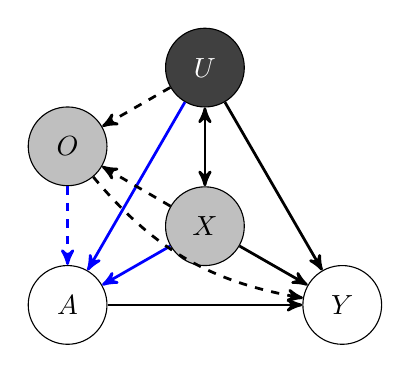
\begin{tikzpicture}
        \node[hiddenstate] (U) {$U$};
        \node[missingstate] (X) [below=of U] {$X$};
        \node[state] (A) [left=of X, xshift=.27cm, yshift=-1cm] {$A$};
        \node[state] (Y) [right=of X, xshift=-.27cm, yshift=-1cm] {$Y$};
        
        \path[double] (U) edge (X);
        \path[blue, normal] (U) edge (A);
        \path[blue, normal] (X) edge (A);
        \path[normal] (A) edge (Y);
        \path[normal] (U) edge (Y);
        \path[normal] (X) edge (Y);

        \node[missingstate] (O) [above=of A] {$O$};
        \path[blue, dashed, normal] (O) edge (A);
        \path[dashed, normal] (U) edge (O);
        \path[dashed, normal] (X) edge (O);
        \path[dashed, normal] (O) edge[bend left=-20] (Y);
    \end{tikzpicture}%
    \caption{DAG of the observational process in CCB} \label{fig:CCB_behavior}
  \end{subfigure}\qquad
\begin{subfigure}[b]{0.4\linewidth}
\centering
  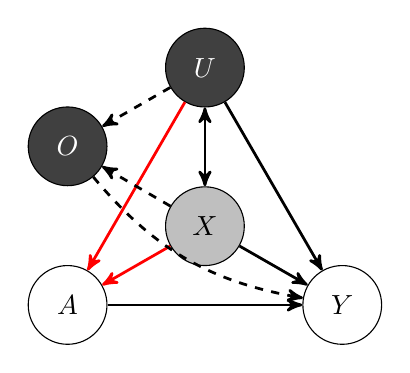
\begin{tikzpicture}  
      \node[hiddenstate] (U) {$U$};
        \node[missingstate] (X) [below=of U] {$X$};
        \node[state] (A) [left=of X, xshift=.27cm, yshift=-1cm] {$A$};
        \node[state] (Y) [right=of X, xshift=-.27cm, yshift=-1cm] {$Y$};
        
        \path[double] (U) edge (X);
        \path[red, normal] (U) edge (A);
        \path[red, normal] (X) edge (A);
        \path[normal] (A) edge (Y);
        \path[normal] (U) edge (Y);
        \path[normal] (X) edge (Y);

        \node[hiddenstate] (O) [above=of A] {$O$};
        \path[dashed, normal] (U) edge (O);
        \path[dashed, normal] (X) edge (O);
        \path[dashed, normal] (O) edge[bend left=-20] (Y);
\end{tikzpicture}
\caption{DAG of the interventional process in CCB} \label{fig:CCB_evaluation} 
\end{subfigure}
\caption{A DAG illustrating the observational and the interventional process in CCB. Here,  the white nodes represent the observed variables, the light gray nodes represent the variables missing not at random and the dark nodes represent unmeasured variables. A dashed line means the causal effect might either exist or not. }\label{fig:CCB}
\end{figure}  


\subsection{Observational Process}\label{sec:observational process}
The observational process describes how the offline dataset is collected, which is depicted in Figure \ref{fig:CCB_behavior}.
In the $t$-th trial of the observational process, the environment selects $(u_t, x_t, o_t)$ as a realization of $(U, X, O)$ according to the prior $\pr(u, x, o)$.
% {\color{orange} Maybe we could find a new name of $p$. Not sure if the reviewer will understand ``prior'' as the prior in Bayes.} 
The agent then conducts a treatment according to the observational policy $\pib: \cX\times \cO \times \cU\rightarrow \Delta(\cA)$. We remark that it is very common for the observational policy to be confounded by $U$, which can be understood as the agent's natural predilections, e.g., the playing agent in the observational procedure has a preference for certain treatments due to some hidden causes encoded by $U$ \citep{bareinboim2015bandits}.
After the treatment is conducted, a reward $Y$ depending on $(U, X, O, A)$ is received by the agent. The joint distribution $\pob$ in the observational process is thereby given by
\begin{align}\label{def:pob}
    \pob(u, x, o, a, y) = \pr(u, x, o) \cdot  \pib(a\given u, x, o) \cdot \pr(y\given u, x, o, a).
\end{align}
%Here, we provide two examples to illustrate the role of the side observations in the observational process.
Here we provide two typical examples of side observations in the observational process.
\begin{example}[Side observations as instrumental variable]\label{ex:IV}
In a confounded contextual bandit with instrumental variable (CCB-IV) shown in Figure \ref{fig:CCB-IV}, $O$ corresponds to instrumental variable $Z$, which is assumed to be independent of confounder $U$ and outcome $Y$. The observational policy is given by $\pib(a\given u, x, z)$.
\end{example}
\begin{example}[Side observations as proxy variables]\label{ex:PV}
In a confounded contextual bandit with proxy variables (CCB-PV) shown in Figure \ref{fig:CCB-PV}, $O$ corresponds to the negative controls $(Z, W)$. It is assumed that $W\indep A\given (U, X)$ holds for the outcome proxy $W$ and $Z\indep (Y, W)\given (A, X, U)$ holds for the treatment proxy $Z$. The observational policy is given by $\pib(a\given u, x, z)$.
\end{example}
Suppose there are $T$ trials in the observational process and the full dataset is denoted by $\tilde \cD = \{(u_t, x_t, a_t, y_t, o_t)\}_{t=1}^T$.
We emphasize that $\tilde\cD$ is not the dataset that will be used for policy learning due to the unmeasurement of the confounder $u_t$ and the missingness in both the contexts $x_t$ and the side observations $o_t$.
%The missingness mechanism is stated as follows.
We formally discuss the missingness mechanism in the following paragraph.

\paragraph{Missingness Mechanism. }
% We discuss the missingness issue in the observational process.
In addition to the unmeasurement of confounder $U$, we assume that side observations $O$ and context $X$ in our model are subject to missingness, which extends the missingness mechanism in \cite{yang2019causal, yang2017nonparametric}  %where they assume missingness to be not at random but  independent of outcome $Y$.
where missingness was assumed to be not at random but independent of outcome $Y$.
We denote the observed dataset as $\cD = \{(\check x_t, a_t, y_t, \check o_t)\}_{t=1}^T$, where $\check x_t$ and $\check o_t$ denote the context and the side observations that we truly observe.  
%For a rigorous illustration of the missingness, let random variables $R_X$ and $R_O$ denote the missingness indicators for $X$ and $O$, respectively.
Let random variables $R_X$ and $R_O$ denote the missingness indicators for $X$ and $O$, respectively.
Let $r_{X, t}$ and $r_{O, t}$ denote realizations of $R_X$ and $R_O$ in the $t$-th trial.
%Here, $r_{X, t}=1$ indicates that $x_t$ is not missing, i.e., $\check x_t=x_t$, and $r_{X, t}=0$ indicates that $x_t$ is missing, i.e., $\check x=\text{NaN}$ where NaN means missing value.
When $r_{X,t}=1$, the record of $x_t$ is not missing and $r_{X,t}=0$ indicates that the record of $x_t$ is lost.
We introduce a special dummy value $\text{None}$ to represent a missing record.
So $\check x_t$ takes values in $\{x_t, \text{None}\}$ by the rule of
\begin{equation*}
    \check x_t = \left\{
    \begin{aligned}
    & x_t & \quad \text{if } r_{X,t} = 1 \\
    & \text{None} & \quad \text{if } r_{X,t} = 0
    \end{aligned}
    \right.
\end{equation*}
%In contrast to assuming the observations to be missing randomly \citep{rubin2004multiple, qu2009propensity, crowe2010comparison, mitra2011estimating, seaman2014inverse}, we are considering a more challenging setting where the missingness is not at random, i.e., $R_X$ and $R_O$ are not independent of the model. 
In contrast to assuming the observations to be missing randomly \citep{rubin2004multiple, qu2009propensity, crowe2010comparison, mitra2011estimating, seaman2014inverse}, in this paper we study a more general and challenging setting in which the missingness is not at random, i.e., $R_X$ and $R_O$ are not independent of the model $(U,X,A,Y,O)$.
As $R_X$ and $R_O$ could be dependent of $(U,X,A,Y,O)$, our results covers the case of malicious adversarial missing.
We revisit the previous two examples to illustrate the missingness.
\begin{example}[Example \ref{ex:IV} revisited]
In the CCB-IV, we allow $R_X$ to be caused by $(Z, X, A)$ and $R_Z$ to be caused by $(Z, X)$.
\end{example}
\begin{example}[Example \ref{ex:PV} revisited]
In the CCB-PV, we allow $R_X$ to be caused by $X$, $R_Z$ to be caused by $(Z, U, A, X)$, and $R_W$ to be caused by $(W, X, A)$.
\end{example}
Identifying the causal effect in the presence of missingness is nontrivial because the missingness interferes with the structure of the observational dataset.
For instance, when conditioning on $R_X=1$ in the CCB-IV, the instrumental variable $Z$ might no longer be independent of the confounder $U$, which leads to failure of conventional identification approaches.
More details on the difficulties brought by the missingness mechanism as well as the method we use to address the missingness issue will be provided case by case in \S\ref{sec:Identification}. 



\subsection{Interventional Process} \label{sec:interventional process}
In the interventional process, an interventional policy is carried out after the model is learned from the offline dataset.
The interventional process is different from the observational process in the following three aspects: 
\begin{description}
\item[(i)] side observations $O$ appearing in the dataset are unmeasurable while context $X$ is fully measurable in the interventional process;
\item[(ii)] the agent follows an interventional policy $\pie:\cX\rightarrow \Delta(\cA)$ which is independent of $U$ and $O$ since they are unable to measure in the interventional process;
\item[(iii)] context $X$ follows a new marginal distribution $\tilde p(x)$ in the interventional process.
\end{description}
Aspect (i) indicates that only the context is revealed to the agent in the interventional process. Therefore, the interventional policy is context-dependent, as is stated in (ii).
We remark that (iii) can be understood through the idea of a marginal distribution shift in $X$ between the observational group and the interventional group, which is very common in real-world practice.
% Note that the unshifted context distribution can be viewed as a special case where $\tpr(x)=\pr(x)$. 
% We remark that it is common to have a shifted context distribution in practice. 
For example, when studying the effect of recommended ads' type ($A$) on the clicking rates ($Y$) with users' age ($X$) serving as the context, we might have an interventional group whose age distribution differs from the observational group.
Another example is the in-context learning paradigm,  where the task specification procedure can be viewed as "conditioning" the model on a certain context presented by the input texts/token \citep{brown2020language,radford2019language}.
Following (i)-(iii), the joint distribution $\pin{\pie}$ of random variables in the interventional process is given by
\begin{align}\label{def:pin}
    \pin{\pie}(u, x, o, a, y) = \tpr(x) \pr(u, o\given x) \pie(a\given x) \pr(y\given u, x, o, a).
\end{align}
Diagrammatic explanations of the interventional process are given in Figure \ref{fig:CCB_evaluation}. 
We see that the DAG of the interventional model is given by substituting the blue incoming edges to treatment $A$ encoded by $\pib$ in the observational model with the orange incoming edges encoded by $\pie$, while the remaining part of the DAG remains unchanged except for the marginal distribution of $X$.

\paragraph{Reward function and policy optimization.}
In the interventional process, the average reward $v^\pie$ is defined as
\begin{align}
    v^\pie = \EE_{\pin{\pie}}\sbr{Y},\label{def:v}
\end{align}
where $\EE_{\pin{\pie}}$ corresponds to the expectation taken with respect to $\pin{\pie}$ defined in \eqref{def:pin}.
Our target is to find  $\piestar\in\Pie:\cX\rightarrow \Delta(\cX)$ that optimizes the average reward, 
\begin{align*}
    \piestar= \arg\max_{\pie\in\Pie} v^\pie.
\end{align*}
Correspondingly, we define the performance metric as the following sub-optimality, 
\begin{align}
    \text{SubOpt}(\pie) = v^\piestar - v^\pie.\label{def: SubOpt}
\end{align}

In summary, our goal is to design a learning algorithm that returns a policy $\hat \pi$ based on the offline dataset $\cD$ collected in the observational process. Here the dataset is subject to unmeasured confounder and missingness. 

% For brevity, we denote by $g(x, a)$ the function to approximate the CATE and $\gstar(x, a)=\CATE(x, a)$ the actual CATE.

% where $v^\pie$ corresponds to the case $g(x,a)=\CATE(x, a)$.

\section{CAP Algorithm}\label{sec:CAP algorithm}
In this section, we first investigate the main challenges of such an offline bandit problem, including the issue of confounding and missing data and also the spurious correlation that arises in the decomposition of the sub-optimality in \S\ref{sec:challenges}.
We then put forward an algorithm framework named Causal-Adjusted Pessimistic (CAP) policy learning in the face of such challenges in \S\ref{sec:algorithm outline}.
\subsection{Challenges in the Offline Setting }\label{sec:challenges}
The offline learning problem in the CCB boils down to the following two questions:
(i) how to evaluate the average reward given an interventional policy; (ii) how to efficiently find an interventional policy that maximizes the average reward.
When trying to answer these two questions, we encounter two major challenges: (i) confounded and missing data; (ii) spurious correlation in the sub-optimality. 
We briefly discuss where these challenges stem from and what technologies we use to overcome these challenges in this subsection.
\paragraph{Challenges in average reward evaluation: confounded and missing data.}
The key to the problem of evaluating the average reward \eqref{def:v} in the interventional process is to learn the conditional average treatment effect (CATE) defined as
\begin{align*}
    \gstar(x, a)=\EEob\sbr{Y\given X=x, \doopt(A=a)}, 
\end{align*}
where $\EEob$ is an abbreviation for $\EE_{\pob}$.
Here, the do-calculus $\doopt(A=a)$ in the condition means that the expectation is taken with respect to the distribution obtained by deleting $\pib(a\given u, x, o)$ from the product decomposition of $\pob$ in \eqref{def:pob} and restricting $A=a$. 
% A diagrammatic explanation is given by removing all the blue arrows pointing into variable $A$ and then letting $A=a$ in Figure \ref{fig:CCB_behavior}. 
Learning the CATE is important since the average reward is related to the CATE by
\begin{align}\label{eq:v to CATE}
    v^\pie = \EE_{\pin{\pie}}\sbr{\gstar(X, A)}.
\end{align}
In the presence of confounding bias \citep{vanderweele2008causal, jager2008confounding}, learning the CATE needs tools borrowed from causal inference.
To control for the confounding bias, a typical way is to exploit side observations $O$ in the offline data \citep{lipsitch2010negative, singh2020kernel}.
Instances of controlling the confounding bias using side observations are presented in Examples \ref{ex:IV} and \ref{ex:PV} where instrumental variable (IV) \citep{cragg1993testing, arellano1995another,  newey2003instrumental} or proxy variables (PV) \citep{tchetgen2020introduction, ying2021proximal} are introduced for negative controls.

However, our problem is still challenging given the fact that the missingness bias is coupled with the confounding bias. 
Note that identification with outcome-independent missingness is rather trivial in the unconfounded contextual bandit setting with tuple $(X, A, Y, R_X)$ where $R_X$ is caused by $(X, A)$.
The simplest way is to use the dataset without missingness, i.e., conditioning on $R_X=1$ and estimate $\EEob\sbr{Y\given X=x, A=a, R_X=1}$. 
Such a method is valid since we have $R_X\indep Y\given (X, A)$ without confounders.
However, in the confounded contextual bandit setting, the causal effect is identified with the aid of side observations, and some model assumptions related to these side observations are broken when simply conditioning on $(R_X, R_O)=\ind$.
Take the CCB-IV case for instance. The IV independence assumption $Z\indep U\given X$ is broken by conditioning on $R_X=1$ since $R_X$ also depends on confounded action $A$. 
% Thereby, we have to find an alternative way to get around the missingness issue and identify the CATE. 
As we will show in \S\ref{sec:Identification}, the CATE learning problem is addressed by solving a novel integral equation system (IES), in which the integral equations are coupled together, and the CATE is obtained as the solution to the IES.

% We will formally state the missingness mechanism and show the methodologies to overcome such a problem in \S \ref{sec:Identification}. 

\paragraph{Challenges in policy optimization: spurious correlation.}
We discuss the second question on how to efficiently optimize the interventional policy.
Let $g$ denote an estimation of the CATE and $\gstar$ denote the exact $\CATE$ thereafter.
Following \eqref{eq:v to CATE}, we define the average reward function corresponding to $g$ and $\pie$ as
\begin{align}
    v(g, \pie) = \EE_{\pin{\pie}}\sbr{g(X, A)}.\label{def:v approx}
\end{align}
It is okay if we simply take a greedy policy $\hat \pi$ that maximizes $v(g, \pie)$. However, such a greedy policy can sometimes be misleading.
A little calculation of the sub-optimality helps gain intuition. 
We let $\tpr(x)=\ind(x=x_0)$ for brevity. By definition of the sub-optimality in \eqref{def: SubOpt} and the fact that $\hat \pie$ is greedy with respect to $g$, we have
\begin{align}
    \SubOpt(\hat \pi) \le \underbrace{\langle \gstar(x_0, \cdot)-g(x_0, \cdot), \piestar(\cdot\given x_0) \rangle}_{\text{(i)}} + \underbrace{\langle g(x_0,\cdot) - \gstar(x_0, \cdot), \hat\pie(\cdot\given x_0) \rangle}_{\text{(ii)}}. \label{eq:spurious subopt}
\end{align}
Note that $\piestar$ in term (i) is intrinsic to the bandit model and does not depend on $g$. In contrast, $\hat \pie$ in term (ii) is coupled with the estimated $g$, which yields the spurious correlation \citep{jin2021pessimism} and makes term (ii) hard to control.
Bounding term (ii) usually needs strong assumptions on the "uniform coverage" of the dataset $\cD$ as in the existing bandit and RL literature \citep{brandfonbrener2020bandit, tennenholtz2021bandits, laroche2019safe}, which occasionally fails to hold in practice. 


Instead, we adopt the technique of uncertainty quantification and pessimism to cope with the spurious correlation challenges. Similar techniques have been applied to other problems in the existing literature \citep{jin2021pessimism, uehara2021pessimistic, zhan2022offline, rashidinejad2021bridging}. Our work successfully integrates such techniques with the confounded and missing data scenarios. Specifically, we first construct a confidence set $\CICATE$ for the estimated $g$ based on the offline data such that $\gstar\in\CICATE$ holds with high probability.
If the policy is optimized with respect to $g\in\CICATE$ that minimizes $v(g, \cdot)$, it follows that $v(g, \hat \pie)\le v(\gstar, \hat \pie)$, and the spurious correlation in term (ii) vanishes. Then, the estimated policy is given by
\begin{align*}
    \piepessi = \arg\sup_{\pie\in\Pie} \inf_{g\in\CICATE} v(g, \pie).
\end{align*}
Moreover, it is also shown that pessimism can promote exploration \citep{auer2008near, azar2017minimax} and help weaken the assumptions on the concentrability coefficient or the data coverage \citep{buckman2020importance}.


\subsection{Algorithm Outline}\label{sec:algorithm outline}
% {\color{orange} Shall we put the subsection ``algorithm outline'' somewhere else? Section 2 is called ``problem formulation''.}
Now that we have answered the two questions raised in the last subsection by (i) identifying the CATE from an integral equation system (IES); (ii) optimizing the policy with a pessimistic estimator $g$ selected from some confidence set $\CICATE$.
What remains to clarify is how to construct the confidence set $\CICATE$ based on the IES.
As we will show in  \S\ref{sec:Estimation}, learning the CATE from the IES can be alternatively done by minimizing some empirical loss function $\cL_\cD(\vh)$ on the hypothesis class $\vH$, where $\vh$ is an estimated solution to the IES.
We are then inspired to construct the confidence set as a level set of $\vH$ with respect to metric $\cL_\cD(\cdot)$ and a threshold $e_\cD$. 
The whole procedure is summarized in the following Causal-Adjusted Pessimistic (CAP) policy learning algorithm.

\begin{algorithm}
\caption{Causal-Adjusted Pessimistic (CAP) policy learning}\label{alg:meta}
\small
\begin{algorithmic}
\REQUIRE dataset $\cD = \{\check x_t, a_t, y_t, \check o_t\}_{t=1}^T$ from the observational process, hypothesis space $\vH$, policy class $\Pie$, threshold $e_\cD$.
\STATE (i) Construct confidence set $\CICATE(e_\cD)$ as the level set of $\vH$ with respect to metric $\cL_\cD(\cdot)$ and threshold $e_\cD$.
\STATE (ii) $\piepessi=\arg\sup_{\pie\in\Pie}\inf_{g\in \CICATE(e_\cD)} v(g, \pie)$.
\ENSURE $\piepessi$.
\end{algorithmic}
\end{algorithm}
The IESs for identifying the CATE in both the CCB-IV and the CCB-PV settings are formulated in \S\ref{sec:Identification}, and a united form is presented with use of a linear operator $\cT$. 
Based on such a united form, the loss function $\cL_\cD(\cdot)$ and the confidence set $\CICATE$ is constructed using the technique of minimax estimator. More details about constructing $\CICATE$ are provided in \S\ref{sec:Estimation}. %The convergence results for the CAP algorithm in both the CCB-IV and the CCB-PV settings are provided in \S\ref{sec: theoretical results} together with an extension of the CCB-PV case in \S\ref{sec:extended CCB-PV}. Lastly, we apply the CAP algorithm under the CCB-IV setting to the linear Dynamic Treatment Regime (DTRs) problem in \S\ref{sec:DTR} and apply the CAP algorithm under the CCB-PV setting (with extended policy class) to the one-step linear Partially Observable Markov Decision Process (POMDP) in \S\ref{sec:POMDP}, both with the sub-optimality guaranteed to converge at a rate of $\tcO(T^{-1/2})$ theoretically.
 

\section{Background of Data-centric AI}
\label{sec:2}

This section provides a background of data-centric AI. Section~\ref{sec:2:1} defines the relevant concepts. Section~\ref{sec:2:2} discusses why data-centric AI is needed. Section~\ref{sec:2:3} draws a big picture of the related tasks and presents a goal-driven taxonomy to organize the existing literature. Section~\ref{sec:2:4} focuses on automation and human participation in data-centric AI.

\subsection{Definitions}
\label{sec:2:1}

Researchers have described data-centric AI in different ways. Ng et al. defined it as ``the discipline of systematically engineering the data used to build an AI system''~\cite{datacentricaihub}. Polyzotis and Zaharia described it as ``an exciting new research field that studies the problem of constructing high-quality datasets for machine learning''~\cite{polyzotis2021can}. Jarrahi et al. mentioned that data-centric AI ``advocates for a systematic and iterative approach to dealing with data issues''~\cite{jarrahi2022principles}. Miranda noted that data-centric AI focuses on the problems that ``do not only involve the type of model to use, but also the quality of data at hand''~\cite{miranda2021towards}. While all these descriptions have emphasized the importance of data, the scope of data-centric AI remains ambiguous, i.e., what tasks and techniques belong to data-centric AI. Such ambiguity could prevent us from grasping a concrete picture of this field. Before starting the survey, it is essential to define some relevant concepts:

\begin{itemize}
    \item \textbf{Artificial Intelligence (AI)}: AI is a broad and interdisciplinary field that tries to enable computers to have human intelligence to solve complex tasks~\cite{winston1984artificial}. A dominant technique for AI is machine learning, which leverages data to train predictive models to accomplish some tasks.
    \item \textbf{Data}: Data is a very general concept to describe a collection of values that convey information. In the context of AI, data is used to train machine learning models or serve as the model input to make predictions. Data can appear in various formats, such as tabular data, images, texts, audio, and video.
    \item \textbf{Training Data}: Training data is the data used in the training phase of machine learning models. The model leverages training data to adjust its parameters and make predictions.
    \item \textbf{Inference Data}: Inference data is the data used in the inference phase of machine learning models. On the one hand, it can evaluate the performance of the model after it has been trained. On the other hand, tuning the inference data can help obtain the desirable outputs, such as tuning prompts for language models~\cite{liu2023pre}.
    % It is used to measure the performance of the model after it has been trained. The evaluation data often does not overlap with the training data, so it can assess how well the model generalizes to unseen scenarios~\cite{reitermanova2010data}.
    \item \textbf{Data Maintenance}: Data maintenance refers to the process of maintaining the quality and reliability of data, which often involves efficient algorithms, tools, and infrastructures to understand and debug data. Data maintenance plays a crucial role in AI since it ensures training and inference data are accurate and consistent~\cite{jain2020overview}.
    \item \textbf{Data-centric AI}: Data-centric AI refers to a framework to develop, iterate, and maintain data for AI systems~\cite{zha2023data}. Data-centric AI involves the tasks and methods for building effective training data, designing proper inference data, and maintaining the data.
\end{itemize}


\subsection{Need for Data-centric AI} 
\label{sec:2:2}

In the past, AI was often viewed as a model-centric field, where the focus was on advancing model designs given fixed datasets.
%The research and development in the model-centric paradigm were largely driven by benchmark datasets, such as ImageNet~\cite{deng2009imagenet}, SQuAD~\cite{rajpurkar2016squad}, and Switchboard~\cite{bollacker2008freebase}.
%and Freebase~\cite{godfrey1992switchboard}.
However, the overwhelming reliance on fixed datasets does not necessarily lead to better model behavior in real-world applications, as it overlooks the breadth, difficulty, and fidelity of data to the underlying problem~\cite{mazumder2022dataperf}. Moreover, the models are often difficult to transfer from one problem to another since they are highly specialized and tailored to specific problems. Furthermore, undervaluing data quality could trigger data cascades~\cite{sambasivan2021everyone}, causing negative effects such as decreased accuracy and persistent biases~\cite{buolamwini2018gender}. This can severely hinder the applicability of AI systems, particularly in high-stakes domains.
 
Consequently, the attention of researchers and practitioners has gradually shifted toward data-centric AI to pursue data excellence~\cite{aroyo2022data}. 
% In contrast to model-centric AI, which merely focuses on iterating the model to improve performance using unchanged datasets,
Data-centric AI places a greater emphasis on enhancing the quality and quantity of the data with the model relatively more fixed. While this transition is still ongoing, we have already witnessed several accomplishments that shed light on its benefits. For example, the advancement of large language models is greatly dependent on the use of huge datasets~\cite{kenton2019bert,radford2018improving,radford2019language,brown2020language}. Compared to GPT-2~\cite{radford2019language}, GPT-3~\cite{brown2020language} only made minor modifications in the neural architecture while spending efforts collecting a significantly larger high-quality dataset for training. ChatGPT~\cite{ouyang2022training}, a remarkably successful application of GPT-3, adopts a similar neural architecture as GPT-3 and uses a reinforcement learning from human feedback procedure~\cite{christiano2017deep} to generate high-quality labeled data for fine-tuning. A new approach, known as prompt engineering~\cite{liu2023pre}, has seen significant success by focusing solely on tuning data inputs. The benefits of data-centric approaches can also be validated by practitioners~\cite{landingai,snorkelai,scaleai}. For instance, Landing AI, a computer vision company, observes improved accuracy, reduced development time, and more consistent and scalable methods from the adoption of data-centric approaches~\cite{landingai}. All these achievements demonstrate the promise of data-centric AI.

% Additionally, data-centric AI requires an in-depth understanding of the target problem domain and underlying data. Domain-specific data work, as an integral component in DCAI, is supplemented by model-centric techniques for the development of AI-based systems. Despite these essential differences between data-centric and model-centric AI,  the two paradigms are inherently complementary toward effective and efficient AI-based systems development.



% However, higher model performance on predefined and unchanged datasets does not necessarily means better model behavior. Moreover, the models are often difficult to transfer from one problem to another, as they are highly specialized and tailored to specific problems. 

%\dc{[Data-centric vs. Model-centric AI, extend the BlueSky track paper]}

%In previous years, model-centric AI (e.g., model structure design or advanced training strategy) has attracted much attention from academic research and industry.

%However, the maturity of model-centric AI leading to higher model performance in ``predefined" and unchanged test dataset does not necessarily results in better model behavior in practice.

%To overcome the susceptibility of data, the focus of researchers and practitioners gradually shifted toward data-centric AI emphasizing the role of data development and maintenance toward building effective and efficient AI-based systems.

% Data-centric AI differs from model-centric AI in terms of the main focus and data quality understanding. Specifically, data-centric AI generally holds the model fixed while optimizing data. Performance improvement is achieved by improving the quality and quantity of the data. Additionally, data-centric AI requires an in-depth understanding of the target problem domain and underlying data. Domain-specific data work, as an integral component in DCAI, is supplemented by model-centric techniques for the development of AI-based systems. Despite these essential differences between data-centric and model-centric AI,  the two paradigms are inherently complementary toward effective and efficient AI-based systems development.

% \dc{[Evidence showing that data-centric AI is the right direction. Citations]}

%Machine learning (ML) research facilitates massive progress in ML model architectures given a dataset that serves as benchmark to evaluate models. For example, large public datasets, such as ImageNet~\cite{deng2009imagenet}, SQuAD~\cite{rajpurkar2016squad}, Switchboard~\cite{bollacker2008freebase} and Freebase~\cite{godfrey1992switchboard}, compass ML research and facilitate model-centric AI developments. However, the overwhelming focus of benchmarking model performance in fixed large public datasets does not necessarily lead to better model behavior in real-world applications due to neglecting the breadth, difficulty, and fidelity of data to the underlying problem~\cite{mazumder2022dataperf}.

% With the plateaued development of model-centric AL development, data cascades problem in the real world has become evident and a key bottleneck for AI-based system development. Therefore, pursuing better data quality and data excellence ~\cite{aroyo2022data} are increasingly necessary and important. For example, as the model trained offline enter to wild, performance discrepancies, such as accuracy degradation and persistent bias issue~\cite{buolamwini2018gender,mehrabi2021survey,denton2020bringing}, usually appear in many applications. Such deployment discrepancy impedes the applicability of AI-based systems, such as health~\cite{wilkinson2020time} and data reuse~\cite{koch2021reduced}, where problems often resulting not from the model but the data that trained the models.

It is noteworthy that data-centric AI does not diminish the value of model-centric AI. Instead, these two paradigms are complementarily interwoven in building AI systems. On the one hand, model-centric methods can be used to achieve data-centric AI goals. For example, we can utilize a generation model, such as GAN~\cite{goodfellow2020generative,zhang2019self} and diffusion model~\cite{ho2020denoising,kingma2021variational,rombach2022high}, to perform data augmentation and generate more high-quality data. On the other hand, data-centric AI could facilitate the improvement of model-centric AI objectives. For instance, the increased availability of augmented data could inspire further advancements in model design. Therefore, in production scenarios, data and models tend to evolve alternatively in a constantly changing environment~\cite{polyzotis2021can}.



% \dc{[How to position data-centric AI?] Data-centric AI does not imply a negation of model-centric AI. Both are important. In practice, model-centric methods can be used to achieve data-centric AI goals. For example, we use GAN to do data augmentation, which uses a model for data-centric AI.}

%Domain-specific data work, as an integral component in DCAI, is supplemented by model-centric techniques for the development of AI-based systems. Despite these essential differences between data-centric and model-centric AI,  the two paradigms are inherently complementary toward effective and efficient AI-based systems development. The data-centric paradigm emerges from the ML community. The role of data-centric AI does not imply a negation of model-centric AI. Instead, data-centric and model-centric AI are indispensable and complementary to building effective AI-based systems. In practice, model-centric methods can be used to achieve data-centric AI goals. For example, we can adopt a generation model (e.g., GAN~\cite{goodfellow2020generative,zhang2019self} and diffusion model~\cite{ho2020denoising,kingma2021variational}) to conduct data augmentation. Therefore, more valuable samples are generated by model-centric AI for data-centric AI.  Similarly, data-centric AI can also facilitate the improvement of model-centric AI. For example, feature selection~\cite{li2017feature} and feature engineering~\cite{zheng2018feature,nargesian2017learning} are widely adopted to further advance model-centric AI performance in the industry. Many research discussions around data-centric or model-centric AI focus on how to generate high-quality data (e.g., diverse image collection~\cite{birnbaum2004human}, class definition, annotation strategy selection~\cite{wang2009multi,chong2009simultaneous}) or high-performance models (e.g, model structure design~\cite{he2016deep,ren2015faster}, loss function design~\cite{lin2017focal}) for specific ML problems once. However, for most production applications, data-centric and model-centric AI are usually alternatively evolved with each other. In other words, the datasets and models need to be updated alternatively and continuously. The key reason is that the environment that AI-based systems serve is inherently dynamic leading to dynamic gathered data. Additionally, the target problem definitions (e.g., identifying more diseases~\cite{stenton2020genetics}) can also change depending on customer demand or stakeholder stratagem.

\begin{figure}[t]
  \centering
    \includegraphics[width=0.85\textwidth]{figures/taxonomy.pdf}
  \caption{Data-centric AI framework.}
  \label{fig:taxonomy}
\end{figure}

\subsection{Tasks in Data-centric AI} 
\label{sec:2:3}



The ambitious movement to data-centric AI can not be achieved without making progress on concrete and specific tasks. Unfortunately, most of the existing literature has been focused on discussing the foundations and perspectives of data-centric AI without clearly specifying the associated tasks~\cite{polyzotis2021can,jarrahi2022principles,jakubik2022data,seedat2022dc}. As an effort to resolve this ambiguity, the recently proposed DataPerf benchmark~\cite{mazumder2022dataperf} has defined six data-centric AI tasks: training set creation, test set creation, selection algorithm, debugging algorithm, slicing algorithm, and valuation algorithm. However, this flat taxonomy can only partially cover the existing data-centric AI literature. For example, some crucial tasks such as data labeling~\cite{zhang2022survey} are not included. The selection algorithm only addresses instance selection but not feature selection~\cite{li2017feature}. The test set creation is restricted to selecting items from a supplemental set rather than generating a new set~\cite{saporta2002data}. Thus, a more nuanced taxonomy is necessary to fully encompass data-centric AI literature.

To gain a more comprehensive understanding of data-centric AI, we draw a big picture of the related tasks and present a goal-driven taxonomy to organize the existing literature in Figure~\ref{fig:taxonomy}. We divide data-centric AI into three goals: training data development, inference data development, and data maintenance, where each goal is associated with several sub-goals, and each task belongs to a sug-goal. We give a high-level overview of these goals below.




%Data-centric AI is a class of systematic techniques that develop, iterate, and maintain data for AI systems. ML community has continuously developed techniques to enhance data in many aspects. For example, active learning has been developed for decades to improve data label quality and efficiency~\cite{settles2009active}. Feature selection~\cite{li2017feature} aims to generate cleaner and more understandable data. Despite these individual initiatives for data, a comprehensive and systematic view of DCAI is still missing. In this paper, we provide a big picture of DCAI in Figure~\ref{fig:overview}, including training data development, evaluation data development, and data maintenance.

%The goal of DCAI is to establish up-to-date data benchmarks for model training and evaluation in the wild, which is beyond the role of training data construction. The reason behind the goal is two-fold. First, it is equally or even more crucial to build a trustful evaluation set for the purpose of model evaluation. Second, data is never created at once but rather in continuous maintenance in industrial applications. Therefore, it is essential to develop an infrastructure (e.g., efficient algorithms, and tools) to organize, store, understand, and debug data. We also provide a brief overview of these three key components, i.e., training data development, evaluation data development, and data maintenance, as follows.
\begin{itemize}
    \item \textbf{Training data development}: The goal of training data development is to collect and produce rich and high-quality training data to support the training of machine learning models. It consists of five sub-goals, including 1) data collection for gathering raw training data, 2) data labeling for adding informative labels, 3) data preparation for cleaning and transforming data, 4) data reduction for decreasing data size with potentially improved performance, and 5) data augmentation for enhancing data diversity without collecting more data.

    \item \textbf{Inference data development}: The objective is to create novel evaluation sets that can provide more granular insights into the model or trigger a specific capability of the model with engineered data inputs.
    %beyond relying solely on performance metrics (e.g., accuracy)
    There are three sub-goals in this effort: 1) in-distribution evaluation and 2) out-of-distribution evaluation aim to generate samples that adhere to or differ from the training data distribution, respectively, while 3) prompt enginerring tunes the prompt in language models to get the desired predictions. The tasks in inference data development are relatively open-ended since they are often designed to assess or unlock various capabilities of the model.
    % various aspects of the model, such as transferability, robustness, etc.
    
    % model-centric paradigm usually relies on some metrics (e.g., accuracy) calculated based on validation or test datasets. However, such evaluation sets do not necessarily reflect the actual model performance in the wild.  


    \item \textbf{Data maintenance}: In real-world applications, data is not created once but rather necessitates continuous maintenance. The purpose of data maintenance is to ensure the quality and reliability of data in a dynamic environment. It involves three essential sub-goals: 1) data understanding, which targets providing visualization and valuation of the complex data, enabling humans to gain valuable insights, 2) data quality assurance, which develops quantitative measurements and quality improvement strategies to monitor and repair data, and 3) data acceleration, which aims to devise efficient algorithms to supply the data in need via properly allocating resources and efficiently processing queries. Data maintenance plays a fundamental and supportive role in the data-centric AI framework, ensuring that the data in training and inference is accurate and reliable.
\end{itemize}

Following the three general goals, we survey various data-centric AI tasks, summarized in Table~\ref{tbl:tasksummary}.



\begin{table}[t]
\centering
\caption{Representative tasks under the data-centric AI framework.}
\footnotesize	
\label{tbl:tasksummary}
\setlength{\tabcolsep}{0.2pt}
\begin{tabular}{l|l|l} \toprule
\textbf{Goal} & \textbf{Sub-goal} & \textbf{Tasks} \\
\midrule

\multirow{6}{*}{\shortstack[l]{Training data\\ development}} & \cellcolor{gray!10}Collection & \cellcolor{gray!10}Dataset discovery~\cite{bogatu2020dataset}, data integration~\cite{stonebraker2018data}, raw data synthesis~\cite{lai2021revisiting}\\


~ & ~ & Crowdsourced labeling~\cite{kutlu2020annotator}, semi-supervised labeling~\cite{zoph2020rethinking}, active learning~\cite{ren2021survey}, \\

~ & \multirow{-2}{*}{Labeling} & data programming~\cite{ratner2016data}, distant supervision~\cite{mintz2009distant} \\

~ & \cellcolor{gray!10}Preparation & \cellcolor{gray!10}Data cleaning~\cite{zhang2016missing}, feature extraction~\cite{salau2019feature}, feature transformation~\cite{ali2014data}  \\

~ & Reduction & Feature selection~\cite{li2017feature}, dimensinality reduction~\cite{abdi2010principal}, instance selection~\cite{riquelme2003finding} \\

~ & \cellcolor{gray!10}Augmentation &  \cellcolor{gray!10}Basic manipulation~\cite{zhang2018mixup}, augmentation data synthesis~\cite{frid2018synthetic}, upsampling~\cite{zha2022towards}\\

\midrule

\multirow{3}{*}{\shortstack[l]{Inference data\\ development}} & In-distribution & Data slicing~\cite{chung2019slice}, algorithmic recourse~\cite{karimi2021algorithmic}\\
~ & \cellcolor{gray!10}Out-of-distribution & \cellcolor{gray!10}Generating adversarial samples~\cite{moosavi2016deepfool}, generating samples with distribution shift~\cite{koh2021wilds}\\
~ & Prompt engineering & Manual prompt engineering~\cite{schick2020few}, automated prompt engineering~\cite{wallace2019universal} \\

\midrule

\multirow{4}{*}{\shortstack[l]{Data\\ maintenance}} & \cellcolor{gray!10}~ & \cellcolor{gray!10}Visual summarization~\cite{burch2014benefits}, clustering for visualization~\cite{fahad2014survey}, \\
~ & \cellcolor{gray!10}\multirow{-2}{*}{Understanding} & \cellcolor{gray!10}visualization recommendation~\cite{wongsuphasawat2015voyager}, valuation~\cite{ghorbani2020distributional} \\
~ & Quality assurance & Quality assessment~\cite{sadiq2018data}, quality improvement~\cite{baylor2017tfx}\\
~ & \cellcolor{gray!10}Storage \& retrieval & \cellcolor{gray!10}Resource allocation~\cite{herodotou2011starfish}, query index selection~\cite{sun2019end}, query rewriting~\cite{baik2019bridging} \\

\bottomrule
\end{tabular}
\end{table}

\subsection{Automation and Human Participation in Data-centric AI} 

\label{sec:2:4}

% \dc{TODO: Add some discussion about why we need automation (because of the data size is too large)}

Data-centric AI consists of a spectrum of tasks related to different data lifecycle stages. To keep pace with the ever-growing size of the available data, in some data-centric AI tasks, it is imperative to develop automated algorithms to streamline the process. For example, there is an increasing interest in automation in data augmentation~\cite{cubuk2019autoaugment,zha2022towards}, and feature transformation~\cite{khurana2018feature}. Automation in these tasks will improve not only efficiency but also accuracy~\cite{mazumder2022dataperf}. Moreover, automation can facilitate the consistency of the results, reducing the chance of human errors. Whereas for some other tasks, human involvement is essential to ensure the data is consistent with our intentions. For example, humans often play an indispensable role in labeling data~\cite{zhang2022survey}, which helps machine learning algorithms learn to make the desired predictions. Whether human participation is needed depends on whether our objective is to align data with human expectations. In this survey, we categorize each paper into \emph{automation} and \emph{collaboration}, where the former focuses on automating the process, and the latter concerns human participation. Automation-oriented methods usually have different automation objectives. We can identify several levels of automation from the existing methods:

% In some tasks and the associated methods, human involvement is essential to ensure the data is consistent with our intentions. For example, humans play an indispensable role in labeling data~\cite{zhang2022survey}, which helps machine learning algorithms learn to make the desired predictions. Whereas for some other tasks, such as feature selection~\cite{li2017feature}, there is an increasing interest in automation to deal with a large amount of data more effectively and efficiently~\cite{liu2021automated}. Whether human participation is needed depends on whether our objective is to align data with human expectations, which is often determined by the nature of the tasks. In this survey, we categorize each task into \emph{automation} and \emph{collaboration} based on its objective, where the former focuses on automating the process, and the latter concerns human participation.



\begin{itemize}
    % \item \textbf{No automation:} Manually generating, processing, or debugging data based on domain knowledge from scratch.
    \item \textbf{Programmatic automation:} Using programs to deal with the data automatically. The programs are often designed based on some heuristics and statistical information.
    \item \textbf{Learning-based automation:} Learning automation strategies with optimization, e.g., minimizing an objective function. The methods at this level are often more flexible and adaptive but require additional costs for learning.
    %For example, AutoAugemnt or using GAN for data augmentation.
    \item \textbf{Pipeline automation:} Integrating and tuning a series of strategies across multiple tasks, which could help identify globally optimal strategies. However, tuning may incur significantly more costs.
\end{itemize}


% \dc{For some tasks, human participation is expected (e.g., ``labeling"), which leads to \emph{collaboration} between humans and machines. Some other tasks can be achieved without human involvement, which leads to \emph{automation}.}

% We defined different levels of collaboration as follows:

% \dc{Human participation depends on the nature of how the problem is formulated rather than methods that tackle the problems. For example, ``active XXX" or ``interactive XXX" often suggests that the problem must have human participation, no matter what methods we use.}

%We categorize the role of humans in a task as follows.


%\begin{itemize}
%    \item \textbf{No participation:} Humans do not participate in the task. The algorithms can accomplish tasks based on the data or resources without humans. For example, data augmentation.
%    \item \textbf{Partial participation:} Humans partially participate in the task. 
%    \item \textbf{Full participation:} Human involvement is required. Humans often need to supply information to achieve the goal. For example, data labeling and some tasks in data collection.
    
%\end{itemize}


% \dc{Automation is defined based on techniques but not problems. An active learning algorithm can also be very automated, even if it requires human involvement. For example, we can do meta-learning for active learning}

Note that this categorization does not intend to differentiate good and bad methods. For example, a pipeline automation method may not necessarily be better than programmatic automation solutions since it could be over-complicated in many scenarios. Instead, we aim to show insight into how automation has been applied to different data-centric goals and understand the literature from a global view. From another perspective, collaboration-oriented methods often require human participation in different forms. We can identify several degrees of human participation:



\begin{figure}[t]
  \centering
    \includegraphics[width=0.85\textwidth]{figures/survey_strategy.pdf}
  \caption{Data-centric AI papers are categorized into automation and collaboration depending on whether human participation is needed. Each method has a different level of automation or requires a different degree of human participation.}
  \label{fig:surveystrategy}
\end{figure}

\begin{itemize}
    % \item \textbf{Naive collaboration:} Manually generating, processing, or debugging data based on domain knowledge from scratch.
    \item \textbf{Full participation:} Humans fully control the process. The method assists humans in making decisions. The methods that require full participation can often align well with human intentions but can be costly.
    \item \textbf{Partial participation:} The method is in control of the process. However, humans need to intensively or continuously supply information, e.g., by providing a large amount of feedback or frequent interactions.
    \item \textbf{Minimum participation:} The method is in full control of the whole process and only consults humans when needed. Humans only participate when prompted or asked to do so. The methods that belong to this degree are often more desirable when encountering a massive amount of data and a limited budget for human efforts.
\end{itemize}

Similarly, the degree of human participation, to a certain extent, only reflects the tradeoff between efficiency (less human labor) and effectiveness (better aligned with humans). The selection of methods depends on the application domain and stakeholders' needs. To summarize, we design Figure~\ref{fig:surveystrategy} to organize the existing data-centric AI papers. We assign each paper to either a level of automation or a degree of human participation.
% In the following sections, we will review the existing methods and label them based on Figure~\ref{fig:surveystrategy}.


Some previous surveys only focus on specific scopes of data-centric AI, such as data augmentation~\cite{feng2021survey,wen2021time,shorten2019survey}, data labeling~\cite{zhang2022survey}, and feature selection~\cite{li2017feature}. The novelty of our paper is that it provides a holistic view of the tasks, methods, and benchmarks by providing a goal-driven taxonomy to organize the tasks followed by an automation- and collaboration-oriented design to categorize methods. Moreover, we discuss the needs, challenges, and future directions from the broad data-centric AI view, aiming to motivate collective initiatives to push forward this field.

% In the following sections, we will survey the literature under each data-centric AI goal following this structure.




 %\begin{itemize}
 %       \item \textbf{Indirect objectives:} Optimizing a proxy for learning. For example, we use GAN to learn to synthesize samples for data augmentation with GAN's objective, which forces the generated images to be similar to the original ones. However, this objective may not necessarily mean better augmentation performance.
 %       \item \textbf{Direct objectives:} Optimizing the true objective directly. For example, AutoAugment learns a policy to decide which augmentation strategies to use based on the validation performance. We could auto-tune the hyperparameters of GAN to maximize the performance metrics.
 %   \end{itemize}


%\subsection{Human Involvement in Data-centric ML (Remove)} 

%While many automated algorithms have been developed for data-centric ML, human involvement is essential in many scenarios, such as business understanding and data labeling.




%%%%%%%%%%%%%%%%%%%%%%%%%%%%%%%%%%%%%%%%%%%%%%%%%%%%%%%%%%%%%%%%%%%%%%%%%%%
%%%%%%%%%%%%%%%%%%%%%%%%%%%%%%%%%%%%%%%%%%%%%%%%%%%%%%%%%%%%%%%%%%%%%%%%%%%
%%% Inference rules for binary predicates
%%% Stephen J. Hegner
%%% Section 3
%%% 22 October 2018
%%%%%%%%%%%%%%%%%%%%%%%%%%%%%%%%%%%%%%%%%%%%%%%%%%%%%%%%%%%%%%%%%%%%%%%%%%%
%%%%%%%%%%%%%%%%%%%%%%%%%%%%%%%%%%%%%%%%%%%%%%%%%%%%%%%%%%%%%%%%%%%%%%%%%%%



 \section{Background on Proof Systems}\label{sec:proofsys}


   The results of this paper are based upon simple notions of
mathematical logic in general, and of propositional logic in
particular.  There are many excellent presentations of those subjects,
at various levels and from various perspectives, including, but not
limited to, \mycite{Monk76},
\mycite{Mendelson97_book}, \mycite{Enderton01_book},
\mycite{BenAri12_book}, and \mycite{Gallier15}.
  It is assumed that the reader is familiar with the basic ideas
presented in the appropriate chapters of those books.
   The purpose of this section is to establish notation and
terminology for proof systems.

 \begin{metalabpara}{notation}{}
     {Notation}\envlabel{not:not3}
    $\natnum$ denotes the set $\setbr{0,1,2,\ldots}$ of natural
numbers.
  Unless stated specifically to the contrary, an expression of the
form $\ccinterval{n_1}{n_2}$, with $n_1,n_2 \in \natnum$, denotes the
interval $\setdef{n \in \natnum}{n_1 \leq n \leq n_2}$.
    \par
  $\cardof{S}$ denotes the cardinality of the set $S$.
%    \par
%  For a sequence $p$, $\lengthof{p}$ denotes its length.
 \end{metalabpara}


 \begin{metalabpara}{context}{}
     {Context --- SMAS}\envlabel{ctxt:gransch}
   Unless stated specifically to the contrary, for the rest of this
paper, $\smasdef{G}$ will denote an arbitrary SMAS. 
 \end{metalabpara}


 \begin{metalabpara}{mydefinition}{}
     {WFFs for granule logic}\envlabel{def:granwff}
     At first glance, it might seem that $\allbinconstrgrsch{G}$ forms
a suitable set over which to express inference rules for binary
granule constraints.  However, that choice is too limiting.  For
example, to express that the subsumption relation $\gnleleq{}$ is
transitive, it would be necessary to have a separate rule of the form
   \[
    \tag{\ref{def:granwff}-1}
    \begin{prooftree}
       \hypoii{\subrulep{g_1}{g_2}}
              {\subrulep{g_2}{g_3}}
       \inferi{\subrulep{g_1}{g_3}}
    \end{prooftree}
   \]
 for each triple $\abr{g_1,g_2,g_3}$ of granules.  It would be far
better to be able to assert, with a single rule, that that such a
relationship holds for any triple of granules.  To this end, it is
appropriate to introduce a set
   $\setbr{\granvar{g}_1,\granvar{g}_2,\ldots,\granvar{g}_i,\ldots}$
 of granule variables, with the understanding that each such variable,
by default, may be bound to any granule.  The general transitivity
rule then becomes
   \[
    \tag{\ref{def:granwff}-2}
    \begin{prooftree}
       \hypoii{\subrulep{\granvar{g}_1}{\granvar{g}_2}}
              {\subrulep{\granvar{g}_2}{\granvar{g}_3}}
       \inferi{\subrulep{\granvar{g}_1}{\granvar{g}_3}}
    \end{prooftree}
   \]
 with $\abr{\granvar{g}_1,\granvar{g}_2,\granvar{g}_3}$
 representing any triple of granules, as already illustrated in
Fig.\ \ref{fig:infrulespmain}.
    In the case that variable may only be bound to certain granules,
an explicit qualifier may be used, as already illustrated in the rules
of Figs.\ \ref{fig:infrulespunsat} and \ref{fig:infrulesntaut} by
the use of  $|{\scriptscriptstyle(\granvar{g} \neq \bot)}$.
     \par
    To formalize this, begin by associating with $\granschemaname{G}$
a countable set
   $\varsetgrsch{G} =
 \preformat{\linebreak}
     \setbr{\granvar{g}_1,\granvar{g}_2,\ldots,\granvar{g}_i,\ldots}$
 of \emph{granule variables}, with
  $\varsetgrsch{G} \intersect \granulesofsch{G} = \emptyset$.
    Relative to this set, the \emph{positive binary well-formed
formulas} (or \emph{positive binary WFFs}) of $\granschemaname{G}$,
denoted $\pbinwffgrsch{G}$, is the set consisting of all expressions
of the forms $\subrulep{\gamma_1}{\gamma_2}$ and
$\disjrulep{\gamma_1}{\gamma_2}$ with
  $\gamma_1, \gamma_2 \in \granulesofsch{G} \union \varsetgrsch{G}$.
    In other words, $\pbinwffgrsch{G}$ is similar to
$\pbinconstrgrsch{G}$, except that both granule names and granule
variables may be used in the expressions.  Thus, in addition to the
members of $\pbinconstrgrsch{G}$, $\pbinwffgrsch{G}$ includes all
expressions of the forms
   $\subrulep{\granvar{g}_1}{g_2}$,
   $\subrulep{g_1}{\granvar{g}_2}$,
   $\subrulep{\granvar{g}_1}{\granvar{g}_2}$,
   $\disjrulep{\granvar{g}_1}{g_2}$,
   $\disjrulep{g_1}{\granvar{g}_2}$,
  and
   $\disjrulep{\granvar{g}_1}{\granvar{g}_2}$,
  for $\granvar{g}_1, \granvar{g}_2 \in \varsetgrsch{G}$
  and $g_1, g_2 \in \granulesofsch{G}$.
    Similarly, the \emph{negative binary WFFs} of $\granschemaname{G}$,
denoted $\nbinwffgrsch{G}$, is the set consisting of all expressions
of the forms $\nsubrulep{\gamma_1}{\gamma_2}$ and
$\ndisjrulep{\gamma_1}{\gamma_2}$ with
  $\gamma_1, \gamma_2 \in \granulesofsch{G} \union \varsetgrsch{G}$.
  Finally, the set of \emph{all binary WFFs} of $\granschemaname{G}$,
denoted $\allbinwffgrsch{G}$, is
  $\pbinwffgrsch{G} \union \nbinwffgrsch{G}$.
    \par
  A more formal and complete development of inference rules is found
in \envref{def:ruleproofnot} and that which follows.
 \end{metalabpara}


 \begin{metalabpara}{context}{}
     {Context --- Granule variables}\envlabel{ctxt:granvarset3}
   Unless stated specifically to the contrary, for the rest of this
paper,
   $\varsetgrsch{G} =
     \setbr{\granvar{g}_1,\granvar{g}_2,\ldots,\granvar{g}_i,\ldots}$
 will denote a countable set of granule variables for the SMAS
$\smasname{G}$ identified in \envref{ctxt:gransch}.
 \end{metalabpara}


 \begin{metalabpara}{mydefinition}{}
     {Semantics of WFFs}\envlabel{disc:semwff}
   To extend the notions of semantic entailment and model of
\envref{def:granstrsem} to WFFs involving variables, it is necessary
to bind those variables to granules.
 More precisely, define a \emph{substitution} for $\granschemaname{G}$
to be a possibly partial function
 $\fn{s}{\varsetgrsch{G}}{\varsetgrsch{G}\union\granulesofsch{G}}$.
  Define $\substgr{\varphi}{s}$ to be the WFF in which each variable
$\granvar{g}$ in the domain of $s$ is replaced by $s(\granvar{g})$.
  For example, if
   $s_0 = \setbr{\elfd{\granvar{g}_1}{g_3},
              \elfd{\granvar{g}_2}{g_4},
              \elfd{\granvar{g}_3}{\granvar{g}_3}}$,
  then
    $\substgr{\subrulep{\granvar{g}_1}{\granvar{g}_2}}{s_0}
        = \subrulep{g_3}{g_4}$.
  A \emph{ground} substitution $s$ is one for which
     $s(\varsetgrsch{G}) \subseteq \granulesofsch{G}$;
 in other words, for every $\granvar{g}$ for which s(\granvar{g}) is
defined, $s(\granvar{g})$ is a granule, never a variable.
   A substitution \emph{complete} for
 $\varphi \in \allbinwffgrsch{G}$
 if it is defined for every $\granvar{g} \in \varsetgrsch{G}$ which
occurs in $\varphi$.
  If $s$ is ground and complete for $\varphi$, say that $\varphi$
  \emph{holds for $s$} in a granule structure $\sigma$ 
 if $\substgr{\varphi}{s}$ holds in $\sigma$.
  Thus, a WFF is assigned a truth value once all of its variables have
been bound to granules.
   Now, for $\varphi_1, \varphi_2 \in \allbinwffgrsch{G}$,
  $\varphi_1 \sentails \varphi_2$, precisely in the case that
  $\substgr{\varphi_1}{s} \sentails \substgr{\varphi_2}{s}$ for every
ground substitution $s$ which is complete for both $\varphi_1$ and
$\varphi_2$.
   \par
  These ideas extend easily to $\Phi \subseteq \allbinwffgrsch{G}$.
  Define
   $\substgr{\Phi}{s}
      = \setdef{\substgr{\psi}{s}}{\psi \in \Phi}$,
 say that $s$ is \emph{complete} for $\Phi$ if it is complete for each
$\psi \in \Phi$, and for $\varphi \in \allbinwffgrsch{G}$, define
  $\Phi \sentails \varphi$ to hold iff
  $\substgr{\Phi}{s} \sentails \substgr{\varphi}{s}$ for every ground
substitution $s$ which is complete for both $\Phi$ and $\psi$,
  Similarly, for $\Phi' \subseteq \allbinwffgrsch{G}$,
    $\Phi \sentails \Phi'$ holds iff
  $\substgr{\Phi}{s} \sentails \substgr{\Phi'}{s}$ for every ground
substitution $s$ which is complete for $\Phi \union \Phi'$.
    \par
   Finally, satisfiability is always defined with respect to ground
substitutions.  More precisely,
 $\varphi \in \allbinwffgrsch{G}$
 (resp.\ $\Phi \subseteq \allbinwffgrsch{G}$)
 is \emph{satisfiable} if there is a ground substitution $s$ which is
complete for $\varphi$ (resp.\ for $\Phi$) with
n \mbox{$\modelsof{\substgr{\varphi}{s}} \neq \emptyset$}
 (resp.\
 \preformat{\linebreak}
 $\modelsof{\substgr{\Phi}{s}} \neq \emptyset$).
     \par
    It is easy to see that these notions for $\allbinwffgrsch{G}$
generalize those of \envref{def:granstrsem} for
$\allbinconstrgrsch{G}$.
 \end{metalabpara}

 \begin{metalabpara}{context}{}
     {General logical systems and negation}\envlabel{disc:logicsys}
    Many of the concepts introduced in the remainder of this section,
as well as in Secs.\ \ref{sec:negarm} and \ref{sec:ninfrules}, apply
in a more general setting than just $\allbinwffgrsch{G}$.  In this
spirit, the framework of a general logical system $\logicsys{L}$ will
be assumed as a context, as needed.  This context includes notions of
WFFs (denoted $\wffof{L}$), structure, model, and semantic entailment
(denoted $\sentails$).  It is assumed that $\logicsys{L}$ is
\emph{nontrivial} in that there is at least one
 $\varphi \in \wffof{L}$ which is satisfiable, and that it contains at
least one tautology $\true$ and one unsatisfiable assertion $\false$.
It is furthermore assumed that $\logicsys{L}$ has a negation operator,
with $\mlnot\varphi$ denoting the negation of $\varphi \in \wffof{L}$,
$\mlnot\mlnot\varphi$ equivalent to $\varphi$, and excluded middle
($\varphi$ and $\mlnot\varphi$ cannot both be satisfiable).  Further
detailed properties of $\logicsys{L}$ will not be developed here,
except as necessary in for a particular issue.  However, it is
worthwhile noting that there is no assumption that $\logicsys{L}$ be
closed under conjunction or disjunction.  In fact, the main example of
$\logicsys{L}$ in this paper, $\allbinwffgrsch{G}$, is closed under
neither.
     \par
     For readers not comfortable with this generalization, it suffices
to fix $\wffof{L}$ to be $\allbinwffgrsch{G}$ and $\sentails$ to be
the semantic entailment relation for that context.  The assertion
$\true$ (resp.\ $\false$) may be taken to be (a synonym for) any
element of $\pbintautgrsch{G}$ (resp.\ $\pbinunsatgrsch{G}$).
     In $\allbinwffgrsch{G}$, to avoid unnecessary pedantry,
$\nsubrulep{g_1}{g_2}$ (resp. $\ndisjrulep{g_1}{g_2}$), will be
regarded as the same WFF as $\mlnot\subrulep{g_1}{g_2}$
(resp. $\mlnot\disjrulep{g_1}{g_2}$).
%  Similarly, 
%$\subrulep{g_1}{g_2}$ (resp. $\disjrulep{g_1}{g_2}$), will be
%regarded as the same WFF as $\mlnot\nsubrulep{g_1}{g_2}$
%(resp. $\mlnot\ndisjrulep{g_1}{g_2}$).
   \end{metalabpara}


 \begin{metalabpara}{discussion}{}
     {Proof systems}\envlabel{disc:proofsys}
     Semantic entailment is a purely model-based means of relating
WFFs.  In order to deduce that a set of formulas implies
another; that is, to determine whether $\Phi \sentails \varphi$ holds,
a computational procedure is necessary.  This is the r{\^o}le of a
proof system.
     \par
     More precisely, a {proof system} $\proofsys{A}$ for a set
$\wffset{A} \subseteq \wffof{L}$ consists of a set of inference rules,
denoted
 $\infrulesof{A}$, by which new WFFs may be obtained from others. Let
$\Phi \subseteq \wffset{A}$ and let
 $\varphi \in \wffset{A}$.
  Write
 $\Phi \syntailss[\proofsys{A}] \varphi$ just in case
 $\varphi$ may be obtained from $\Phi$ by repeated application of the
inference rules of $\proofsys{A}$.
  Write
 $\Phi \syntailssi[\proofsys{A}] \varphi$ just in case
 $\varphi$ may be obtained from $\Phi$ by a single application of a
single inference rule of $\proofsys{A}$.
     \par
     The proof system $\proofsys{A}$ is \emph{sound} if whenever $\Phi
\syntailss[\proofsys{A}] \varphi$, then
 $\Phi \sentails \varphi$.  In words, only conclusions which are true
(in the sense of $\sentails$) may be proven.  Soundness is always an
essential property of a proof system.
     \par
     The proof system $\proofsys{A}$ is \emph{complete} if
whenever $\Phi \sentails \varphi$, then
 $\Phi \syntailss[\proofsys{A}] \varphi$.  In words, all inferences
which are true may be proven using $\proofsys{A}$.
 While not essential, completeness is nevertheless a highly desirable
property.
     \par
     The proof system $\proofsys{A}$ is \emph{decidable} if there is
an algorithm (which always terminates) for determining whether or not
$\Phi \syntailss[\proofsys{A}] \varphi$ holds.  All proof systems
considered in this report are decidable, since the set $\wffset{A}$
will always be finite.
 \end{metalabpara}


 \begin{metalabpara}{mydefinition}{}
       {Sat-conditional completeness}\envlabel{def:satcompl}
    A proof system $\proofsys{A}$ for $\wffset{A}$ is said to be
\emph{sat-complete} if for any satisfiable
  $\Phi \subseteq \wffset{A}$ and any $\varphi \in \wffset{A}$,
 $\Phi \sentails \varphi$ implies
  $\Phi \syntailss[\proofsys{A}] \varphi$.
   \par
    Thus, $\proofsys{A}$ is complete as long as the input set $\Phi$
is satisfiable, but it need not be complete in the case that $\Phi$ is
not satisfiable.
    (Of course, if $\Phi$ is not satisfiable, then
  $\Phi \sentails \varphi$ holds trivially, so sat-completeness is not
a serious limitation.  It does, require, however, that an alternate
means of detecting unsatisfiability be used.)
 \end{metalabpara}


 \begin{metalabpara}{mydefinition}{}
        {Notation for rules and proofs}\envlabel{def:ruleproofnot}
    The representation of proof rules employed in this paper is widely
used; the purpose here is to clarify terminology and notation.  A
generic rule is illustrated in (\ref{def:ruleproofnot}-1) below.
     \[
       \tag{\ref{def:ruleproofnot}-1}
       \begin{prooftree}
         \hypoi{\alpha_1~\alpha_2~\ldots~\alpha_k}
         \inferi[(r)]{\beta}
       \end{prooftree}
     \]
   The set $\setdef{\alpha_i}{i \in \ccinterval{1}{k}}
          \subseteq \wffof{L}$
consists of the \emph{antecedents} of the rule
 and is denoted $\antecedentsof{r}$.
   Similarly, $\beta \in \wffof{L}$ is the \emph{consequent},
 and is denoted $\consequentof{r}$.
    This rule denotes exactly that
  $\setdef{\alpha_i}{i \in \ccinterval{1}{k}}
                      \syntailss[\proofsys{A}] \beta$
  using a single application of the rule named $r$.
    If the rule name is clear from context, it may be omitted.
  If $k=0$; \ie, if
   $\setdef{\alpha_i}{i \in \ccinterval{1}{k}} = \emptyset$,
 then the rule expresses that $\beta$ is a tautology.  If $\beta$ is
$\false$, the rule expresses that
  $\alpha_1 \mland \alpha_2 \mland \ldots \mland \alpha_k$
 is unsatisfiable.
     \par
   As already suggested in \envref{def:granwff}, substitutions may be
applied to rules (as well as formulas).  For example,
(\ref{def:granwff}-1) is the result of applying the substitution
   $s_1 = \setbr{\elfd{\granvar{g}_1}{g_1},
              \elfd{\granvar{g}_2}{g_2},
              \elfd{\granvar{g}_3}{g_3}}$,
to (\ref{def:granwff}-2).
   If the set of substitutions is restricted, this is expressed via an
appropriate expression in angle brackets, as illustrated in
Figs. \ref{fig:infrulesptaut} and \ref{fig:infrulesntaut}.
     \par
   The result of applying a substitution to a rule is called an
\emph{instance} of that rule.  It will sometimes be useful to label a
rule instance in a proof.  For example, (\ref{def:ruleproofnot}-2) below
shows a single instance labelled with $d$.  In order to distinguish
rule names from labels, the former will always be written in
parentheses (as illustrated in (\ref{def:ruleproofnot}-1), while labels
will never be enclosed in parentheses.  Note that while a rule will in
general have only one name, there may be several instances of it (and
hence labels for those instances) in a single proof.
     \[
       \tag{\ref{def:ruleproofnot}-2}
       \begin{prooftree}
         \hypoi{\alpha_1~\alpha_2~\ldots~\alpha_k}
         \inferi[d]{\beta}
       \end{prooftree}
     \]
   As examples,
Figs.\ \ref{fig:infrulespmain}--\ref{fig:infrulesunsatpr} provide the
rules on granules which will be studied in this paper.  Later in the
paper, \envref{def:bininfpos}, \envref{def:swapclpbininf}, and
\envref{def:compprrules} provide the same rules, with names.
   \par
    A great advantage of the notation of \envref{def:ruleproofnot} is
that proofs involving the application of several rules may be
presented in a clear fashion visually.  For example, formulas
(\ref{def:ruleproofnot}-3) and (\ref{def:ruleproofnot}-4) below show
two ways of proving $\subrulep{g_1}{g_5}$ from the set
 \nlrightt
   $S_{\scriptsize\mbox{\ref{def:ruleproofnot}}}
      = \setbr{\subrulep{g_1}{g_2},
           \subrulep{g_2}{g_3},
           \subrulep{g_3}{g_4},
           \subrulep{g_4}{g_5}}$,
    \newline
 using the rule to the left in Fig.\ \ref{fig:infrulespmain}.
    The various deduction instances have been labelled, with
$d_1$--$d_3$ in (\ref{def:ruleproofnot}-3) and with $d_1'$--$d_3$ in
(\ref{def:ruleproofnot}-4).  All are instances of the rule
(\ref{def:granwff}-2).
 \begin{gather*}
    \tag{\ref{def:ruleproofnot}-3}
    \begin{prooftreem}
     \hypoii{\subrulep{g_1}{g_2}}
            {\subrulep{g_2}{g_3}}
     \inferi[d_1]{\subrulep{g_1}{g_3}}
     \hypoi{\subrulep{g_3}{g_4}}
     \inferii[d_2]{\subrulep{g_1}{g_4}}
     \hypoi{\subrulep{g_4}{g_5}}
     \inferii[d_3]{\subrulep{g_1}{g_5}}
    \end{prooftreem}
     \\[0.9em]
    \tag{\ref{def:ruleproofnot}-4}
    \begin{prooftreem}
     \hypoii{\subrulep{g_1}{g_2}}
            {\subrulep{g_2}{g_3}}
     \inferi[d_1']{\subrulep{g_1}{g_3}}
     \hypoii{\subrulep{g_3}{g_4}}
            {\subrulep{g_4}{g_5}}
     \inferi[d_2']{\subrulep{g_3}{g_5}}
     \inferii[d_3']{\subrulep{g_1}{g_5}}
    \end{prooftreem}
    \end{gather*}
    Diagrams such as (\ref{def:ruleproofnot}-3) and
(\ref{def:ruleproofnot}-3) are called \emph{proof trees} (for the
inference system under consideration).
     \par
    The \emph{antecedents} of a combined rule are the formulas which
are at the top level.  In both (\ref{def:ruleproofnot}-3) and
(\ref{def:ruleproofnot}-4), the set of
antecedents is $S_{\scriptsize\mbox{\ref{def:ruleproofnot}}}$.
    Each combined rule has a single \emph{consequent}, which is at the
bottom.  In both examples, it is $\subrulep{g_1}{g_5}$.
     \par
     A formula which occurs in a proof tree, other than as an
antecedent or consequent, is called an \emph{internal formula}.
     In (\ref{def:ruleproofnot}-3), the set
of internal formulas is
 $\setbr{\subrulep{g_1}{g_3}, \subrulep{g_1}{g_4}}$,
 while in (\ref{def:ruleproofnot}-4), it is
 $\setbr{\subrulep{g_1}{g_3}, \subrulep{g_3}{g_5}}$,
    \par
   Finally, a formula $\varphi$ which is regarded as an axiom will
always be regarded as a proof of itself.
 \end{metalabpara}


 \begin{metalabpara}{mydefinition}{}
        {Soundness and minimality of rules
                    and proof systems}\envlabel{def:minrule}
    Let $\proofsys{A}$ be a proof system for $\wffset{A}$, and let $r$
be a rule, as depicted in (\ref{def:minrule}-1) below.
     \[
       \tag{\ref{def:minrule}-1}
       \begin{prooftree}
         \hypoi{\alpha_1~\alpha_2~\ldots~\alpha_k}
         \inferi[(r)]{\beta}
       \end{prooftree}
     \]
  Call $r$ \emph{sound} if it produces consistent inference by
itself; \ie, if
     $\setbr{\alpha_1,\alpha_2,\ldots,\alpha_k} \sentails \beta$.
   \par
  Call a sound $r$ \emph{minimal} if whenever any $\alpha_i$ is
removed from the antecedents, the resulting rule $r'$, as shown in
(\ref{def:minrule}-2) below, is no longer sound.
     \[
       \tag{\ref{def:minrule}-2}
       \begin{prooftree}
         \hypoi{\alpha_1~\alpha_2~\ldots~\alpha_{i-1}~~
                     \alpha_{i+1}~\ldots~ \alpha_k}
         \inferi[(r')]{\beta}
       \end{prooftree}
     \]
  Put another way, the rule $r$ is minimal if for any
 $j \in \ccinterval{1}{k}$,
  $\setdef{\alpha_i}{i \in \ccinterval{1}{k}\setminus\setbr{i}}
    \not\sentails \beta$.
    \par
   Say that $\proofsys{A}$ is \emph{sound}
(resp.\ \emph{minimal}) if all members of $\infrulesof{A}$ have that
property.
 \end{metalabpara}


 \begin{metalabpara}{mydefinition}{}
        {Single-use vs.\ multiple-use proofs}\envlabel{def:single}
    It may be the case that an antecedent of a proof is used several
times.  For example, given the set
 \nlrightt
   $S_{\scriptsize\mbox{\ref{def:single}}}
      = \setbr{\subrulep{g_1}{g_2},
           \subrulep{g_2}{g_3},
           \subrulep{g_3}{g_2},
           \subrulep{g_2}{g_3},
           \subrulep{g_3}{g_4}}$,
 \newline
 of constraints, in the proof shown in
 (\ref{def:single}-1) below, each of $\subrulep{g_1}{g_2}$,
$\subrulep{g_1}{g_3}$, and $\subrulep{g_1}{g_3}$ is used more than once.
 \[
    \tag{\ref{def:single}-1}
    \begin{prooftreem}
     \hypoii{\subrulep{g_1}{g_2}}
            {\subrulep{g_2}{g_3}}
     \inferi[d_1]{\subrulep{g_1}{g_3}}
     \hypoi{\subrulep{g_3}{g_2}}
     \inferii[d_2]{\subrulep{g_1}{g_2}}
     \hypoi{\subrulep{g_2}{g_3}}
     \inferii[d_3]{\subrulep{g_1}{g_3}}
     \hypoi{\subrulep{g_3}{g_4}}
     \inferii[d_4]{\subrulep{g_1}{g_4}}
    \end{prooftreem}
 \]
  Call such a proof \emph{multiple use}.  On the other hand, call
proofs in which no formula occurs as an antecedent more than once
\emph{single use}.  The proofs of (\ref{def:ruleproofnot}-1) and
(\ref{def:ruleproofnot}-2) are single use.
     \par
   Call a proof system \emph{single use} if for any set
 $\setbr{\alpha_1,\alpha_2,\ldots,\alpha_k}$ of formulas, and any
single formula $\beta$, if there is a proof of $\beta$ from 
 $\setbr{\alpha_1,\alpha_2,\ldots,\alpha_k}$, then there is a
single-use proof.
     \par
   It is worth noting now that even though the proof of
(\ref{def:single}-1) is multiple use, a single-use proof is also
possible, as shown in (\ref{def:single}-2) below.
 \[
    \tag{\ref{def:single}-2}
    \begin{prooftreem}
     \hypoii{\subrulep{g_1}{g_2}}
            {\subrulep{g_2}{g_3}}
     \inferi[d_1]{\subrulep{g_1}{g_3}}
     \hypoi{\subrulep{g_3}{g_4}}
     \inferii[d_4]{\subrulep{g_1}{g_4}}
    \end{prooftreem}
 \]
  The proof systems developed in this paper for granule rules
are all single use, as will be established later.
     \par
   The idea of ``using up'' formulas, without permitting their re-use,
was introduced by Girard in the context of \emph{linear logic}
\mycite{Girard95_all}.
   Since it is not central to the results of this paper, linear logic
will not be considered further.
 \end{metalabpara}


 \begin{metalabpara}{summary}{}
         {Armstrong models}\envlabel{summ:armstrong}
      Let $\armctxt{C}$ be any set of sentences in a framework for
logic.  Given $\Phi \subseteq \cal{C}$, an \emph{Armstrong model} $M$
of $\Phi$, relative to $\armctxt{C}$, has the property that for every
 $\varphi \in \cal{C}$, it is the case that $M \in \modelsof{\varphi}$
iff $\Phi \sentails \varphi$.
    In other words, an Armstrong model $M$ is minimal in the sense that it
satisfies only those constraints of $\cal{C}$ which must be
satisfied in order for $M$ to be a model of $\Phi$.
     Say that $\cal{C}$ \emph{admits Armstrong models}, or that it is
an \emph{Armstrong context}, if every satisfiable subset of
$\armctxt{C}$ has such a model.
    See \mycite{Fagin82} for a comprehensive discussion of Armstrong
models, including a succinct characterization of the conditions under
which they exist \mycite[Thm.\ 3.1]{Fagin82}.
    \par
    In the context of this paper, the important case is
  $\cal{C} = \pbinconstrgrsch{G}$.  While it follows easily from the
more general result of \mycite[3.18]{HegnerRo17_inform} that
$\pbinconstrgrsch{G}$ admits Armstrong models, a much stronger result
is established in this section.  Specifically, it is shown how to
construct an Armstrong model, called the canonical model, for
$\pconstrgrsch{G}$.  Since $\granschemaname{G}$ is arbitrary, this is
essentially equivalent to showing how to construct a canonical model
for any
 $\Phi \subseteq \pbinconstrgrsch{G}$.  Using that model, it is shown
that the positive inference rules identified in Sec.\ \ref{sec:intro}
are both sound and complete.
 \end{metalabpara}



% !TEX root = paper.tex

\section{Theoretical Results} \label{sec: theoretical results}
Let $\vhstar$ denote the exact solution to \eqref{eq:united form}.
We allow the model to be misspecified, i.e., the exact solution might not be fully captured by the hypothesis space $\vH$.
To characterize the approximation error, we pose the following assumption on the realizability of the hypothesis class $\vH$.
\begin{assumption}[Realizability of hypothesis class]\label{asp:Realizability}
Let $\vareH>0$ be the minimal positive value such that there exists $\vhHstar=\{\hHstark{1}, \cdots, \hHstark{K-1}, \gHstar\}\in\vH$ satisfying,
\begin{itemize}
    \item[(i)] $\nbr{\vT\vhHstar}_{ \mu, 2} \le \vareH$, where $\nbr{\vT\vhHstar}_{\mu, 2}$  is the RMSE defined in \eqref{def:RMSE}.
    \item[(ii)] $\sup_{v\in\cV} \nbr{\gHstar-\gstar}_{v, 2}\le \vareH$, where $\cV=\{v: v(x, a)=\tpr(x)\pie(a\given x), \forall \pie\in\Pie\}$.
\end{itemize}
\end{assumption}
Here, (i) characterizes the approximation error of $\vhHstar$ under the metric $\nbr{\cT(\cdot)}_{\mu, 2}$ where $\mu$ represents the distribution in the dataset, and the approximation error in (ii) is the supremum over all the possible measure that is realizable by the policy class $\Pie$.
% The optimal estimator $\vhHstar=\{\hHstark{1}, \cdots, \hHstark{K}\}$ in the hypothesis class corresponding to the unconditional moment criteria \eqref{def:L} is defined as
% \begin{align}
%     \vhHstar=\arg\inf_{\vh\in\vH} \cL(\vh). \label{def:vhHstar}
% \end{align}
We remark that $\vhHstar$ can be softly viewed as the projection of $\vhstar$ onto the hypothesis space $\vH$ with approximation error $\vareH$.
We then pose the following assumption on the compatibility of the test function class $\Theta_k$.
\begin{assumption}[Compatibility of test function class]\label{asp:compatibility}
Suppose that for any $\vh\in\vH$ and for any $k\in\{1, \cdots, K\}$, it holds that
$\inf_{\theta_k\in\Theta_k} \nbr{\theta_k - \cT_k\vh}_{\mu_k, 2}\le \vareTheta$.
\end{assumption}
We give an example where the test function class has full compatibility. Following the discussion in \cite{dikkala2020minimax}, we consider a case where $\Theta_k$ lies in a Reproducing Kernel Hilbert space (RKHS) $\HH_{K_{\theta_k}}$ with RKHS kernel $K_{\theta_k}: \cZ_k\times\cZ_k\rightarrow \RR$. If $\alpha_k$ lies in another RKHS space $\HH_{K_{\alpha_k}}$ and the conditional density function $\pr(\vX, \vY_k\given \vZ_k)$ satisfies $\pr(\vX, \vY_k\given \cdot)\in \HH_{K_{\Theta_k}}$, we then have $\cT_k\vh\in \HH_{K_{\Theta_k}}$, which means that the dual function class has full compatibility. In addition, we pose the following assumption on the regularity of function classes $\vH$, $\vTheta$ and linear function $\alpha_k$.
\begin{assumption}[Regularity]\label{asp:regularity}
We assume that $\alpha_k$ is $L_{\alpha, 1}$-Lipschitz continuous with respect to $h_j$ and $Y_k$ for all  $j,k\in\{1, \cdots, K\}$.
We assume that the support of $Y_k$ is bounded, i.e., $\nbr{\text{supp}(Y_k)}_\infty\le L_Y$.
Moreover, we assume that $\sup_{h\in\vH}\norm{h}_\infty\le L_{h}$ and $\sup_{\theta\in\vTheta}\norm{\theta}_\infty\le L_{\theta}$.
\end{assumption}
We justify the regularity assumption by the examples of CCB-IV and CCB-PV.
Following Theorems \ref{thm:IV identification} and \ref{thm:PV ID}, 
we see that the continuity of $\alpha_k$ is apparent.
The regularity of $\vH$ and $\vTheta$ is easy to satisfy by choosing bounded function classes.
With bounded reward, it is straightforward that the linear function $\alpha_k(\vh, \vY_k)$ is globally bounded. Specifically, we can assume that  $\nbr{\alpha_k}_\infty\le L_\alpha$.

To characterize the properties of the confidence set Under these assumptions, we first define an event $\cE$ as
\begin{align}
    \cE &= \Big\{\abr{\EE_{\cD_k}\sbr{\alpha_k(\vh, \cY_k) \theta_k(\cZ_k)} - \EE_{\mu_k}\sbr{\alpha_k(\vh, \cY_k) \theta_k(\cZ_k)}} \le \eta_k\rbr{L_\alpha\nbr{\theta_k}_{\mu_k, 2}+\eta_k},\nend
    &\quad \abr{\norm{\theta_k}^2_{\cD_k, 2}-\norm{\theta_k}^2_{\mu_k, 2}}\le \frac 1 2\rbr{\norm{\theta_k}^2_{\mu_k, 2}+\eta_k^2}, 
    \forall \vh\in \vH, \forall \theta_k\in\Theta_k, \forall k\in\{1, \cdots, K\}\Big\}.\label{def:cE}
\end{align}
where $\eta_k$ bounds the maximal critic radius for function classes $\cQ_k$ and $\Theta_k$ with respect to $\xi\in(0, 1)$. Here, we define function class $\cQ_k$ as
\begin{align*}
    \cQ_k=\cbr{\alpha_k(\vh(\vX_k), \vY_k)\theta_k: \forall \vh\in\vH, \theta_k\in\Theta_k}.
\end{align*}
See \S\ref{app:critical radius} for calculation of the critical radius in the case of linear function class. 
We let $\eta^2=\sum_{k=1}^K \eta_k^2$ for simplicity. Now we give the following theorem, which shows that event $\cE$ holds with high probability and the confidence set built for uncertainty quantification enjoys some good properties.
\begin{theorem}[Uncertainty Quantification]\label{thm:Fast rate}
Suppose that Assumptions \ref{asp:Realizability}, \ref{asp:compatibility} and \ref{asp:regularity}  hold. 
Event $\cE$ holds with probability at least $1-2K\xi$ and the confidence set enjoys the following properties on $\cE$, 
\begin{itemize}
    \item[(i).] For the $\vhHstar$ satisfying Assumption \ref{asp:Realizability}, it holds that $\cL_\cD(\vhHstar) \le 2\vareH^2 + \rbr{2 L_\alpha^2+5 /4}\eta^2$. Moreover, if we set $e_\cD>2\vareH^2 + \rbr{2 L_\alpha^2+ 5/ 4}\eta^2$, it holds that $\gHstar\in\CICATE(e_\cD)$.
    \item[(ii).] For all $\vh\in\CIH(e_\cD)$, we have,
\begin{align*}
    \sup_{k\in\{1, \cdots, K\}}\nbr{\cT_k\vh}_{\mu_k, 2}\overset{\cE}{\lesssim} \cO(\vareTheta) + \cO(\vareH) + \cO\rbr{\sqrt{e_\cD}} +  \cO\rbr{\eta}.
\end{align*}
\end{itemize}
\begin{proof}
See \S\ref{pro:Fast rate} for a detailed proof.
\end{proof}
\end{theorem}
Theorem \ref{thm:Fast rate} shows that event $\cE$ holds with a high probability.
We see from (i) that it is theoretically guaranteed that $\vhHstar$ lies within the confidence set by properly setting the threshold $e_\cD$. As will be shown shortly after, such a property is vital for the use of pessimism.
Property (ii) in Theorem \ref{thm:Fast rate} shows that the RMSE for any $\vh\in\CIH(e_\cD)$ is well controlled on event $\cE$.
Now we are ready to present the convergence results for the sub-optimality defined in \eqref{def: SubOpt}. We give the following theorem on the sub-optimality for the CCB-IV.
\begin{theorem}[Convergence of sub-optimality for CCB-IV]\label{thm:IV subopt}
Suppose that Assumption 
\ref{asp:CCB-IV} for the CCB-IV model and the conditions in Remark \ref{rmk:IV existence} hold.
Suppose that Assumptions
\ref{asp:Realizability},  \ref{asp:compatibility}, and 
\ref{asp:regularity} for function classes $\vH$ and $\Theta$ hold.
The threshold $e_\cD$ for the confidence set is set to $e_{\cD}>2\vareH^2 + (2 L_\alpha^2+5/ 4)\eta^2$.
For the marginal distribution of context $\tpr$ in the interventional process and the optimal interventional policy $\piestar$, suppose that there exists $b_1:\cZ\rightarrow \RR$ satisfying 
\begin{align}
    \EEob\sbr{b_1(Z)\given A=a, X=x, R_Z=1} = \frac{\tpr(x)\piestar(a\given x)}{\pob(x, a\given R_Z=1)}.\label{cond:CCB-IV b1 exist}
\end{align}
The sub-optimality corresponding to $\piepessi$ for the CCB-IV is bounded on event $\cE$ with probability at least $1-4\xi$ by
\begin{align*}
    \SubOpt(\piepessi) \overset{\cE}{\lesssim} \sum_{k=1}^2 \nbr{b_k}_{\mu_k, 2}\cdot \big(\cO(\vareTheta) + \cO(\vareH) + \cO\rbr{\sqrt{e_\cD}} +  \cO\rbr{\eta}\big),
\end{align*}
where $b_2:\cA\times\cX\times\cZ\rightarrow \RR$ is defined as,
\begin{gather}
    b_2(a, x, z)=b_1(z)\frac{\pob(a, x, z\given R_Z=1)}{\pob(a, x, z\given(R_X, R_Z)=\ind)}.\label{eq:b2 IV}
\end{gather}
\begin{proof}
See \S\ref{proof: pessimism} and \S\ref{proof: subopt of IV} for a detailed proof.
\end{proof}
\end{theorem}
Similarly, the convergence of sub-optimality for CCB-PV is given by
\begin{theorem}[Convergence of sub-optimality for  CCB-PV]\label{thm:PV subopt}
    Suppose that Assumption 
\ref{asp:CCB-PV} for the CCB-PV model and the conditions in Remark \ref{rmk:PV existence} hold.
Suppose that Assumptions
\ref{asp:Realizability}, \ref{asp:compatibility}, and
\ref{asp:regularity} for function classes $\vH$ and $\Theta$ hold.
The threshold $e_\cD$ for the confidence set is set to $e_{\cD}>2\vareH^2 + (2 L_\alpha^2+5/ 4)\eta^2$.
For the marginal context distribution  $\tpr$ in the interventional process and the optimal interventional policy $\piestar$, suppose that there exists $b_1:\cX\times\cA\times\cZ\rightarrow\RR$ satisfying
    \begin{align}
        \EEob\sbr{b_1(X, A, Z)\given X=x, U=u, A=a, R_Z=\ind} = \frac{\pob(u\given x)\tpr(x)\piestar(a\given x)}{\pob(u, x, a\given  R_Z=1)}.\label{cond:CCB-PV b1 exist}
    \end{align}
    The sub-optimality corresponding to $\piepessi$ for the CCB-PV is bounded with probability at least $1-8\xi$ by
    \begin{align*}
        \SubOpt(\piepessi) \lesssim \sum_{k=1}^4 \nbr{b_k}_{\mu_k, 2}\cdot \big(\cO(\vareTheta) + \cO(\vareH) + \cO\rbr{\sqrt{e_\cD}} +  \cO\rbr{\eta}\big),
    \end{align*}
    where $b_2:\cA\times\cW\times\cX\times\cZ$, $b_3:\cW\times\cX\times\cA\times\cA'$ and $b_4:\cX\times\cA'\rightarrow\RR$ are defined as
    \begin{gather}
        b_2(a, w, x, z) = b_1(x, a, z)\frac{\pob(a, w, x\given (R_X, R_Z)=\ind)}{\pob(a, w, x\given (R_W, R_X, R_Z)=\ind)}.\nend
        b_3(w, x, a, a') = \frac{\tpr(x)\piestar(a'\given x)\pob(a, w\given x, R_X=1)}{u(a')\pob(x, a, w\given (R_W, R_X)=\ind)}, \quad
        b_4(x, a') = \frac{\tpr(x)\piestar(a'\given x)}{\pob(x\given R_X=1)u(a')}.\nonumber
    \end{gather}
\begin{proof}
See \S\ref{proof: pessimism} and \S\ref{proof: subopt of PV} for a detailed proof.
\end{proof}
\end{theorem}
\paragraph{Remarks on the existence of $b_1$.} We remark that the existence of $b_1$ in \eqref{cond:CCB-IV b1 exist} and \eqref{cond:CCB-PV b1 exist} are also related to the linear inverse problem,  as is discussed in \S\ref{app:linear inverse}. In the discrete setting, \eqref{cond:CCB-IV b1 exist} is automatically satisfied if the distribution shift ratio on the right-hand side is globally bounded. This is because we already have $\text{rank}(P(Z\given (A,X), R_Z=1))\ge |\cA|\times|\cX|$ by the IV completeness assumption and thus the Moore-Penrose inverse  $P(Z\given (A,X), R_Z=1)^+$ exists. Similarly, \eqref{cond:CCB-PV b1 exist} is also automatically satisfied in the discrete setting following the PV completeness assumption.

% \paragraph{Assumptions categories.} The assumptions that appear in Theorems \ref{thm:IV subopt} and \ref{thm:PV subopt} fall into the following three categories: 
% \begin{itemize}
%     \item[(i)] Assumptions on the causal model, which contains standard model assumptions on the IV/PV and the unconfounded and outcome-independent assumptions on the missingness indicators (Assumptions \ref{asp:CCB-IV} and \ref{asp:CCB-PV}). We also pose additional completeness conditions for the conditional moment equations to admit a solution (see arguments following Theorems \ref{thm:IV identification} and \ref{thm:PV ID}). Specifically, the completeness conditions on the outcome $Y$ with respect to the missing variables ensure that the information loss in the missing variable can be recovered for estimating the CATE.
%     \item[(ii)] Assumptions on the function classes for estimation, which contains the realizability assumption on the hypothesis class (Assumption \ref{asp:Realizability}), the compatibility assumption on the dual function class (Assumption \ref{asp:compatibility}), and the regularity assumption in Assumption \ref{asp:regularity}. Note that we don't require full realizability or compatibility.
%     \item[(iii)] Assumptions on distribution shift ratio, which contains the existence of $b_1$ to both \eqref{cond:CCB-IV b1 exist} and \eqref{cond:CCB-PV b1 exist} and bounded squared norm of functions $b_1, b_2, b_3$ and $b_4$. 
% \end{itemize}
% \paragraph{Distribution shift.} We remark that the following three factors contribute to the distribution shift arising in $b_k$: (i) the optimal interventional policy $\piestar$ differs from the observable policy $\pib$; (ii) the marginal distribution for the context $\tpr(x)$ in the interventional process differs from the marginal distribution for the context $\pob(x)$ in the dataset; (iii) the joint distribution with different conditions on the missing indicators differs since we have the issue of missing not at random.
% Notice that we only have to deal with the distribution shift corresponding to the optimal interventional policy $\piestar$ instead of the whole policy class $\Pie$, which makes the assumptions on bounded norm of the distribution shift ratio much weaker. 
% Such a benefit comes from the using of pessimism, which mitigates the error term (ii) with spurious correlation in \eqref{eq:spurious subopt} and only leaves the error in term (i) corresponding to the optimal interventional policy $\piestar$.
\paragraph{Significance of the main theorems.} 
Theorem \ref{thm:IV subopt} and \ref{thm:PV subopt} establish the convergence of the sub-optimality for the CAP algorithm in the offline confounded contextual bandit with missingness. 
Such results are achieved by using the minimax estimator, building a confidence set for the CATE, and integrating pessimism in the policy optimization step.
Our theories deal with model misspecification in the hypothesis space and the dual function class. Moreover, the sub-optimality does not rely on the “uniform coverage” of the observational dataset, e.g., uniformly lower bounded densities of visitation measures \citep{yang2020off, liao2020batch, duan2020minimax}.
This is because the distribution shift ratio $b_k$ only depends on the optimal policy $\piestar$, which is intrinsic to the bandit model, instead of the whole policy class $\Pie$. Therefore, we only require the dataset to “cover” certain distributions induced by $\piestar$.

\paragraph{Implications of the main theorems.} 
When it holds that $\eta\sim\tcO(n^{-1/2})$ (see \S\ref{app:critical radius} for a calculation of the critical radius of the linear function class) and $\vareH=\vareTheta=0$, by setting $e_\cD\sim\tcO(n^{-1})$, Theorem \ref{thm:IV subopt} and \ref{thm:PV subopt} indicates that $\SubOpt(\piepessi)\sim\tcO(n^{-1/2})$, which corresponds to a “fast statistical rate” for minimax estimation \citep{uehara2021finite}.
% Such a result relies on the analysis of the risk for the condidence set $\CIH(e_\cD)$ in Theorem \ref{thm:Fast rate}.
However, given the fact that the distribution shift ratio $b_k$ also stems from the missingness issue, we require some “compliance” of the data distribution with missingness in order for $b_k$ to be bounded. For instance, we require $\pob(a, x, z\given  R_Z=1)=\cO(\pob(a, x, z\given (R_X, R_Z)=\ind))$ for $b_2$ in \eqref{eq:b2 IV} to be bounded. Such a condition is reasonable if we consider a counterexample where $\pob(x_0\given R_Z)>0$ but $\pob(x_0\given (R_X, R_Z)=\ind)=0$ for $x_0\in \cX$, meaning that $x_0$ is totally missing from the observed dataset $\cD$. Therefore, there is no way to learn the CATE corresponding to $x_0$. 
On the other hand, following the discussion in \S\ref{app:critical radius} on the critical radius of a linear function class, we have $\eta_k\sim\cO(\sqrt{\log T_k/T_k})$ where $T_k=|\cD_k|$. Recall that $\cD_k$ may have different size since the conditional moment equations in the IES are subject to different missingness conditions. 
Therefore, we also require $T_k$ being of the same order of $T$ for $\SubOpt(\piepessi)$ to enjoy a fast statistical rate.

\vspace{-0.2cm}
\section{Numerical results}
\vspace{-0.15cm}
We now present experimental results of the proposed Algorithm \ref{alg_modular_sgd} on two exemplar problems in computed tomography (CT). 
The first set of experiments consider a simulated setting for quantitatively comparing the performance of Algorithm 
\ref{alg_modular_sgd} with the corresponding Hilbert and Banach space versions \eqref{eq:sgd_banach}.
%, in a setting where the ground truth data is known. Moreover, the impact of the stochastic setting is shown by comparing CPU times with the corresponding deterministic algorithms.   
In the second set of experiments we consider the dataset of real-world CT scans of a walnut \red{taken from} \url{doi:10.5281/zenodo.4279549}, with a fan beam geometry.
For these data, we utilise the insights from the first set of experiments and apply Algorithm \ref{alg_modular_sgd} in a setting with different noise modalities across the sinogram space.
%which allows investigating the use of variable exponents in the measurement space.
%
The experiments were conducted in \texttt{python}, using the open source  package \cite{CIL2021} for the tomographic backend.

\vspace{-0.25cm}

\paragraph{Hyper-parameter selection.} In the following experiments, we employ a decaying stepsize regime such that it satisfies the conditions of Theorem \ref{thm:as_lin_convergence} for the convergence of Banach space SGD, cf. \cite{Kereta2023}. A need for a decaying stepsize regime is common for stochastic gradient descent to mitigate the effects of inter-iterate variance.
Specifically, we use $\mu_k=\frac{\mu_{0}}{1+c(k/N_s)^\gamma}$, where $\mu_0>0$ is the initial stepsize, and $\gamma>0$ and $c>0$ control the decay speed. For the Hilbert space setting, $\mathbf{SGD}_2$, initial stepsize $\mu_0$ is given by the Lipschitz constant of the gradient of the objective function, namely $\mu_0=0.95/\max_{i}\|A_i\|^2$. For $\mathbf{SGD_p}$ and $\mathbf{SGD_{p_n,q_n}}$ the estimation of the respective H\"older continuity constant is more delicate and $\mu_0$ has to be tuned to guarantee convergence. However, its tuning is rather easy and the employ of a decaying strategy makes the choice of $\mu_0$ less critical.

As far as variable exponents are concerned, it is difficult (and somehow undesirable) to have a unified configuration as their selection is strictly problem-related. Parameters $(q_n)_n$ are related to the regularity of the measured sinograms as well as the different noise distributions considered.
For instance, when impulsive noise is considered, values of $q_-$ and $q_+$ closer to 1 are preferred while and for Gaussian noise values closer to $2$ are more effective. Solution space parameters $p_-$ and $p_+$ relate to the regularity of the solution to retrieve. As a consequence, their choice is intrinsically harder. We refer the reader to \cite{Bonino23}, where a comparison between different choices for $p_-$ and $p_+$ and different interpolation strategies is carried out for image deblurring with gradient descent \eqref{eq:gd_banach} in $\lpn$. 
%It is shown that the interpolation strategy used does not affect the reconstruction quality significantly, but the latter is more sensitive to the choice of a good interval $[p_-,p_+]$. However, the tuning of $p_-$, $p_+$, $q_-$, $q_+$ remains heuristic and specific to the particular problem and image considered. This will be object of further study.



\vspace{-0.25cm}
\paragraph{Simulated data.} We considered \eqref{eq:inv_prob} with $A$ given by the discrete Radon transform. For its definition we use a 2D parallel beam geometry, with 180 projection angles on a 1 angle separation, 256
detector elements, and pixel size of 0.1.
The synthetic phantom was provided by the CIL library, see Figure \ref{fig:phantom15}(b). 
After applying the forward operator, a high level (15\%) of salt-and-pepper noise is applied to the sinogram. The noisy sinogram is shown in Figure \ref{fig:phantom15}(a). 
\begin{figure}[t!]
\centering
\small
\setlength{\tabcolsep}{0pt}
\begin{tabular}{cccc}
% \includegraphics[height=0.22\textwidth]{Figures/Phantom15/sinogram.png}
{
\begin{tikzpicture}
\draw (0,0) node [anchor=south] {\includegraphics[height=0.22\textwidth]{{Figures/Phantom15/sinogram.png}}};%
% \spy on (0.1cm,-1.4cm) in node at (0.61cm, -.6cm);
\end{tikzpicture}
\hspace*{-4mm}
}
&
% \includegraphics[height=0.22\textwidth
\showpic{Figures/Phantom15/phantom15.png}\hspace*{-4mm} &
% \includegraphics[height=0.22\textwidth]
{
\begin{tikzpicture}[spy using outlines={rectangle, magnification=2, width = 0.75cm, height = 0.75cm,
connect spies, red, thick}]%
\draw (0,0) node [anchor=north] {\includegraphics[height=0.22\textwidth]{Figures/Phantom15/phantom15_rec_var_exp_40epochs.png}};%
\spy on (0.1cm,-1.4cm) in node at (0.61cm, -.6cm);
\end{tikzpicture}}
\hspace*{-4mm}
&
% \includegraphics[height=0.22\textwidth]
% \showpic
\begin{tikzpicture}[spy using outlines={rectangle, magnification=2, width = 0.75cm, height = 0.75cm,
connect spies, red, thick}]%
\draw (0,0) node [anchor=north] {\includegraphics[height=0.22\textwidth]{Figures/Phantom15/phantom15_px_stochastic.png} 
};%
\spy on (0.1cm,-1.4cm) in node at (0.54cm, -.61cm);
\end{tikzpicture}\hspace*{-4mm} \\
{\scriptsize{(a) Sinogram}} & {\scriptsize{(b) GT}} & {\scriptsize{(c) $\mathbf{SGD_{p_n,q_n}}$}} & {\scriptsize{(d) $(p_n)$ map}}
\end{tabular}
\caption{\footnotesize In (c) reconstruction of noisy sinogram (a) by $\mathbf{SGD_{p_n,q_n}}$, where $1.05= p_-\le(p_n)\le p_+=1.25$ is shown in (d) and $1.05=q_-\le(q_n)\le q_+=1.25$ is based on the model observation corresponding to $(p_n)$.}
\label{fig:phantom15}
\vspace{-0.25cm}
\end{figure}
\begin{figure}[t!]
\centering
\begin{subfigure}[b]{0.33\textwidth}
\includegraphics[height=3.5cm]{Figures/Phantom15/phantom15_mae.png}
\caption{MAE}
\label{fig:mae}
\end{subfigure}
\begin{subfigure}[b]{0.31\textwidth}
\includegraphics[height=3.5cm]{Figures/Phantom15/phantom15_psnr.png}
\caption{PSNR}
\label{fig:psnr}
\end{subfigure}
\begin{subfigure}[b]{0.32\textwidth}
\includegraphics[height=3.5cm]{Figures/Phantom15/phantom15_ssim.png}
\caption{SSIM}
\label{fig:ssim}
\end{subfigure}
\caption{\footnotesize Quality metrics along the first 100 epochs of $\mathbf{\text{SGD}_2}$; $\mathbf{\text{SGD}_{1.1}}$; $\mathbf{\text{SGD}_{p_n,q_n}}$ with and without adapting the exponent maps $(p_n)$. $\mathbf{\text{SGD}_2}$ is omitted from MAE and SSIM to improve the readability of the plots, due to its poor performance.}
\label{fig:phantom15_metrics}
\vspace{-0.15cm}
\end{figure}

\begin{table}[t]
\begin{center}
% \begin{tabular}{@{}cccc@{}}
% \centering
\begin{tabular}{c@{\hskip 0.2in}ccc@{\hskip 0.1in}cccccc}
% \toprule
\cmidrule[\heavyrulewidth]{2-10}
& \multicolumn{2}{c}{Deterministic} &      & \multicolumn{6}{c}{Stochastic ($\cdot=\mathbf{S}$)}                                            \\ \cmidrule{2-3} \cmidrule{5-10} 
Algorithm                   & It. & Tot. & & It.& Epoch & Tot.  & MAE & PSNR & SSIM \\ 
\cmidrule{1-3} \cmidrule{5-10} 
$\cdot\mathbf{GD_2}$                        & 0.44s         & 1324s & &0.02s         & 0.74s    & 74.4 s & 2.582{\rm e-}1   & 57.89  & 0.0304  \\
$\cdot\mathbf{GD_{1.1}}$                    & 0.43s         & 1297s & & 0.03s         & 0.81s    & 81.3s   & 3.671{\rm e-}3 & 82.64 & 0.9897   \\
$\cdot\mathbf{GD_{p_n,q_n}}$                     & 0.47s         & 1403s & & 0.03s         & 0.96s    & 96.5s  & 2.887{\rm e-}3 & 84.05 & 0.9927 \\
$\cdot\mathbf{GD_{p_n,q_n}}$ adapt.        & 0.44s         & 1317s & & 0.03s         & 0.91s    & 91.2s  &  1.777{\rm e-}3 & 88.10 & 0.9965  \\
Compute $(p_n),\ (q_n)$ & 0.45s         & 16s   & & 0.03s         & 0.8s      & 4.0s & - & - & -\\
\bottomrule
\end{tabular}
\end{center}
\caption{\footnotesize Comparison of per iteration cost and total CPU times after 3000 iterations for determistic algorithms and after 100 epochs for stochastic algorithm with $N_s=30$. MAE, PSNR and SSIM values for stochastic algorithms are computed after 40 epochs (before noise overfitting).
% \zeljko{maybe add some further details about how was this computed. Ie were metrics computed or not, what machine, averaging}
}
\label{tab:cputime}
\vspace{-0.7cm}
\end{table}
To compute subset data $A_i$ and $y_i$, the forward operator and the sinogram are pre-binned according to equally spaced views (w.r.t.~the number of subsets) of the scanner geometry. Subsequent subset data are offset from one another by the subset index $i$.
We consider $N_s=30$ batches. We compare results obtained by solving \eqref{eq:min_prob_general} by:
\begin{itemize}
    \item[] $\mathbf{{SGD}_{2}}$: $\mathcal{X}=\mathcal{Y}=\ell^2(\mathbb{R})$, $\mathcal{Y}=\ell^2(\mathbb{R})$, $f(x)=\frac{1}{2}\|Ax-y\|_2^2$ by SGD; 
    \item[] $\mathbf{{SGD}_p}$:  $\mathcal{X}=\mathcal{Y}=\ell^p(\mathbb{R})$, $p=1.1$, $f(x)=\frac{1}{p}\|Ax-y\|_p^p$ by Banach SGD  \eqref{eq:sgd_banach}; 
    \item[] $\mathbf{{SGD}_{p_n,q_n}}$: $\mathcal{X}=\lpn(\mathbb{R})$, $\mathcal{Y}=\ell^{(q_n)}(\R)$ for appropriately chosen exponent maps, $f(x)=\Bar{\rho}_{(q_n)}(Ax-y)$ with modular-based SGD Algorithm \ref{alg_modular_sgd}.
\end{itemize}
We considered step-sizes $\mu_k=\frac{\mu_{0}}{1+0.1(k/N_s)^\gamma}$, with $\mu_{0}$ and $\gamma$ which depend on the algorithm.\footnote{For $\mathbf{{SGD}_2}$ $\mu_0$ is set as $0.95/\max_{i}\|A_i\|^2$ and $\gamma=0.51$. For $\mathbf{{SGD}_p}$ and $\mathbf{{SGD}_{p_n,q_n}}$, we use $\mu_0=0.015$ with $\gamma=(p-1)/p+0.01$ and $\gamma=(p_--1)/p_-+0.01$ respectively.}
Spaces $\lpn(\mathbb{R})$ allow for variable exponent maps sensitive to local assumptions on both the solution and the measured data. 
A possible strategy for informed pixel-wise variable exponents consists in basing them on observed data (for $(q_n)$) and an approximation of the reconstruction (for $(p_n)$), as done in \cite{Bonino23,Lazzaretti_SISC22,Estatico2019}. 
To this end, we first compute an approximate reconstruction $\Tilde{x}\in\lpn(\mathbb{R})$ by running $\mathbf{{SGD}_p}$ in $\ell^{1.1}(\mathbb{R})$ for 5 epochs with a constant stepsize regime. 
The map $(p_n)$ is then computed via a linear interpolation of $\Tilde{x}$ between $p_{-}=1.05$ and $p_{+}=1.25$.  
The map $(q_n)$ is chosen as the linear interpolation between $q_{-}=1.05$ and $q_{+}=1.25$ of $A(p_n)$. 
The bounds $p_-,p_+$ and $q_-,q_+$ are chosen by prior assumptions on $y$ (sparse phantom) and on the noise observed (impulsive). 
% \red{ML: Should I show also the map $(p_n)$ in Figure \ref{fig:phantom15}?}
%
%The variable exponent setting also allows a further modification in the utilised solution space exponents.
%Provided that the iterates are improving the quality of the reconstruction, a sensible strategy would be to correspondingly update the solution space exponents $(p_n)$.
%To this end, we investigate
We also tested an adaptive strategy by updating $(p_n)$ based on the current solution estimate once every $\beta_\text{updates}$ epochs to adapt the exponents along the iterations. 
%We will refer to this strategy as adaptive modular-based SGD.

In Figure \ref{fig:phantom15_metrics}, we report the mean absolute error (MAE), peak signal to noise ratio (PSNR) and structural similarity index (SSIM) of the iterates $\xk$ w.r.t.~the known ground-truth phantom along the first 100 epochs. 
Since PSNR favours smoothness, it is thus beneficial for $\mathbf{{SGD}_2}$, whereas MAE promotes sparsity hence is beneficial for both $\mathbf{{SGD}_p}$ and $\mathbf{{SGD}_{p_n,q_n}}$.
Figure \ref{fig:psnr} shows that  Banach space algorithms provide better performance than $\mathbf{{SGD}_2}$ in all three quality metrics. 
Note that all the results show the well-known semi-convergence behaviour with respect to the metrics considered.
%: after the improvements throughout the first 40 epochs, the reconstructions start to overfit to data noise.
To avoid such behaviour an explicit regulariser or a sound early stopping criterion would be beneficial for reconstruction performance. 
We observe that the use variable exponents does not only improve all quality metrics, but also makes the algorithm more stable: the quality of the reconstructed solutions is significantly less sensitive to the number of epochs,  making possible early stopping strategies more robust. 

In Table \ref{tab:cputime}, the CPU times for deterministic ($\mathbf{GD_2}$, $\mathbf{GD_p}$ and $\mathbf{GD_{p_n,q_n}}$) approaches and stochastic ones ($\mathbf{SGD_2}$, $\mathbf{SGD_p}$ and $\mathbf{SGD_{p_n,q_n}}$) are compared.
%in terms of computational costs per iteration, epoch (for stochastic algorithms) and total time. 
%For the stochastic algorithms the MAE, PSNR and SSIM values after 40 epochs are reported.

\vspace{-0.2cm}
\paragraph{Real CT datasets: walnut.}
 We consider a cone beam CT dataset of a walnut \cite{Meaney2020}, from which we take a 2D fan beam sinograms from the centre plane of the cone. The cone beam data uses $0.5$ angle separation over the range $[0,360]$. The used sinogram is obtained by pre-binning the raw data by a factor of $8$, resulting in $280$ effective detector pixels.
The measurements have been post-processed for dark current and flat-field compensation.
As stepsize we used $\mu_k=\frac{\mu_{0}}{1+0.001(k/N_s)^\gamma}$, with $N_s=10$ subsets, and suitable $\mu_{0}$ and $\gamma$. \footnote{For $\mathbf{SGD}_2$ , $\mu_0=0.95/\max_{i}\|A_i\|^2$, $\gamma=0.51$. For $\mathbf{SGD}_{p_n,q_n}$ we $\mu_0=0.001$, $\gamma=0.58$.} 
Initial images are computed by $5$ epochs of $\mathbf{SGD_{1.4}}$  with a constant stepsize.
\begin{figure}[t!]
\centering
\small
\setlength{\tabcolsep}{0pt}
\begin{tabular}{cccc}
\begin{tikzpicture}[spy using outlines={rectangle, magnification=3, width = 0.75cm, height = 0.75cm,
connect spies, red, thick}]%
\draw (0,0) node [anchor=north] {\includegraphics[height=0.24\textwidth]{Figures/Walnut/Walnut_SNPSPeckle_Sinogram.pdf} 
};%
% \spy on (-0.4cm,-.65cm) in node at (0.75cm, -.55cm);
\end{tikzpicture}\hspace*{-3mm}
% \includegraphics[height=0.24\textwidth]{Figures/Walnut/Walnut_SNPSPeckle_Sinogram.pdf}
&
% \includegraphics[height=0.24\textwidth]
\begin{tikzpicture}[spy using outlines={rectangle, magnification=3, width = 0.75cm, height = 0.75cm,
connect spies, red, thick}]%
\draw (0,0) node [anchor=north] {\includegraphics[height=0.24\textwidth]{Figures/Walnut/Walnut_SNPSPeckle_Hilbert.pdf} 
};%
\spy on (-0.4cm,-.65cm) in node at (0.75cm, -.55cm);
\end{tikzpicture}\hspace*{-3mm}
% {Figures/Walnut/Walnut_SNPSPeckle_Hilbert.pdf} 
&
\begin{tikzpicture}[spy using outlines={rectangle, magnification=3, width = 0.75cm, height = 0.75cm,
connect spies, red, thick}]%
\draw (0,0) node [anchor=north] {\includegraphics[height=0.24\textwidth]{Figures/Walnut/Walnut_SNPSPeckle_NonAcq.pdf} 
};%
\spy on (-0.4cm,-.66cm) in node at (0.75cm, -.56cm);
\end{tikzpicture}\hspace*{-3mm} &
% \includegraphics[height=0.24\textwidth]{Figures/Walnut/Walnut_SNPSPeckle_NonAcq.pdf} &
% &\includegraphics[height=0.24\textwidth]
\begin{tikzpicture}[spy using outlines={rectangle, magnification=3, width = 0.75cm, height = 0.75cm,
connect spies, red, thick}]%
\draw (0,0) node [anchor=north] {\includegraphics[height=0.24\textwidth]{Figures/Walnut/Walnut_SNPSPeckle_Acq.pdf}  
};%
\spy on (-0.37cm,-.66cm) in node at (0.78cm, -.56cm);
\end{tikzpicture}\hspace*{-3mm}
% {Figures/Walnut/Walnut_SNPSPeckle_Acq.pdf} 
\\
{\scriptsize{(a) Sinogram}} & {\scriptsize{(b) SGD}} & {\scriptsize{(c) Constant exponents}} & {\scriptsize{(d) Variable exponents}}
\end{tabular}
\caption{\footnotesize{(a) Noisy sinogram with $10\%$ salt \& pepper (background) and speckle noise with $0$ mean and variance $0.01$ (foreground). (b) $\mathbf{SGD_2}$ result. (c) $\mathbf{SGD_{p_n,1.1}}$ result (d) $\mathbf{SGD_{p_n,q_n}}$ result. $p_-=1.2$, $p_+=1.3$, $q_{-}=1.1$ and $q_{+}=1.9$.}}
\label{fig:walnut_snpbackspecklefore_hilbert}
\vspace{-0.25cm}
\end{figure}
% We consider two reconstruction scenarios.

% \paragraph{Ablative study on impulse noise}
% A $0.10\%$ salt and pepper noise is applied to the sinogram, cf. Figure \ref{fig:walnut_snpnoise}(a).
% The walnut is then reconstructed using algorithm \ref{} \red{non-adaptive} with $p_Y=1.1$ in the acquisition space, and $p_{\max}=1.3,\,p_{\min}=1.1$ in the solution space. 
% The reconstructed image for $N_s=10$ is shown in Figure \ref{fig:walnut_snpnoise}(b). 
% In Figure \ref{fig:walnut_subset_study} we investigate the convergence of the objective value with respect to the number of subsets.
% The algorithms use the stepsize rule $\alpha_k=\frac{\alpha_{0,N_s}}{1+0.005(k/N_s)^\gamma}$, where $\gamma=2p_{\max}^\ast$, $N_s\in\{10,20,40\}$ is the number of used subsets, and $\alpha_{0,N_s}$ is chosen as large as possible to still ensure convergence. 

% \begin{figure}[h!]
% \centering
% \small
% \setlength{\tabcolsep}{0pt}
% \begin{tabular}{ccc}
% \includegraphics[width=0.19\textwidth]{Figures/Walnut/Walnut_Snp_high_sinogramVert.pdf} &
% % \includegraphics[width=0.4\textwidth]{Figures/Walnut/Walnut_Snp_high_hilbert.pdf}
% \includegraphics[width=0.38\textwidth]{Figures/Walnut/Walnut_Snp_high_Banach10.pdf}
% & \includegraphics[width=0.38\textwidth]{Figures/Walnut/Walnut_Snp_high_Banach10.pdf}
% % \includegraphics[width=0.38\textwidth]{Figures/Walnut/Walnut_Snp_high_Objective value.pdf}
% \\
% \scriptsize{(a) Sinogram} & \scriptsize{(b) Reconstruction with $N_s=10$} & {\scriptsize{(c) Objective value convergence}}
% \end{tabular}
% \caption{The sinogram in panel (a) contains $0.1$ salt and pepper noise. Panel (b) shows an exemplar reconstruction with $N_s=10$ subsets. In panel (c) we study the behaviour of the objective value with respect to the number of subsets. }
% \label{fig:walnut_snpnoise}
% \end{figure}
% % \red{maybe remove the hilbert and just have the sinogram, the banach recon and the objective value}


% \paragraph{Mixed sinogram noise}
% In the second set of experiments on the walnut we 
We consider a more delicate noise setting that requires exponential maps which vary in the acquisition domain.
Here, we assume that noise has a different effect on the background (zero entries) and the foreground (non-zero entries) of the clean sinogram.
Namely, we apply $10\%$ salt and pepper noise to the background, and speckle noise with mean $0$ and variance $0.01$ to the foreground, cf. Fig. \ref{fig:walnut_snpbackspecklefore_hilbert}(a) for the resulting noisy sinogram.
Notably, since this noise model has a non-uniform effect across the measurement data, Banach space methods favouring the adjustment of the Lebesgue exponents are expected to perform better than those making use of a constant value. 
Taking as a reference the result obtained by $\mathbf{SGD_2}$ (Fig. \ref{fig:walnut_snpbackspecklefore_hilbert}(b)), we compare here the effect of allowing variable exponents in the solution space only with the effect of allowing both maps $(p_n)$ and $(q_n)$ to be chosen.
By choosing $(p_n)$ based on the initial image and interpolating it between $p_{-}=1.2$ and $p_{+}=1.3$ we then compare $\mathbf{SGD_{p_n,1.1}}$ (i.e., fixed exponent $q=1.1$ in the measurement space), cf.~ Fig. \ref{fig:walnut_snpbackspecklefore_hilbert}(c), with $\mathbf{SGD_{p_n,q_n}}$ where $(p_n)$ is as before while $(q_n)$ is chosen from the sinogram by interpolating between $q_{-}=1.1$ and $q_{+}=1.9$, cf.~Fig. \ref{fig:walnut_snpbackspecklefore_hilbert}(d).
The results show that a flexible framework where both maps $(p_n)$ and $(q_n)$ adapt to local contents are more suited for dealing with this challenging scenario.




% !TEX root = paper.tex
%\begin{flushleft}
\section{Application of CCB-IV: Linear Dynamic Treatment Regimes} \label{sec:DTR}




% \begin{figure}
% \centering
%   % Requires \usepackage{graphicx}
%   \subfloat[DAG of the observational process in DTR]{\includegraphics[width=4.5cm]{figure/DTR_behavior.pdf}
%   % \label{fig:DTR behavior}
%   }
%   \hspace{1.5cm}
%   \subfloat[DAG of the interventional process in DTR]{\includegraphics[width=4.5cm]{figure/DTR_evaluation.pdf}
%   % \label{fig:DTR evaluation}
%   }\\
% %   \vspace{0.5cm}
%    \caption{A DAG illustrating the DTR model. Note that $Y_2$ depends on the whole trajectory $H$}\label{fig:DTR}
% \end{figure}
\paragraph{Background.} Dynamic treatment regimes (DTRs) is an extension of the individualized treatment rules (ITRs) to multi-steps. Estimating optimal policy can be challenging with unmeasured confounders in the observational dataset
\cite{chen2021estimating, qi2021proximal, NEURIPS2019_8252831b, singh2022automatic}.
We consider a DTRs with two steps, which is graphically represented in Figure \ref{fig:DTR}. 

\begin{figure}[h]  
\centering 
  \begin{subfigure}[b]{0.4\linewidth}
  \centering
    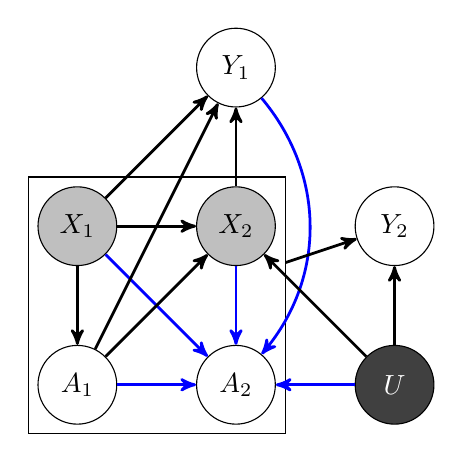
\begin{tikzpicture}
        \node[missingstate] (X1) {$X_1$};
        \node[missingstate] (X2) [right=of X1] {$X_2$};
        \node[state] (A1) [below=of X1] {$A_1$};
        \node[state] (A2) [below=of X2] {$A_2$};
        \node[state] (Y1) [above=of X2] {$Y_1$};
        \node[state] (Y2) [right=of X2] {$Y_2$};
        \node[hiddenstate] (U) [below=of Y2] {$U$};
        \node[draw, fit=(X1) (X2) (A1) (A2)] (H) {};

        \path[normal] (X1) edge (A1);
        \path[normal, blue] (X1) edge (A2);
        \path[normal] (X1) edge (X2);
        \path[normal] (X1) edge (Y1);
        \path[normal, blue] (X2) edge (A2);
        \path[normal] (X2) edge (Y1);
        \path[normal] (A1) edge (Y1);
        \path[normal] (A1) edge (X2);
        \path[normal, blue] (A1) edge (A2);
        \path[normal, blue] (Y1) edge[bend left=40] (A2);
        \path[normal] (U) edge (X2);
        \path[normal] (U) edge (Y2);
        \path[normal, blue] (U) edge (A2);
        \path[normal] (H) edge (Y2);
    \end{tikzpicture}
    \caption{DAG of the observational process in DTR}
  \end{subfigure}\qquad
\begin{subfigure}[b]{0.4\linewidth}
\centering
  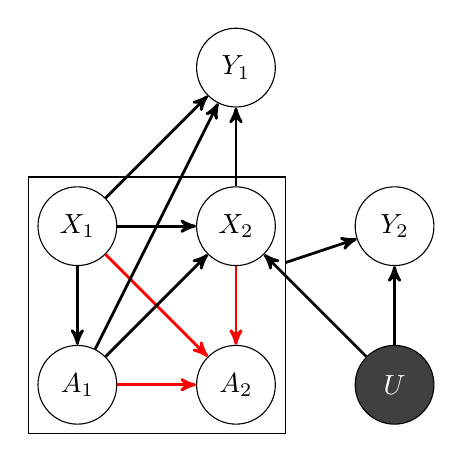
\begin{tikzpicture}  
        \node[state] (X1) {$X_1$};
        \node[state] (X2) [right=of X1] {$X_2$};
        \node[state] (A1) [below=of X1] {$A_1$};
        \node[state] (A2) [below=of X2] {$A_2$};
        \node[state] (Y1) [above=of X2] {$Y_1$};
        \node[state] (Y2) [right=of X2] {$Y_2$};
        \node[hiddenstate] (U) [below=of Y2] {$U$};
        \node[draw, fit=(X1) (X2) (A1) (A2)] (H) {};

        \path[normal] (X1) edge (A1);
        \path[normal, red] (X1) edge (A2);
        \path[normal] (X1) edge (X2);
        \path[normal] (X1) edge (Y1);
        \path[normal, red] (X2) edge (A2);
        \path[normal] (X2) edge (Y1);
        \path[normal] (A1) edge (Y1);
        \path[normal] (A1) edge (X2);
        \path[normal, red] (A1) edge (A2);
        \path[normal] (U) edge (X2);
        \path[normal] (U) edge (Y2);
        \path[normal] (H) edge (Y2);
\end{tikzpicture}
\caption{DAG of the interventional process in DTR}
\end{subfigure}
\caption{A DAG illustrating the DTR model. Note that $Y_2$ depends on the whole trajectory $H$}\label{fig:DTR}
\end{figure}  

In the observational process, at stage $i\in\{1, 2\}$, the treatment $A_i$ is selected based on the current state $X_i$ and the historical information $\{(X_j, A_j, Y_j)\}_{j=1}^{i-1}$. Then the state transits to $X_{i+1}$ and a reward $Y_i$ is generated. At the second state, $X_2$, $A_2$ and $Y_2$ are confounded by an unmeasured confounder $U$. Since the first step is not influenced by $U$, we have $Y_1\indep U\given (X_1, X_2, A_1)$. Therefore, we see that the first state reward $Y_1$ serves as an instrumental variable to $A_2$. Here, we provide table \ref{tab:DTRs} to illustrate the mapping from this two-stage DTRs to the CCB-IV model. 
\begin{table}[]
    \centering
    \begin{tabular}{  c  c c c} 
  \hline
  Variable Type & Two-step DTRs & Observability in $\cD$ & Correspondence to CCB-IV\\ 
  \hline
  confounder    &   $U$                 & unobservable  &   $U$\\
  context       &   $(X_1, X_2, A_1)$   & partially missing  & $X$ \\
  treatment     &   $A_2$               & observable & $A$\\
  outcome       &   $Y_2$               & observable & $Y$\\
  IV            &   $Y_1$               & observable & $Z$\\
  \hline
\end{tabular}
    \caption{Mapping of variables from the two-state DTRs to the CCB-IV.}
    \label{tab:DTRs}
\end{table}
We assume that $Y_2=f(X_1, X_2, A_1, A_2)+\varepsilon$ where $\varepsilon\indep (A_1, A_2)\given (U, X_1, X_2)$ and that $Y_1$ and $Y_2$ are fully observed, which satisfies the structured reward assumption. 
For $Y_1$ to function as an IV, we require that $Y_1$ is complete over $(X_1, X_2, A_1, A_2)$. 
Additionally, in the observational process, the missingness indicator $R_{X_1}$ is caused by $(X_1, A_1)$ and the missingness indicator $R_{X_2}$ is caused by $(X_1, A_1, X_2, A_2)$. 
Therefore, the model assumptions for CCB-IV are satisfied. 
By Theorem \ref{thm:IV identification}, the CATE $g(x_1, a_1, x_2, a_2)=\EEob\sbr{Y_2\given x_1, a_1, x_2, \doopt(a_2)}$ is identified by
%\begin{gather}
\begin{align}
    &\EEob\sbr{h_1(A, Y) - Y_2\given Y_1=y_1}=0, \label{eq:DTR ID 1}\\
    &\EEob\sbr{g(X, A)-h_1(A, Y) \given (X, A, Y_1)=(x, a, y_1), (R_{X_1}, R_{X_2})=\ind}=0.\label{eq:DTR ID 2}
\end{align}
%\end{gather}
We assume that the solutions $h_1$ and $g$ always exist, which requires certain completeness conditions for $Y_2$ to restore the missingness in $X_1$ and $X_2$.
Here, we let $X=(X_1, X_2)$, $A=(A_1, A_2)$ and $Y=(Y_1, Y_2)$ in the remaining part of the section for DTRs example. 
% Notice that the definitions of $X$, $A$ and $Y$ here are different from their previous ones. 
Note that $Y_2\indep \pib_1\given (X_1, A_1, X_2)$ in the observational settings, since $A_1$ is not confounded. We thereby have $g(x, a)=\EEob\sbr{Y_2\given x, \doopt(a)}$.
Our optimization target thereby corresponds to maximizing the average reward function on $\pie=(\pi_1, \pi_2)\in\Pi$,
\begin{align*}
    v(g, \pie)=&\int_{\cX\times\cA} g(x,a) \tpr(x_1) \pob(x_2\given x_1, a_1)   \pi_1(a_1\given x_1) \pi_2(a_2\given x_1, a_1, x_2)
    \rd x\rd a,
\end{align*}
where we assume that $\pob(x_2\given x_1, a_1)$ is already known for brevity, although a little extension of our framework is capable of dealing with unknown $\pob(x_2\given x_1, a_1)$ by learning from data. Moreover, we only consider $Y_2$ as the reward. We remark that, since the first stage is not confounded, $\EEob\sbr{Y_1\given x_1, \doopt(a_1), x_2}$ can also be easily learned and integrated into the average reward. Now we pose the following assumptions on the linearity of the DTRs model.

\paragraph{Linear function class.} We make the following assumptions to ensure the existence of the bridge functions and the linearity of our DTRs model.
\begin{assumption}[Existence of linear bridge functions]\label{asp:DTRs linear 1}
We assume that a solution $\vhstar=(\hstark{1}, \gstar)$ exists to the IES given by \eqref{eq:DTR ID 1} and \eqref{eq:DTR ID 2}. Furthermore, we assume that $\hstark{1}, \gstar$ fall into the following function classes,
%\begin{gather*}
\begin{align*}
    &\cH_1=\{h_1\given h_1(\cdot)=w_1^\top \phi_1(\cdot), \nbr{w_1}_2\le C_1, \nbr{\phi_1(\cdot)}_2\le 1\}, \\
    &\cG=\{g\given g(\cdot)=w_2^\top \phi_2(\cdot), \nbr{w_2}_2\le C_2, \nbr{\phi_2(\cdot)}_2\le 1\}, 
\end{align*}
%\end{gather*}
where $\phi_1:\cA\times\cY\rightarrow \RR^{m_1}$ and $\phi_2:\cX\times\cA\rightarrow \RR^{m_2}$.
Moreover, we assume that $\hstark{1}=(w_1^*)^\top \phi_1$ and $\gstar=(w_2^*)^\top\phi_2$.
% \begin{itemize}
% \item[(i)] For the exact CATE, we assume that $\gstar\in\cG$, where $\cG=\{w_2\in\RR^{m_2}:\cX_1\times \cA_1\times \cX_2\times \cA_2\rightarrow w_2^\top\phi_2(\cdot), \nbr{w_2}_2\le C_2, \nbr{\phi_2(\cdot)}_2\le 1\}$ is a linear function class with kernel $\phi_2$ and $w_2^*$ is the corresponding parameter for $g^*$. 
% \item[(ii)] We assume that there exists $\hstark{1}\in \cH_1$ satisfying \eqref{eq:DTR ID 2} with $g=\gstar$, where $\cH_1=\{w_1\in\RR^{m_1}:\cA_1\times \cY_1\times \cA_2\times \cY_2\rightarrow w_1^\top\phi_1(\cdot), \nbr{w_1}_2\le C_1, \nbr{\phi_1(\cdot)}_2\le 1\}$ and $w_1^*$ is the corresponding parameter for $\hstark{1}$. 
% \end{itemize}
\end{assumption}
Assumption \ref{asp:DTRs linear 1} assumes the existence and linearity of $\vh$.
We remark that it suffices for (i) to hold if $\EEob\sbr{Y_2\given y_1}$ is captured by the linear kernel $\EEob\sbr{\phi_2(X, A)\given y_1}$, and it suffices for assumption (ii) to hold if $\gstar(x, a)$ is captured by the linear kernel $\EEob\sbr{\phi_1(A, Y)\given y_1, x, a}$ for any $y_1\in\cY_1$.
In addition, Assumption \ref{asp:DTRs linear 1} also suggests that by using $\cH=\cH_1\times \cG$ as the hypothesis class, we have no realizability error, i.e., $\vareH=0$.
For the linear kernel $\phi_1$ and $\phi_2$, we continue to assume that their conditional expectation also falls into some linear spaces. 
\begin{assumption}[Linearity of dual function class]\label{asp:DTRs linear 2}
We assume that the conditional expectations of kernel $\phi_1$ and $\phi_2$ with respect to \eqref{eq:DTR ID 1}  and \eqref{eq:DTR ID 2} satisfy,
\begin{itemize}
\item[(i)] $\EEob\sbr{\phi_1(A, Y)\given y_1} = W_1 \psi_1(y_1)$, where $\psi_1:\cY_1\rightarrow \RR^{d_1}$, $W_1\in\RR^{m_1\times d_1}$.
\item[(ii)] $\EEob\sbr{\phi_1(A, Y)\given (x, a, y_1), (R_{X_1}, R_{X_2})=\ind}=W_2\psi_2(x, a, y_1)$, where $\psi_2:\cX_1\times\cA_1\times\cX_2\times\cA_2\times\cY_1\rightarrow \RR^{d_2}$, $W_2\in\RR^{m_1\times d_2}$.
\item[(iii)] $\EEob\sbr{\phi_2(X, A)\given (x, a, y_1), (R_{X_1}, R_{X_2})=\ind}=W_3\psi_2(x, a, y_1)$, where $W_3\in\RR^{m_2\times d_2}$.
\end{itemize}
\end{assumption}
In Assumption \ref{asp:DTRs linear 2}, we remark that if the operator $T:\cF(\cA\times\cY)\rightarrow \cF(\cY_1)$ defined as $Tf(y_1) =\EEob\sbr{f(A, Y)\given y_1}$ is captured by the kernel $\psi_1(y_1)$, it suffices for $W_1$ to exists. Similarly, it suffices for (ii), (iii) to hold if the corresponding operators are captured by the linear kernel $\psi_2(x, a, y_1)$.
Following Assumption \ref{asp:DTRs linear 2}, it holds for the linear operator $\cT$ that
%\begin{gather*}
\begin{align*}
    &\cT_1 \vh(y_1) = (w_1-w_1^*)^\top W_1 \psi_1(y_1), \\
    &\cT_2 \vh(x, a, y_1) = \rbr{(w_2-w_2^*)^\top W_3-(w_1-w_1^*)^\top W_2}\psi_2(x, a, y_1), 
\end{align*}
%\end{gather*}
which suggests that $\cT_1\vh$ and $\cT_2\vh$ fall into the following linear function classes, 
\begin{align*}
    \Theta_k=\{\theta_k\given \theta_k(\cdot)= \beta_k^\top \psi_k(\cdot), \beta_k\in\RR^{d_k}, \nbr{\beta_k}\le D_k, \nbr{\psi_k(\cdot)}_2\le 1\}, 
\end{align*}
where we have $D_1>2C_1 \nbr{W_1}_F$ and $D_2> 2 (C_1\nbr{W_2}_F+C_2\nbr{W_3}_F)$.
By further letting $\vTheta=\Theta_1\times \Theta_2$, the dual function space has full compatibility, i.e., $\vareH$ and $\vareTheta$ are both zero. By Theorem \ref{thm:IV subopt}, we have the following corollary to establish the convergence of the sub-optimality for the two-step linear DTRs.
\begin{corollary}[Convergence of sub-optimality for linear DTRs]
Suppose that Assumptions \ref{asp:DTRs linear 1} and \ref{asp:DTRs linear 2} hold. Let $e_{\cD}>(2 L_\alpha^2+5/ 4)\eta^2$ where $\eta=\sum_{k=1}^2\eta_k^2$ and $\eta_k$ bounds the critic radius for function class $\cQ_k=\{\alpha_k(\vh, \cdot)\theta_k: \vh\in\vH, \theta_k\in\Theta_k\}$. Assume that for any $x\in\cX$ and $a\in\cA$, there exists $b_1:\cY_1\rightarrow \RR$ satisfying
\begin{align*}
    \EEob\sbr{b_1(Y_1)\given x, a} = \frac{\tpr(x_1)\pob(x_2\given x_1, a_1)\piestar_1(a_1\given x_1)\piestar_2(a_2\given x_1, a_1, x_2)}{\pob(x_1, a_1, x_2, a_2)}.
\end{align*}
The sub-optimality of $\piepessi$ for the two-step DTRs is bounded with probability at least $1-4\xi$ by
\begin{align*}
    \SubOpt(\piepessi) \lesssim  \rbr{\nbr{b_1}_{\mu_1, 2}+\nbr{b_2}_{\mu_2, 2}}\cdot \rbr{O\rbr{\sqrt{e_\cD}} +  O\rbr{\eta}},
\end{align*}
where $b_2:\cX\times\cA\times\cY_1\rightarrow \RR$ is defined by
\begin{gather*}
    b_2(x,a, y_1)=\frac{b_1(y_1)\pob(x_1, a_1, x_2, a_2, y_1)}{\pob(x_1, a_1, x_2, a_2, y_1\given(R_{X_1}, R_{X_2})=\ind)}.
\end{gather*}
\end{corollary}
As is proved in \S\ref{app:DTRs critical radius}, the critical radiuses are of order $\eta_1=\cO(\sqrt{(m_1+d_1)\log T/T})$ and $\eta_2=\cO(\sqrt{\max\{m_1+m_2+d_2\}\log T_2/T_2})$, where $T$ corresponds to the size of the whole dataset $\cD$ and $T_2$ corresponds to the size of the dataset satisfying $(R_{X_1}, R_{X_2})=\ind$. Such a result shows that the convergence rate is of the order $\cO(\sqrt{\log T_2/T_2})$ if we choose $e_\cD=\cO(\log T_2/T_2)$.
Note that $T_2$ is the total number of samples that are subject to no missingness, which requires that there should be a fixed proportion of samples on which we have fully observed contexts and side-observations to guarantee the fast convergence rate.

\section{Application of CCB-PV with Extended Policy Class: One-step Linear Partially Observable Markov Decision Process}\label{sec:POMDP}
% \begin{figure}
% \centering
%   % Requires \usepackage{graphicx}
%   \subfloat[DAG of the observational process in DTR]{\includegraphics[height=2.5cm]{figure/POMDP_behavior.pdf}
%   % \label{fig:POMDP behavior}
%   }
%   \hspace{1.5cm}
%   \subfloat[DAG of the interventional process in DTR]{\includegraphics[height=2.5cm]{figure/POMDP_evaluation.pdf}
%   % \label{fig:POMDP evaluation}
%   }\\
% %   \vspace{0.5cm}
%    \caption{A DAG illustration of the one-step POMDP model}
%    % \label{fig:POMDP}
% \end{figure}
% \begin{figure}
%   \tikz{
% % nodes
%  \node[obs] (S_1) {$S_1$};
%  \node[latent, below=of S_1] (A_1) {$A_1$};
%  \node[latent, below=of S_1, xshift=1.25cm] (Y_1) {$Y_1$};
%  \node[latent, above=of S_1] (O_1) {$O_1$};
 
%  \node[obs, right=of S_1, xshift=0.75cm] (S_2) {$S_2$};
%  \node[latent, below=of S_2] (A_2) {$A_2$};
%  \node[latent, below=of S_2, xshift=1.5cm] (Y_2) {$Y_2$};
%  \node[latent, above=of S_2] (O_2) {$O_2$};
% %  \node[latent,above=of X1,xshift=-1cm,fill] (y) {$y$}; %
% %  \node[latent,above=of X1,xshift=1cm] (z) {$z$}; %
% %  \draw (0,1.69) circle(.36cm);
% % plate
% %  \plate [inner sep=.25cm,yshift=.2cm] {plate1} {(S_1)(A_1)(Y_1)(O_1)} {$N$}; %
% % edges
%  \edge {S_1}{A_1};
%  \edge {S_1, A_1, O_1}{Y_1};
%  \edge {S_1}{O_1};
%  \edge {S_1, A_1, O_1}{S_2}
%  \edge {S_2}{A_2};
%  \edge {S_2, A_2, O_2}{Y_2};
%  \edge {S_2}{O_2};
%  }
% \end{figure}


\paragraph{Background.}
We consider a one-step Partially Observable Markov Decision Process (POMDP) following the example in \citep{shi2021minimax, uehara2021finite}. Here, the term "one-step" means that we only care about the policy and reward at the first step, but the environment is allowed to transit into the following steps. 
The POMDP starts with a pre-observation $O^-$ and the environment transits into state $S$. An observation $O$ is generated according to $S$, and the agent in the observational process takes an action $A$ according to $\pib:\cS\rightarrow \Delta(\cA)$. After the action is conducted, a reward $Y_0$ is received and the environment transits into the following state $S^+$ with observation $O^+$. 
Note that $Y$ is allowed to depend on $O$.
In the interventional process, since the agent gains no access to the hidden state, its policy can only depend on the observations.
We consider the extended interventional policy class discussed in \S\ref{sec:extended CCB-PV}, i.e.,  $\pie:\cO^-\times\cO\rightarrow\Delta(\cA)$ by viewing $O^-$ as the context ($X$ in CCB-PV) and $O$ as the outcome proxy ($W$ in CCB-PV).
Note that such a policy also captures the case where the policy only depends on $O$.
% These two cases corresponds to the original policy class discussed in \S\ref{sec:CCB-PV} and the extended policy class discussed in \S\ref{sec:extended CCB-PV} respectively 

\begin{figure}[h]  
\centering 
  \begin{subfigure}[b]{0.4\linewidth}
  \centering
    \begin{tikzpicture}
        \node[hiddenstate] (S) [right=of O] {$S$};
        \node[missingstate] (O) [above=of S] {$O$};
        \node[missingstate] (O-) [left=of S] {$O^-$};
        \node[state] (A) [below=of S] {$A$};
        \node[hiddenstate] (S+) [right=of S] {$S^+$};
        \node[state] (Y) [below=of S+] {$Y$};
        \node[missingstate] (O+) [above=of S+] {$O^+$};
        \node[state] (A+) [right=of S+] {$A^+$};
        \path[normal] (O-) edge (S);
        \path[normal] (O) edge (Y);
        \path[normal] (S) edge (O);
        \path[normal, blue] (S) edge (A);
        \path[normal] (S) edge (S+);
        \path[normal] (S) edge (Y);
        \path[normal] (A) edge (S+);
        \path[normal] (A) edge (Y);
        \path[normal] (S+) edge (O+);
        \path[normal] (S+) edge (A+);
    \end{tikzpicture}
    \caption{DAG of the observational process in one-step POMDP.}
  \end{subfigure}\qquad
\begin{subfigure}[b]{0.4\linewidth}
\centering
  \begin{tikzpicture}  
        \node[hiddenstate] (S) [right=of O] {$S$};
        \node[state] (O) [above=of S] {$O$};
        \node[state] (O-) [left=of S] {$O^-$};
        \node[state] (A) [below=of S] {$A$};
        \node[hiddenstate] (S+) [right=of S] {$S^+$};
        \node[state] (Y) [below=of S+] {$Y$};
        \node[state] (O+) [above=of S+] {$O^+$};
        \path[normal] (O-) edge (S);
        \path[normal] (O) edge (Y);
        \path[normal] (S) edge (O);
        \path[normal] (S) edge (S+);
        \path[normal] (S) edge (Y);
        \path[normal] (A) edge (S+);
        \path[normal] (A) edge (Y);
        \path[normal] (S+) edge (O+);
        \path[normal, red] (O) edge[bend left=-30] (A);
        \path[normal, red] (O-) edge (A);
\end{tikzpicture}
\caption{DAG of the interventional process in one-step POMDP.}
\end{subfigure}
\caption{A DAG illustration of the one-step POMDP model.}% \label{fig:POMDP}
\end{figure}  


\paragraph{Missingness.} Very similar to the DTRs example, we assume that $R_{O}$ is caused by $O$ and $A$ and $R_{O^+}$ is caused by $O^+$ and $A^+$ in the observational dataset. Note that the pre-observation $O^-$ is exogenous to the model, it is thereby reasonable to assume that $R_{O^-}$ only depends on $O^-$. A tricky part is that following the observational policy, we have that $A^+\sim \pib(a^+\given s^+)$ and $S^+\sim \pr(s^+\given s, a)$. It thus turns out that $R_{O^+}$ is alternatively caused by $(O^+, S, A)$. 

\paragraph{Mapping to CCB-PV.} We provide a mapping from this one-step POMDP to the CCB-PV in Table \ref{tab:POMDP}. 
It is easy to verify that the assumption of PV independence and the assumption of unconfounded and outcome-independent missingness in Assumption \ref{asp:CCB-PV} both hold for this one-step POMDP. The PV complete assumption corresponds to assuming that $O^+$ is complete over $S$, i.e., for any $a\in\cA$, $o^-\in\cO^-$, $\EEob\sbr{\sigma(S)\given o^-, a, o^+, R_{O^+}=1}=0$ holds for any $o^+\in\cO^+$ if and only if $\sigma(S^+)\overset{\text{a.s.}}{=} 0$ holds. Such an assumption suggests this should be a non-degenerate MDP, i.e., $O^+$ still contains sufficient information of the hidden state of the previous step.
Then following Theorem \ref{thm:CCB-PV ID extension}, we have the $v^\pie(x)$ identified by
%\begin{gather}
\begin{align}
    &\EEob\sbr{h_1(Y, A, O^-, O^+) \given a, o^-, o^+, (R_{O^-}, R_{O^+})=\ind}=0, \label{eq:POMDP ID 1}\\
    &\EEob\sbr{h_2(A, O, O^-) - h_1(Y, A, O^-, O^+)-Y\pie(A\given O^-, O)\given a, o, o^-, o^+, (R_{O}, R_{O^-}, R_{O^+})=\ind}, 
    % \label{eq:POMDP ID 2}
    \nend
    &\EEob\sbr{h_3(Y, A, O^-)-\sum_{a'\in\cA} h_2(a', O, O^-)\given a, o, o^-, (R_{O}, R_{O^-})=\ind}, 
    % \label{eq:POMDP ID 3}
    \nend
    &\EEob\sbr{g^\pie(O^-)-h_3(Y, A, O^-)\given o^-, R_{O^-}=1}=0, \label{eq:POMDP ID 4}
\end{align}
%\end{gather}
if the bridge functions exist.
\begin{table}[]
    \centering
    \begin{tabular}{  c  c c c} 
  \hline
  Variable Type & One-step POMDP  & Observability in $\cD$ & Correspondence to CCB-PV\\ 
  \hline
  confounder        &   $S$ & unobservable        & $U$    \\
  context           &   $O^-$ & partially missing   & $X$    \\
  treatment         &   $A$ & observable          & $A$    \\
  outcome           &   $Y$ & observable          & $Y$    \\
  treatment proxy   &   $O^+$ & partially missing   & $Z$    \\
  outcome proxy     &   $O$ & partially missing   & $W$    \\
  \hline
\end{tabular}
    \caption{Mapping of variables from the one-step POMDP to the CCB-PV.}
    \label{tab:POMDP}
\end{table}

\paragraph{Linear function class.} Similar to the linear DTRs example, we characterize the existence of the bridge functions and the linearity of the one-step POMDP model. We assume that the interventional policy falls into some linear function class. Specifically, we let $\Pie$ be a subset of the following linear function class,
\begin{align}
\Pie = \cbr{\pie \bigg | \pie(a\given o, o^-)=\frac{\exp\rbr{w_0^\top\phi_0(a, o, o^-)}}{\sum_{a'\in\cA}\exp\rbr{w_0^\top\phi_0(a', o, o^-)}}, w_0\in\RR^{m_2}, \nbr{w_0}_2\le C_0,  \nbr{\phi_0(\cdot)}_2\le 1}.\label{def:linear policy}
\end{align}
\begin{assumption}[Existence of linear bridge function] \label{asp:POMDP linear 1}
We assume that for any $\pie\in\Pie$, there exists $\vh^{\pie, *}=(h_1^{\pie, *}, h_2^{\pie, *}, h_3^{\pie, *}, g^{\pie, *})$ as a solution to the IES \eqref{eq:POMDP ID 1}-\eqref{eq:POMDP ID 4}.
In addition, we assume that $h_1^{\pie, *}, h_2^{\pie, *}, h_3^{\pie, *}$ fall into the following linear function classes,
\begin{gather*}
    \cH_k=\{h_k\given h_k(\cdot)= w_k^\top\phi_k(\cdot), w_k\in\RR^{m_k}, \nbr{w_k}_2\le C_k, \nbr{\phi_k(\cdot)}\le 1\}, \quad k=1, 2, 3, 
\end{gather*}
with $h_k^{\pie, *}=(w_k^{\pie, *})^\top \phi_k$.
\end{assumption}

Assumption \ref{asp:POMDP linear 1} assumes the bridge functions to exist and fall into some linear function classes.
Now for the corresponding kernels $\phi_1$, $\phi_2$ and $\phi_3$, we assume their conditional moments are captured by kernel series $\psi_1, \psi_2, \psi_3, \psi_4$. 
\begin{assumption}[Linearity of the dual function class]\label{asp:POMDP linear 2}
We assume that the kernel $\phi_1$, $\phi_2$, $\phi_3$, $\psi_4$ satisfies
\begin{itemize}
    \item[(i)] $\EEob\sbr{\phi_1(Y, A, O^-, O^+)\given a, o^-, o^+, R_{o^+}=1} = W_1 \psi_1(a, o^-, o^+)$ where $\psi_1:\cA\times\cO^-\times\cO^+\rightarrow \RR^{d_1}$, $W_1\in \RR^{m_1\times d_1}$, and $\nbr{\psi_1(\cdot)}_2\le 1$.
    \item[(ii)] $\EEob\sbr{\phi_1(Y, A, O^-, O^+)\given a, o, o^-, o^+, R_{O^+}=1}=W_2\psi_2(a, o, o^-, o^+)$ and $\EEob[\phi_2(A, O, O^-) \given a, o, \allowbreak o^-, o^+, R_{O^+}]=W_3\psi_2(a, o, o^-, o^+)$ where $\psi_2:\cA\times\cO\times\cO^-\times\cO^+\rightarrow \RR^{d_2}$, $W_2\in\RR^{m_1\times d_2}$, $W_3\in\RR^{m_2\times d_2}$, and $\nbr{\psi_2(\cdot)}_2\le 1$.
    \item[(iii)] $\sum_{a'\in\cA}\phi_2(a', O, O^-)=W_4\psi_3(a, o, o^-)$ for any $a\in\cA$ and $\EEob\sbr{\phi_3(Y, A, O^-)\given a, o, o^-}=W_5\allowbreak \psi_3(a, o, o^-)$, where $\psi_3:\cA\times\cO\times\cO^-\rightarrow \RR^{d_3}$, $W_4\in\RR^{m_2\times d_3}$, $W_5\in \RR^{m_3\times d_3}$, and $\nbr{\psi_3(\cdot)}_2\le 1$.
    \item[(iv)] $\EEob\sbr{\phi_3(Y, A, O^-)\given o^-}=W_6 \psi_4(o^-)$ where $\psi_4:\cO^-\rightarrow \RR^{m_4}$, $W_5\in\RR^{m_3\times m_4}$, and $\nbr{\psi_4(\cdot)}_2\le 1$.
\end{itemize}
\end{assumption}
Consider a linear operator $T:\cF(\cA, \cO, \cO^+)\rightarrow \cF(\cA, \cO^-, \cO^+)$ defined as $Tf(a, o^-, o^+)=\EEob\sbr{f(A, O, O^-)\given a, o^-, o^+, R_{o^+}=1}$.
Condition (i) of Assumption \ref{asp:POMDP linear 2} indicates that the operator $T$ is captured by the kernel $\psi_1(a, o^-, o^+)$.
The arguments for conditions (ii)-(iv) are similar. 
Using condition (iv) of Assumption \ref{asp:POMDP linear 2} in conditional moment equation \eqref{eq:POMDP ID 4}, it holds for the CATE $g^{\pie, *}$  that,
\begin{align*}
    g^{\pie, *}(o^-)=\EEob\sbr{\h{3}{\pie, *}(Y, A, O^-)\given o^-} = (w_3^{\pie, *} )^\top W_6 \psi_4(o^-), 
\end{align*}
which implies that $g^{\pie, *}$ lies in the linear space $\cG=\{w_4\in\RR^{m_4}:\cO^-\rightarrow w_4^\top\psi_4(\cdot), \nbr{w_4}\le C_3\nbr{W_6}_F, \nbr{\psi_4(\cdot)}_2\le 1\}$.
Therefore, by letting $\vH=\cH_1\times \cH_2\times \cH_3\times \cG$ be the hypothesis space, we have the realizability error $\vareH$ equal to zero.
Combining Assumptions \ref{asp:POMDP linear 1} and \ref{asp:POMDP linear 2}, it further holds for the linear operator $\cT^\pie$ that,
%\begin{gather}
\begin{align}
    &\cT^\pie_1\vh(a,o^-, o^+)=(w_1-w_1^{\pie, *})^\top W_1 \psi_1(a, o^-, o^+), \nend
    &\cT^\pie_2\vh(a, o, o^-, o^+)=\rbr{(w_2-w_2^{\pie, *})^\top W_3 - (w_1-w_1^{\pie, *})^\top W_2}\psi_2(a, o, o^-, o^+), \nend
    &\cT^\pie_3\vh(a, o, o^-) = \rbr{(w_3-w_3^{\pie, *})^\top W_5- (w_2-w_2^{\pie, *})^\top W_4} \psi_3(a, o, o^-), \nend
    &\cT^\pie_4\vh(o^-) = \rbr{(w_4-w_4^{\pie, *})^\top - (w_3-w_3^{\pie, *})^\top W_6}\psi_4(o^-).\nonumber
\end{align}
%\end{gather}
Therefore, $\cT^\pie_k\vh$ falls into the following linear function class
\begin{align*}
 \Theta_k=\{\theta_k\given \theta_k(\cdot)=\beta_k^\top \psi_k(\cdot), \beta_k\in\RR^{d_k}, \nbr{\beta_k}\le D_k, \nbr{\psi_k(\cdot)}_2\le 1\}, \quad k=1, 2,3, 4, 
\end{align*}
where we require $D_1>2C_1 \nbr{W_1}_F$, $D_2> 2 (C_1\nbr{W_2}_F+C_2\nbr{W_3}_F)$, $D_3> 2 (C_3\nbr{W_5}_F+C_2\nbr{W_4}_F)$, and $D_4> 2 (C_4+C_3\nbr{W_6}_F)$.
Using $\vH=\cH_1\times \cH_2\times \cH_3\times \cG$ as the hypothesis space and $\Theta=\Theta_1\times \Theta_2\times \Theta_3\times \Theta_4$ as the dual function class,  we have the following corollary for the convergence of the sub-optimality for the one-step linear POMDP by Theorem \ref{thm:CCB-PV ID extension}.
\begin{corollary}
Suppose that Assumptions \ref{asp:POMDP linear 1} and \ref{asp:POMDP linear 2} hold. Let $e_{\cD}>(2 L_\alpha^2+5/ 4)\eta^2$ where $\eta=\sum_{k=1}^2\eta_k^2$ and $\eta_k$ bounds the critic radius for the function class $\cQ_k=\{\alpha_k^\pie(\vh, \cdot)\theta_k: \vh\in\vH, \theta_k\in\Theta_k, \pie\in\Pie\}$. Suppose that for any $o^-\in\cO^-$, $a\in\cA$ and $o^+\in\cO^+$ there exists $b_1:\cO^-\times\cA\times\cO^+\rightarrow\RR$ satisfying
\begin{align*}
    \EEob\sbr{b_1(O^-, A, O^+)\given o^-, s, a, R_{O^+}=1} = \frac{\pob(s\given o^-)\tpr(o^-)}{\pob(s, o^-, a\given  R_{o^+}=1)}.
\end{align*}
The sub-optimality corresponding to $\piepessi$ for the CCB-PV is bounded with probability at least $1-2K\xi$ by
    \begin{align*}
        \SubOpt(\piepessi) \lesssim \sum_{k=1}^4 \nbr{b_k}_{\mu_k, 2} \cdot \rbr{ O\rbr{\sqrt{e_\cD}} +  O\rbr{\eta}}, 
    \end{align*}
    where $b_2:\cA\times\cO\times\cO^-\rightarrow \RR$, $b_3:\cO\times\cO^-\times\cA\rightarrow\RR$ and $b_4:\cO^-\rightarrow\RR$ characterize the distribution shift and are defined by
    %\begin{gather*}
    \begin{align*}
        &b_2(a, o, o^-) = b_1(o^-, a, o^+)\frac{\pob(a, o, o^-\given (R_{O^-}, R_{O^+})=\ind)}{\pob(a, o, o^-\given (R_{O}, R_{O^-}, R_{O^+})=\ind)}, \\
        &b_3(o, o^-, a) = \frac{\tpr(o^-)\pob(a, o\given o^-, R_{O^-}=1)}{\pob(o^-, a, o\given (R_{O}, R_{O^-})=\ind)}, \\
        &b_4(o^-) = \frac{\tpr(o^-)}{\pob(o^-\given R_{O^-}=1)}.
    \end{align*}
    %\end{gather*}
\end{corollary}
The critical radius is calculated in \S\ref{app:POMDP critical radius}. The result can be summarized as $\eta=\cO(|\cA|\sqrt{\log T_2/T_2})$, where $T_2$ corresponds the total number of samples that are subject to no missingness in the observations $(O, O^-, O^+)$. Therefore, we establish the convergence of the sub-optimality for the one-step linear POMDP.


\paragraph{Discussion of RKHS Space.} 
We remark that a similar result can also be established for other function classes, e.g., the RKHS space.
Following Proposition 6.3 in \cite{duan2021risk}, the critical radius for a RKHS space $\cF$ with kernel $K$ and bounded norm $\nbr{f}_\cK\le C$ is given by,
\begin{align*}
    \eta=2\min_{j\in\NN} \cbr{\frac j T + C\sqrt{\frac{2}{T}\sum_{i=j+1}^\infty \lambda_i^\cF}}, 
\end{align*}
where $\lambda_i^\cF$ corresponds to the eigenvalues of the kernel $K$. If the eigenvalues decay exponentially with high probability, we can also obtain a fast convergence rate of order $\cO(\sqrt{1/T})$.

\section{Conclusion}
In this paper, we proposed a self-adaptive OPC framework for mask optimization for real designs by inspecting the characteristics of a full design. We proposed an extensible OPC solver selector to choose an appropriate solver for patterns with different complexity. Additionally, we also built a dynamic pattern library to reuse optimized masks for repeating patterns with the same geometric shape. We use supervised contrastive learning to embed patterns into vectors and propose a graph-based search strategy for fast pattern matching. At last, we validate the mask reusability by proving pattern shift equivariance property and proposed a practical shift calibration tool. Extensive experiments have shown our frame can achieve OPC speed-robustness co-optimization for real design patterns. 
\section*{Acknowledgments}
This work is supported The Research Grants Council of Hong Kong SAR (Project No.~CUHK14208021).


%\section{Appendix for Proofs}

\paragraph{Proof of Theorem \ref{thm:main}.}

\begin{proof}
\label{proof:main}
Our proof has two steps. In Step 1, we will show that SimCLR is equivalent to minimizing the cross entropy loss defined in Eqn.~(\ref{eqn:cross-entropy}). 
In Step 2, we will show  that minimizing the cross-entropy loss 
is equivalent to spectral clustering on $\bfpi$. 
Combining the two steps together, we have proved our theorem. 

\textbf{Step 1: } SimCLR is equivalent to minimizing the cross entropy loss.

The cross-entropy loss takes expectation over 
$\bfW_\bfX\sim \mathbb{P}(\cdot ; \bfpi)$, 
which means $\bfW_\bfX$ has exactly one non-zero entry in each row $i$. By Lemma~\ref{lem:multinomial}, we know every row $i$ of $\bfW_\bfX$ is independent of other rows. Moreover, 
$\bfW_{\bfX,i}\sim \mathcal{M}(1, \bfpi_i/\sum_j \bfpi_{i,j})=\mathcal{M}(1, \bfpi_i)$, because $\bfpi_i$ itself is a probability distribution.
Similarly, we know $\bfW_\bfZ$ also has the row-independent property by sampling over $\mathbb{P}(\cdot;\bfK_\bfZ)$.
Therefore, by Lemma~\ref{lem:cross_split}, we know Eqn.~(\ref{eqn:cross-entropy}) is equivalent to:
\[
 -\sum_{i=1}^n \mathbb{E}_{\bfW_{\bfX,i}}[\log \mathbb{P}(\bfW_{\bfZ,i}=\bfW_{\bfX,i};\bfK_\bfZ)],
\]

This expression takes expectation over $\bfW_{\bfX,i}$ for the given row $i$. Notice that 
$\bfW_{\bfX,i}$ has exactly one non-zero entry, which equals $1$ (same for $\bfW_{\bfZ,i}$). 
As a result
we expand the above expression to be:
\begin{equation}
 -\sum_{i=1}^n \sum_{j\neq i} \Pr(\bfW_{\bfX,i,j}=1)\log \Pr(\bfW_{\bfZ,i,j}=1).
\label{eqn:detailed-expansion}    
\end{equation}


By Lemma~\ref{lem:multinomial}, $\Pr(\bfW_{\bfZ,i,j}=1)=\bfK_{\bfZ,i,j}/\|\bfK_{\bfZ,i}\|_1$ for $j\neq i$. Recall that $\bfK_\bfZ=(k(\bfZ_i-\bfZ_j))_{(i,j)\in[n]^2}$, which means 
$\bfK_{\bfZ,i,j}/\|\bfK_{\bfZ,i}\|_1=\frac{\exp(-\|\bfZ_i-\bfZ_j\|^2/{2\tau})}{\sum_{k\neq i}
\exp(-\|\bfZ_i-\bfZ_k\|^2/{2\tau})
}$ for $j\neq i$, when $k$ is the Gaussian kernel with variance $\tau$. 

Notice that $\bfZ_i=f(\bfX_i)$, so we know
\begin{equation}
-\log \Pr(\bfW_{\bfZ,i,j}=1)=
-\log \frac{\exp(-\|f(\bfX_i)-f(\bfX_j)\|^2/{2\tau})}{\sum_{k\neq i}
\exp(-\|f(\bfX_i)-f(\bfX_k)\|^2/{2\tau}),
}
\label{eqn:infonce-equivalence}    
\end{equation}


The right hand side is exactly the InfoNCE loss defined in Eqn.~(\ref{eqn:infonce}).
Inserting Eqn.~(\ref{eqn:infonce-equivalence}) into Eqn.~(\ref{eqn:detailed-expansion}), we get the SimCLR algorithm, which first samples augmentation pairs $(i,j)$ with $\Pr(\bfW_{\bfX,i,j}=1)$ for each row $i$, and then optimize the InfoNCE loss. 

\textbf{Step 2: } minimizing the cross entropy loss 
is equivalent to spectral clustering on $\bfpi$.


By Lemma~\ref{lem:convert_to_spectral}, we may further convert the loss to 
\begin{equation}
\label{eqn:main-theorem-repul-attr}
\min_{\bfZ}
-\sum_{(i,j)\in [n]^2} \mathbf{P}_{i,j}
\log k (\bfZ_i-\bfZ_j)+\log \mathbf{R}(\bfZ).
\end{equation}
Since $k$ is the Gaussian kernel, this reduces to \[
\min_\bfZ \mathrm{tr}(\bfZ^\top \mathbf{L}(\bfpi) \bfZ)
+\log \mathbf{R}(\bfZ),
\]

where we use the fact that $\mathbb{E}_{\bfW_\bfX\sim \mathbb{P}(\cdot; \bfpi)}[\mathbf{L}(\bfW_\bfX)]
=\mathbf{L}(\bfpi)
$, because the Laplacian operator is linear and $
\mathbb{E}_{\bfW_\bfX\sim \mathbb{P}(\cdot; \bfpi)}(\bfW_\bfX)=\bfpi
$.
\end{proof}

\paragraph{Proof of Theorem \ref{thm:clip}.}
\begin{proof}
Since $\bfW_\bfX\sim \mathbb{P}(\cdot;\bfpi_{\mathbf{A}, \mathbf{B}})$, we know 
$\bfW_\bfX$ has exactly one non-zero entry in each row, denoting the pair that got sampled. 
A notable difference compared to the previous proof is we now have $n_\mathcal{A}+n_\mathcal{B}$ objects in our graph. CLIP deals with this by taking a mini-batch of size $2N$, 
such that $n_\mathcal{A}=n_\mathcal{B}=N$, and adding the $2N$ InfoNCE losses together. We label the objects in $\mathcal{A}$ as $[n_\mathcal{A}]$, and the objects in $\mathcal{B}$ as $\{n_\mathcal{A}+1, \cdots, n_\mathcal{A}+n_\mathcal{B}\}$. 

Notice that $\bfpi_{\mathbf{A}, \mathbf{B}}$ is a bipartite graph, so the edges of objects in $\mathcal{A}$ will only connect to object in $\mathcal{B}$ and vice versa. We can define the similarity matrix in $\cZ$ as $\bfK_\bfZ$, 
where $\bfK_\bfZ(i, j+n_\mathcal{A})=\bfK_\bfZ(j+n_\mathcal{A},i)= k(\bfZ_i-\bfZ_j)$ for $i\in [n_\mathcal{A}], j\in [n_\mathcal{B}]$, and otherwise we set $\bfK_\bfZ(i,j)=0$. 
The rest is same as the previous proof. 
\end{proof}

\paragraph{Proof of Theorem \ref{thm:exponential}.}

\begin{proof}
\label{proof:exponential}
Since the objective function consists of a linear term combined with an entropy regularization, which is a strongly concave function, the maximization problem is a convex optimization problem. Owing to the implicit constraints provided by the entropy function, the problem is equivalent to having only the equality constraint. We then introduce the Lagrangian multiplier $\lambda$ and obtain the following relaxed problem:

$$
\widetilde{E}(\boldsymbol{\alpha})=\psi_{1}-\sum_{i=1}^n \alpha_{i} \psi_{i}+\tau \sum_{i=1}^n \alpha_{i}\log \alpha_{i}+\lambda\left(\boldsymbol{\alpha}^{\top} \mathbf{1}_n-1\right).
$$

As the relaxed problem is unconstrained, taking the derivative with respect to $\alpha_{i}$ yields

$$
\frac{\partial \widetilde{E}(\boldsymbol{\alpha})}{\partial \alpha_{i}}=-\psi_{i}+\tau\left(\log \alpha_{i}+\alpha_{i} \frac{1}{\alpha_{i}}\right)+\lambda=0.
$$

Solving the above equation implies that $\alpha_{i}$ takes the form
$
\alpha_{i}=\exp \left(\frac{1}{\tau} \psi_{i}\right) \exp \left(\frac{-\lambda}{\tau}-1\right).
$ Since $\alpha_{i}$ lies on the probability simplex, the optimal $\alpha_{i}$ is explicitly given by
$
\alpha^{*}_{i}=\frac{\exp \left(\frac{1}{\tau} \psi_{i}\right)}{\sum_{i^{\prime}=1}^n \exp \left(\frac{1}{\tau} \psi_{i^{\prime}}\right)} .
$ Substituting the optimal point into the objective function, we obtain
$$
\begin{aligned}
E\left(\boldsymbol{\alpha}^*\right)  &=\psi_1-\sum_{i=1}^n \frac{\exp \left(\frac{1}{\tau} \psi_{i}\right)}{\sum_{i^{\prime}=1}^n \exp \left(\frac{1}{\tau} \psi_{i^{\prime}}\right)} \psi_{i}+\tau \sum_{i=1}^n \frac{\exp \left(\frac{1}{\tau} \psi_{i}\right)}{\sum_{i^{\prime}=1}^n \exp \left(\frac{1}{\tau} \psi_{i^{\prime}}\right)}\log \frac{\exp \left(\frac{1}{\tau} \psi_{i}\right)}{\sum_{i^{\prime}=1}^n \exp \left(\frac{1}{\tau} \psi_{i^{\prime}}\right)} \\
& =\psi_1 - \tau \log \left(\sum_{i=1}^n \exp \left(\frac{1}{\tau} \psi_{i}\right)\right).
\end{aligned}
$$
Thus, the Lagrangian dual function is given by
\begin{equation*}
-E\left(\boldsymbol{\alpha}^*\right)= -\tau \log \frac{\exp \left(\frac{1}{\tau} \psi_{1}\right)}{\sum_{i=1}^n \exp \left(\frac{1}{\tau} \psi_{i}\right)}.\qedhere
\end{equation*}
\end{proof}



\section{More on Experiments} \label{section: experiment_details}

\paragraph{CIFAR-10 and CIFAR-100} CIFAR-10 ~\citep{krizhevsky2009learning} and CIFAR-100 ~\citep{krizhevsky2009learning} are well-known classic image classification datasets. Both CIFAR-10 and CIFAR-100 contain a total of 60k $32 \times 32$ labeled images of different classes, with 50k for training and 10k for testing. CIFAR-10 is similar to CIFAR-100, except there are 10 different classes in CIFAR-10 and 100 classes in CIFAR-100.

\paragraph{TinyImageNet} TinyImageNet ~\citep{le2015tiny} is a subset of ImageNet ~\citep{deng2009imagenet}. There are 200 different object classes in TinyImageNet, with 500 training images, 50 validation images, and 50 test images for each class. All the images in TinyImageNet are colored and labeled with a size of $64 \times 64$.

\textbf{Pseudo-code.} Algorithm \ref{alg:Training Procedure} presents the pseudo-code for our empirical training procedure.

\begin{algorithm}[!htbp]
\caption{Training Procedure}
\label{alg:Training Procedure}
\begin{algorithmic}[1]
\REQUIRE trainable encoder network $f$, batch size $N$, augmentation strategy \textit{aug}, loss function $L$ with hyperparameters \textit{args}
\FOR {sampled minibatch ${x_i}_{i=1}^N$}
\FORALL{$i \in { 1, ..., N }$}
\STATE draw two augmentations $t_i = \textit{aug}\left(x_i\right) $, $t_i' = \textit{aug}\left(x_i\right) $
\STATE $z_i = f\left(t_i\right)$, $z_i' = f\left(t_i'\right)$
\ENDFOR
\STATE compute loss $\mathcal{L} = L(N, z, z', \textit{args})$
\STATE update encoder network $f$ to minimize $\mathcal{L}$
\ENDFOR
\STATE \textbf{Return} encoder network $f$
\end{algorithmic}
\end{algorithm}

We also provide the pseudo-code for our core loss function used in the training procedure in Algorithm \ref{alg:Core loss}. The pseudo-code is almost identical to SimCLR's loss function, with the exception of an extra parameter $\gamma$.

\begin{algorithm}[!htbp]
\caption{Core loss function $\mathcal{C}$}
\label{alg:Core loss}
\begin{algorithmic}[1]
\REQUIRE batch size $N$, two encoded minibatches $z_1, z_2$, $\gamma$, temperature $\tau$
\STATE $z = \textit{concat}\left(z_1, z_2\right)$
\FOR {$i \in {1, ..., 2N }, j \in {1, ..., 2N}$ }
\STATE $s_{i,j} = \Vert z_i - z_j \Vert_2^{\gamma}$
\ENDFOR
\STATE \textbf{define} $l(i, j)$ \textbf{as} $l(i, j) = - \log \frac{exp\left(s_{i,j}/\tau \right)}{\sum_{k=1}^{2N} \mathbf{1}{[k \ne i]} exp\left(s{i, j} / \tau \right)} $
\STATE \textbf{Return} $\frac{1}{2N} \sum_{k=1}^N\left[l(i, i+N) + l(i+N, i)\right]$
\end{algorithmic}
\end{algorithm}

Utilizing the core loss function $\mathcal{C}$, we can define all kernel loss functions used in our experiments in Table \ref{table: loss definition}. For all $z_i \in z$ with even dimensions $n$, we define $z_{L_i} = z_i\left[0:n/2\right]$ and $z_{R_i} = z_i\left[n/2:n\right]$.

\begin{table}[ht]
\centering
\begin{tabular}{{@{}l|l@{}}}
Kernel  &  Loss function \\ \midrule
Laplacian & $\mathcal{C}\left(N, z, z', \gamma=1, \tau\right)$\\ \midrule
Sum       & $\lambda * \mathcal{C}\left(N, z, z', \gamma=1, \tau_1\right) + (1-\lambda) * \mathcal{C}\left(N, z, z', \gamma=2, \tau_2\right)$  \\ \midrule
Concatenation Sum&$\lambda * \mathcal{C}\left(N, z_L, z'_L, \gamma=1, \tau_1\right) + (1-\lambda) * \mathcal{C}\left(N, z_R, z'_R, \gamma=2, \tau_2\right)$\\ \midrule
$\gamma = 0.5$ & $\mathcal{C}\left(N, z, z', \gamma=0.5, \tau\right)$          \\ 

\end{tabular}

\caption{Definition of kernel loss functions in our experiments}
\label {table: loss definition}
\end{table}

\textbf{Baselines.} We reproduce the SimCLR algorithm using PyTorch Lightning~\citep{PytorchLightning}.

\textbf{Encoder details.}
The encoder $f$ consists of a backbone network and a projection network. We employ ResNet50~\citep{ResNet} as the backbone and a 2-layer MLP (connected by a batch normalization~\citep{ioffe2015batch} layer and a ReLU \cite{nair2010rectified} layer) with hidden dimensions 2048 and output dimensions 128 (or 256 in the concatenation kernel case).

\textbf{Encoder hyperparameter tuning.}
For each encoder training case, we randomly sample 500 hyperparameter groups (sample details are shown in Table \ref{table: Hyperparameter sample}) and train these samples simultaneously using Ray Tune ~\citep{RayTune}, with the ASHA scheduler~\citep{li2018massively}. Ultimately, the hyperparameter group that maximizes the online validation accuracy (integrated in PyTorch Lightning) within 5000 validation steps is chosen for the given encoder training case.

\begin{table}[ht]
\centering

\begin{tabular}{@{}l|l|l@{}}
\midrule
Hyperparameter  & Sample Range & Sample Strategy \\ \midrule
start learning rate & $\left[10^{-2}, 10\right]$ & log uniform \\ \midrule
$\lambda$       & $\left[0, 1\right]$ & uniform \\ \midrule
$\tau$, $\tau_1$, $\tau_2$ & $\left[0, 1\right]$ & log uniform \\ \midrule
\end{tabular}

\caption{Hyperparameters sample strategy}
\label {table: Hyperparameter sample}
\end{table}

\textbf{Encoder training.} 
We train each encoder using the LARS optimizer~\citep{LARSOptimizer}, LambdaLR Scheduler in PyTorch, momentum 0.9, weight decay $10^{-6}$, batch size 256, and the aforementioned hyperparameters for 400 epochs on a single A-100 GPU.

\textbf{Image transformation.} The image transformation strategy, including augmentation, is identical to the default transformation strategy provided by PyTorch Lightning.

\textbf{Linear evaluation.}
The linear head is trained using the SGD optimizer with a cosine learning rate scheduler, batch size 64, and weight decay $10^{-6}$ for 100 epochs. The learning rate starts at $0.3$ and ends at $0$.

\textbf{Moco Experiments.} We also tested our method based on MoCo~\citep{he2019moco}. The results are summarized in Table \ref{tab:results-moco}. Here we choose ResNet18~\citep{ResNet} as the backbone and set a temperature of $0.1$ as default. For our simple sum kernel, we set $\lambda=0.8$. The results show that our method outperforms the original MoCo method.

\begin{table}[thb]
\centering
\caption{MoCo Experiment Results on CIFAR-10 and CIFAR-100.}
\label{tab:results-moco}
\resizebox{\textwidth}{!}{%
\begin{tabular}{@{}c|ccc|ccc@{}}
\toprule
\multirow{3}{*}{Method} & \multicolumn{3}{c|}{CIFAR-10} & \multicolumn{3}{c}{CIFAR-100} \\ \cmidrule(lr){2-4} \cmidrule(lr){5-7} 
                        & 200 epochs & 400 epochs    & 1000 epochs   & 200 epochs & 400 epochs & 1000 epochs         \\ \midrule
MoCo (repro.)         & $76.41 \pm 0.12$    & $80.01 \pm 0.15$          & $84.45 \pm 0.08$    & $\mathbf{47.02 \pm 0.11}$ & $52.50 \pm 0.07$ & $57.62 \pm 0.15$            \\
\midrule
Laplacian Kernel        & ${78.09 \pm 0.10}$    & $\mathbf{83.85 \pm 0.09}$          & $\mathbf{88.34 \pm 0.16}$    & $46.12 \pm 0.22$   & $53.44 \pm 0.17$ & $59.10 \pm 0.14$        \\
Simple Sum Kernel & $\mathbf{78.12 \pm 0.15}$   & $83.23 \pm 0.18$ & $87.50 \pm 0.20$ & $46.65 \pm 0.06$ & $\mathbf{53.62 \pm 0.19}$ & $\mathbf{59.83 \pm 0.12}$\\
\bottomrule
\end{tabular}
}
\end{table}



\section{More Experiments on Synthetic Data}


Consider a scenario with $n$ clusters, each containing $k$ vertices. Let the probability of vertices $u$ and $v$ from the same cluster belonging to $\bfpi$ be $p$. Conversely, for vertices $u$ and $v$ from different clusters, let the probability of belonging to $\pi$ be $q$. We generate the graph $\bfpi$ randomly, based on $p$ and $q$. We experiment with values of $k=100$ and $n=6$ for ease of visualization, embedding all points in a two-dimensional space. Each vertex's initial position originates from a normal distribution. In each iteration, we sample a subgraph of $\bfpi$ uniformly, ensuring each vertex has an out-degree of $1$. We then optimize the corresponding vectors using InfoNCE loss with an SGD optimizer and iterate until convergence. Our experimental setup consists of an SGD learning rate of $1$, an InfoNCE loss temperature of $0.5$, and a batch size of $50$. We evaluate two scenarios with different $p$ and $q$ values: $p=1$, $q=0$, and $p=0.75$, $q=0.2$. The results of these experiments are visualized in Figure \ref{fig:vis-spectral-cluster}. The obtained embeddings exhibit the hallmark pattern of spectral clustering of graph $\bfpi$.

\begin{figure}[!tb]
\centering
\subfigure{
\includegraphics[width=1\textwidth]{Figures/cluster_pi.png}
\label{fig:vis-cluster}
}
\subfigure{
\includegraphics[width=1\textwidth]{Figures/noised_cluster_pi.png}
\label{fig:vis-noised-cluster}
}
\caption{Visualizations of the optimization process using InfoNCE Loss on the vectors corresponding to $\bfpi$. Points of identical color belong to the same cluster within $\bfpi$. To showcase the internal structure of $\bfpi$, we randomly select 10 vertices from each cluster to display the edge distribution of $\bfpi$.}
\label{fig:vis-spectral-cluster}
\end{figure}


%\section*{Acknowledgement}




\newpage
\bibliographystyle{ims}
\bibliography{reference}


\newpage 
\appendix
\section{Appendix for Proofs}

\paragraph{Proof of Theorem \ref{thm:main}.}

\begin{proof}
\label{proof:main}
Our proof has two steps. In Step 1, we will show that SimCLR is equivalent to minimizing the cross entropy loss defined in Eqn.~(\ref{eqn:cross-entropy}). 
In Step 2, we will show  that minimizing the cross-entropy loss 
is equivalent to spectral clustering on $\bfpi$. 
Combining the two steps together, we have proved our theorem. 

\textbf{Step 1: } SimCLR is equivalent to minimizing the cross entropy loss.

The cross-entropy loss takes expectation over 
$\bfW_\bfX\sim \mathbb{P}(\cdot ; \bfpi)$, 
which means $\bfW_\bfX$ has exactly one non-zero entry in each row $i$. By Lemma~\ref{lem:multinomial}, we know every row $i$ of $\bfW_\bfX$ is independent of other rows. Moreover, 
$\bfW_{\bfX,i}\sim \mathcal{M}(1, \bfpi_i/\sum_j \bfpi_{i,j})=\mathcal{M}(1, \bfpi_i)$, because $\bfpi_i$ itself is a probability distribution.
Similarly, we know $\bfW_\bfZ$ also has the row-independent property by sampling over $\mathbb{P}(\cdot;\bfK_\bfZ)$.
Therefore, by Lemma~\ref{lem:cross_split}, we know Eqn.~(\ref{eqn:cross-entropy}) is equivalent to:
\[
 -\sum_{i=1}^n \mathbb{E}_{\bfW_{\bfX,i}}[\log \mathbb{P}(\bfW_{\bfZ,i}=\bfW_{\bfX,i};\bfK_\bfZ)],
\]

This expression takes expectation over $\bfW_{\bfX,i}$ for the given row $i$. Notice that 
$\bfW_{\bfX,i}$ has exactly one non-zero entry, which equals $1$ (same for $\bfW_{\bfZ,i}$). 
As a result
we expand the above expression to be:
\begin{equation}
 -\sum_{i=1}^n \sum_{j\neq i} \Pr(\bfW_{\bfX,i,j}=1)\log \Pr(\bfW_{\bfZ,i,j}=1).
\label{eqn:detailed-expansion}    
\end{equation}


By Lemma~\ref{lem:multinomial}, $\Pr(\bfW_{\bfZ,i,j}=1)=\bfK_{\bfZ,i,j}/\|\bfK_{\bfZ,i}\|_1$ for $j\neq i$. Recall that $\bfK_\bfZ=(k(\bfZ_i-\bfZ_j))_{(i,j)\in[n]^2}$, which means 
$\bfK_{\bfZ,i,j}/\|\bfK_{\bfZ,i}\|_1=\frac{\exp(-\|\bfZ_i-\bfZ_j\|^2/{2\tau})}{\sum_{k\neq i}
\exp(-\|\bfZ_i-\bfZ_k\|^2/{2\tau})
}$ for $j\neq i$, when $k$ is the Gaussian kernel with variance $\tau$. 

Notice that $\bfZ_i=f(\bfX_i)$, so we know
\begin{equation}
-\log \Pr(\bfW_{\bfZ,i,j}=1)=
-\log \frac{\exp(-\|f(\bfX_i)-f(\bfX_j)\|^2/{2\tau})}{\sum_{k\neq i}
\exp(-\|f(\bfX_i)-f(\bfX_k)\|^2/{2\tau}),
}
\label{eqn:infonce-equivalence}    
\end{equation}


The right hand side is exactly the InfoNCE loss defined in Eqn.~(\ref{eqn:infonce}).
Inserting Eqn.~(\ref{eqn:infonce-equivalence}) into Eqn.~(\ref{eqn:detailed-expansion}), we get the SimCLR algorithm, which first samples augmentation pairs $(i,j)$ with $\Pr(\bfW_{\bfX,i,j}=1)$ for each row $i$, and then optimize the InfoNCE loss. 

\textbf{Step 2: } minimizing the cross entropy loss 
is equivalent to spectral clustering on $\bfpi$.


By Lemma~\ref{lem:convert_to_spectral}, we may further convert the loss to 
\begin{equation}
\label{eqn:main-theorem-repul-attr}
\min_{\bfZ}
-\sum_{(i,j)\in [n]^2} \mathbf{P}_{i,j}
\log k (\bfZ_i-\bfZ_j)+\log \mathbf{R}(\bfZ).
\end{equation}
Since $k$ is the Gaussian kernel, this reduces to \[
\min_\bfZ \mathrm{tr}(\bfZ^\top \mathbf{L}(\bfpi) \bfZ)
+\log \mathbf{R}(\bfZ),
\]

where we use the fact that $\mathbb{E}_{\bfW_\bfX\sim \mathbb{P}(\cdot; \bfpi)}[\mathbf{L}(\bfW_\bfX)]
=\mathbf{L}(\bfpi)
$, because the Laplacian operator is linear and $
\mathbb{E}_{\bfW_\bfX\sim \mathbb{P}(\cdot; \bfpi)}(\bfW_\bfX)=\bfpi
$.
\end{proof}

\paragraph{Proof of Theorem \ref{thm:clip}.}
\begin{proof}
Since $\bfW_\bfX\sim \mathbb{P}(\cdot;\bfpi_{\mathbf{A}, \mathbf{B}})$, we know 
$\bfW_\bfX$ has exactly one non-zero entry in each row, denoting the pair that got sampled. 
A notable difference compared to the previous proof is we now have $n_\mathcal{A}+n_\mathcal{B}$ objects in our graph. CLIP deals with this by taking a mini-batch of size $2N$, 
such that $n_\mathcal{A}=n_\mathcal{B}=N$, and adding the $2N$ InfoNCE losses together. We label the objects in $\mathcal{A}$ as $[n_\mathcal{A}]$, and the objects in $\mathcal{B}$ as $\{n_\mathcal{A}+1, \cdots, n_\mathcal{A}+n_\mathcal{B}\}$. 

Notice that $\bfpi_{\mathbf{A}, \mathbf{B}}$ is a bipartite graph, so the edges of objects in $\mathcal{A}$ will only connect to object in $\mathcal{B}$ and vice versa. We can define the similarity matrix in $\cZ$ as $\bfK_\bfZ$, 
where $\bfK_\bfZ(i, j+n_\mathcal{A})=\bfK_\bfZ(j+n_\mathcal{A},i)= k(\bfZ_i-\bfZ_j)$ for $i\in [n_\mathcal{A}], j\in [n_\mathcal{B}]$, and otherwise we set $\bfK_\bfZ(i,j)=0$. 
The rest is same as the previous proof. 
\end{proof}

\paragraph{Proof of Theorem \ref{thm:exponential}.}

\begin{proof}
\label{proof:exponential}
Since the objective function consists of a linear term combined with an entropy regularization, which is a strongly concave function, the maximization problem is a convex optimization problem. Owing to the implicit constraints provided by the entropy function, the problem is equivalent to having only the equality constraint. We then introduce the Lagrangian multiplier $\lambda$ and obtain the following relaxed problem:

$$
\widetilde{E}(\boldsymbol{\alpha})=\psi_{1}-\sum_{i=1}^n \alpha_{i} \psi_{i}+\tau \sum_{i=1}^n \alpha_{i}\log \alpha_{i}+\lambda\left(\boldsymbol{\alpha}^{\top} \mathbf{1}_n-1\right).
$$

As the relaxed problem is unconstrained, taking the derivative with respect to $\alpha_{i}$ yields

$$
\frac{\partial \widetilde{E}(\boldsymbol{\alpha})}{\partial \alpha_{i}}=-\psi_{i}+\tau\left(\log \alpha_{i}+\alpha_{i} \frac{1}{\alpha_{i}}\right)+\lambda=0.
$$

Solving the above equation implies that $\alpha_{i}$ takes the form
$
\alpha_{i}=\exp \left(\frac{1}{\tau} \psi_{i}\right) \exp \left(\frac{-\lambda}{\tau}-1\right).
$ Since $\alpha_{i}$ lies on the probability simplex, the optimal $\alpha_{i}$ is explicitly given by
$
\alpha^{*}_{i}=\frac{\exp \left(\frac{1}{\tau} \psi_{i}\right)}{\sum_{i^{\prime}=1}^n \exp \left(\frac{1}{\tau} \psi_{i^{\prime}}\right)} .
$ Substituting the optimal point into the objective function, we obtain
$$
\begin{aligned}
E\left(\boldsymbol{\alpha}^*\right)  &=\psi_1-\sum_{i=1}^n \frac{\exp \left(\frac{1}{\tau} \psi_{i}\right)}{\sum_{i^{\prime}=1}^n \exp \left(\frac{1}{\tau} \psi_{i^{\prime}}\right)} \psi_{i}+\tau \sum_{i=1}^n \frac{\exp \left(\frac{1}{\tau} \psi_{i}\right)}{\sum_{i^{\prime}=1}^n \exp \left(\frac{1}{\tau} \psi_{i^{\prime}}\right)}\log \frac{\exp \left(\frac{1}{\tau} \psi_{i}\right)}{\sum_{i^{\prime}=1}^n \exp \left(\frac{1}{\tau} \psi_{i^{\prime}}\right)} \\
& =\psi_1 - \tau \log \left(\sum_{i=1}^n \exp \left(\frac{1}{\tau} \psi_{i}\right)\right).
\end{aligned}
$$
Thus, the Lagrangian dual function is given by
\begin{equation*}
-E\left(\boldsymbol{\alpha}^*\right)= -\tau \log \frac{\exp \left(\frac{1}{\tau} \psi_{1}\right)}{\sum_{i=1}^n \exp \left(\frac{1}{\tau} \psi_{i}\right)}.\qedhere
\end{equation*}
\end{proof}



\section{More on Experiments} \label{section: experiment_details}

\paragraph{CIFAR-10 and CIFAR-100} CIFAR-10 ~\citep{krizhevsky2009learning} and CIFAR-100 ~\citep{krizhevsky2009learning} are well-known classic image classification datasets. Both CIFAR-10 and CIFAR-100 contain a total of 60k $32 \times 32$ labeled images of different classes, with 50k for training and 10k for testing. CIFAR-10 is similar to CIFAR-100, except there are 10 different classes in CIFAR-10 and 100 classes in CIFAR-100.

\paragraph{TinyImageNet} TinyImageNet ~\citep{le2015tiny} is a subset of ImageNet ~\citep{deng2009imagenet}. There are 200 different object classes in TinyImageNet, with 500 training images, 50 validation images, and 50 test images for each class. All the images in TinyImageNet are colored and labeled with a size of $64 \times 64$.

\textbf{Pseudo-code.} Algorithm \ref{alg:Training Procedure} presents the pseudo-code for our empirical training procedure.

\begin{algorithm}[!htbp]
\caption{Training Procedure}
\label{alg:Training Procedure}
\begin{algorithmic}[1]
\REQUIRE trainable encoder network $f$, batch size $N$, augmentation strategy \textit{aug}, loss function $L$ with hyperparameters \textit{args}
\FOR {sampled minibatch ${x_i}_{i=1}^N$}
\FORALL{$i \in { 1, ..., N }$}
\STATE draw two augmentations $t_i = \textit{aug}\left(x_i\right) $, $t_i' = \textit{aug}\left(x_i\right) $
\STATE $z_i = f\left(t_i\right)$, $z_i' = f\left(t_i'\right)$
\ENDFOR
\STATE compute loss $\mathcal{L} = L(N, z, z', \textit{args})$
\STATE update encoder network $f$ to minimize $\mathcal{L}$
\ENDFOR
\STATE \textbf{Return} encoder network $f$
\end{algorithmic}
\end{algorithm}

We also provide the pseudo-code for our core loss function used in the training procedure in Algorithm \ref{alg:Core loss}. The pseudo-code is almost identical to SimCLR's loss function, with the exception of an extra parameter $\gamma$.

\begin{algorithm}[!htbp]
\caption{Core loss function $\mathcal{C}$}
\label{alg:Core loss}
\begin{algorithmic}[1]
\REQUIRE batch size $N$, two encoded minibatches $z_1, z_2$, $\gamma$, temperature $\tau$
\STATE $z = \textit{concat}\left(z_1, z_2\right)$
\FOR {$i \in {1, ..., 2N }, j \in {1, ..., 2N}$ }
\STATE $s_{i,j} = \Vert z_i - z_j \Vert_2^{\gamma}$
\ENDFOR
\STATE \textbf{define} $l(i, j)$ \textbf{as} $l(i, j) = - \log \frac{exp\left(s_{i,j}/\tau \right)}{\sum_{k=1}^{2N} \mathbf{1}{[k \ne i]} exp\left(s{i, j} / \tau \right)} $
\STATE \textbf{Return} $\frac{1}{2N} \sum_{k=1}^N\left[l(i, i+N) + l(i+N, i)\right]$
\end{algorithmic}
\end{algorithm}

Utilizing the core loss function $\mathcal{C}$, we can define all kernel loss functions used in our experiments in Table \ref{table: loss definition}. For all $z_i \in z$ with even dimensions $n$, we define $z_{L_i} = z_i\left[0:n/2\right]$ and $z_{R_i} = z_i\left[n/2:n\right]$.

\begin{table}[ht]
\centering
\begin{tabular}{{@{}l|l@{}}}
Kernel  &  Loss function \\ \midrule
Laplacian & $\mathcal{C}\left(N, z, z', \gamma=1, \tau\right)$\\ \midrule
Sum       & $\lambda * \mathcal{C}\left(N, z, z', \gamma=1, \tau_1\right) + (1-\lambda) * \mathcal{C}\left(N, z, z', \gamma=2, \tau_2\right)$  \\ \midrule
Concatenation Sum&$\lambda * \mathcal{C}\left(N, z_L, z'_L, \gamma=1, \tau_1\right) + (1-\lambda) * \mathcal{C}\left(N, z_R, z'_R, \gamma=2, \tau_2\right)$\\ \midrule
$\gamma = 0.5$ & $\mathcal{C}\left(N, z, z', \gamma=0.5, \tau\right)$          \\ 

\end{tabular}

\caption{Definition of kernel loss functions in our experiments}
\label {table: loss definition}
\end{table}

\textbf{Baselines.} We reproduce the SimCLR algorithm using PyTorch Lightning~\citep{PytorchLightning}.

\textbf{Encoder details.}
The encoder $f$ consists of a backbone network and a projection network. We employ ResNet50~\citep{ResNet} as the backbone and a 2-layer MLP (connected by a batch normalization~\citep{ioffe2015batch} layer and a ReLU \cite{nair2010rectified} layer) with hidden dimensions 2048 and output dimensions 128 (or 256 in the concatenation kernel case).

\textbf{Encoder hyperparameter tuning.}
For each encoder training case, we randomly sample 500 hyperparameter groups (sample details are shown in Table \ref{table: Hyperparameter sample}) and train these samples simultaneously using Ray Tune ~\citep{RayTune}, with the ASHA scheduler~\citep{li2018massively}. Ultimately, the hyperparameter group that maximizes the online validation accuracy (integrated in PyTorch Lightning) within 5000 validation steps is chosen for the given encoder training case.

\begin{table}[ht]
\centering

\begin{tabular}{@{}l|l|l@{}}
\midrule
Hyperparameter  & Sample Range & Sample Strategy \\ \midrule
start learning rate & $\left[10^{-2}, 10\right]$ & log uniform \\ \midrule
$\lambda$       & $\left[0, 1\right]$ & uniform \\ \midrule
$\tau$, $\tau_1$, $\tau_2$ & $\left[0, 1\right]$ & log uniform \\ \midrule
\end{tabular}

\caption{Hyperparameters sample strategy}
\label {table: Hyperparameter sample}
\end{table}

\textbf{Encoder training.} 
We train each encoder using the LARS optimizer~\citep{LARSOptimizer}, LambdaLR Scheduler in PyTorch, momentum 0.9, weight decay $10^{-6}$, batch size 256, and the aforementioned hyperparameters for 400 epochs on a single A-100 GPU.

\textbf{Image transformation.} The image transformation strategy, including augmentation, is identical to the default transformation strategy provided by PyTorch Lightning.

\textbf{Linear evaluation.}
The linear head is trained using the SGD optimizer with a cosine learning rate scheduler, batch size 64, and weight decay $10^{-6}$ for 100 epochs. The learning rate starts at $0.3$ and ends at $0$.

\textbf{Moco Experiments.} We also tested our method based on MoCo~\citep{he2019moco}. The results are summarized in Table \ref{tab:results-moco}. Here we choose ResNet18~\citep{ResNet} as the backbone and set a temperature of $0.1$ as default. For our simple sum kernel, we set $\lambda=0.8$. The results show that our method outperforms the original MoCo method.

\begin{table}[thb]
\centering
\caption{MoCo Experiment Results on CIFAR-10 and CIFAR-100.}
\label{tab:results-moco}
\resizebox{\textwidth}{!}{%
\begin{tabular}{@{}c|ccc|ccc@{}}
\toprule
\multirow{3}{*}{Method} & \multicolumn{3}{c|}{CIFAR-10} & \multicolumn{3}{c}{CIFAR-100} \\ \cmidrule(lr){2-4} \cmidrule(lr){5-7} 
                        & 200 epochs & 400 epochs    & 1000 epochs   & 200 epochs & 400 epochs & 1000 epochs         \\ \midrule
MoCo (repro.)         & $76.41 \pm 0.12$    & $80.01 \pm 0.15$          & $84.45 \pm 0.08$    & $\mathbf{47.02 \pm 0.11}$ & $52.50 \pm 0.07$ & $57.62 \pm 0.15$            \\
\midrule
Laplacian Kernel        & ${78.09 \pm 0.10}$    & $\mathbf{83.85 \pm 0.09}$          & $\mathbf{88.34 \pm 0.16}$    & $46.12 \pm 0.22$   & $53.44 \pm 0.17$ & $59.10 \pm 0.14$        \\
Simple Sum Kernel & $\mathbf{78.12 \pm 0.15}$   & $83.23 \pm 0.18$ & $87.50 \pm 0.20$ & $46.65 \pm 0.06$ & $\mathbf{53.62 \pm 0.19}$ & $\mathbf{59.83 \pm 0.12}$\\
\bottomrule
\end{tabular}
}
\end{table}



\section{More Experiments on Synthetic Data}


Consider a scenario with $n$ clusters, each containing $k$ vertices. Let the probability of vertices $u$ and $v$ from the same cluster belonging to $\bfpi$ be $p$. Conversely, for vertices $u$ and $v$ from different clusters, let the probability of belonging to $\pi$ be $q$. We generate the graph $\bfpi$ randomly, based on $p$ and $q$. We experiment with values of $k=100$ and $n=6$ for ease of visualization, embedding all points in a two-dimensional space. Each vertex's initial position originates from a normal distribution. In each iteration, we sample a subgraph of $\bfpi$ uniformly, ensuring each vertex has an out-degree of $1$. We then optimize the corresponding vectors using InfoNCE loss with an SGD optimizer and iterate until convergence. Our experimental setup consists of an SGD learning rate of $1$, an InfoNCE loss temperature of $0.5$, and a batch size of $50$. We evaluate two scenarios with different $p$ and $q$ values: $p=1$, $q=0$, and $p=0.75$, $q=0.2$. The results of these experiments are visualized in Figure \ref{fig:vis-spectral-cluster}. The obtained embeddings exhibit the hallmark pattern of spectral clustering of graph $\bfpi$.

\begin{figure}[!tb]
\centering
\subfigure{
\includegraphics[width=1\textwidth]{Figures/cluster_pi.png}
\label{fig:vis-cluster}
}
\subfigure{
\includegraphics[width=1\textwidth]{Figures/noised_cluster_pi.png}
\label{fig:vis-noised-cluster}
}
\caption{Visualizations of the optimization process using InfoNCE Loss on the vectors corresponding to $\bfpi$. Points of identical color belong to the same cluster within $\bfpi$. To showcase the internal structure of $\bfpi$, we randomly select 10 vertices from each cluster to display the edge distribution of $\bfpi$.}
\label{fig:vis-spectral-cluster}
\end{figure}




\end{document}
